\section{Результаты исследования}

    Алгоритм \kmeans{} демонстрирует наилучшие результаты в тех случаях, когда данные обладают рядом специфических характеристик, создающих благоприятные условия для корректной работы метода. Прежде всего, речь идет о сферической структуре кластеров: каждый кластер должен быть приблизительно симметричным относительно своего центра, а расстояния от центроидов до границ кластера -- примерно одинаковыми. Такая конфигурация обеспечивает четкую геометрическую интерпретацию центров масс и минимизирует ошибки при расчете евклидовых расстояний. Не менее важным фактором является схожая плотность данных внутри кластеров. В тех случаях, когда плотность одной группы объектов значительно превышает плотность другой, \kmeans{} может ошибочно объединить разреженные участки или, наоборот, раздробить плотную область на несколько частей. Алгоритм также чувствителен к степени разделенности кластеров: чем больше расстояние между группами по сравнению с их внутренним разбросом, тем выше вероятность корректного выделения кластеров. Последнее, но не менее значимое условие -- однородность размеров кластеров. \kmeans{} предпочитает, чтобы кластеры были схожи по объему и радиусу, иначе велик риск, что объекты меньшего кластера окажутся <<поглощенными>> более крупным.

    С целью получения надежных и воспроизводимых оценок качества кластеризации, результаты проводимых экспериментов были усреднены по 100 независимым запускам алгоритма, каждый из которых начинался с различной инициализации. Такой подход позволяет сгладить влияние случайных факторов, повысить статистическую значимость выводов и оценить стабильность найденных решений.

    \subsection{Эксперименты на синтетических данных}

        В данной главе рассматриваются синтетические наборы, состоящие из смесей нормальных распределений с фиксированным \(\Sigma\) и \(\mu\). Плотность смеси нормальных распределений:
        \begin{equation*}
            f(x) = \sum_{l=1}^k p_lf_l(x), \quad x=(x^1,x^2, \dots,x^d),  p_l>0, \sum_{l=1}^{k}p_l=1.
        \end{equation*}
        Матрицы ковариаций фиксируются как единичные диагональные матрицы \(\Sigma = I_d\). С помощью параметра \(t\) математические ожидания распределений могут быть сближены или разнесены по правилу:
        \begin{gather*}
            \mu_i(t) = \mu_i + t( \frac{\sum_{j=1}^{k}\mu_j}{k} - \mu_i), \quad -1 \leq t \leq 1, \forall i \in [1, k].
        \end{gather*}

        Для синтетического набора, состоящего из смеси 2 нормальных распределений, заданы математические ожидания по правилу:
        \begin{gather*}
            \mu_1 = (-4, 0 , 0, \dots) \\
            \mu_2 = (4, 0, 0, \dots).
        \end{gather*}

        \subsubsection{Анализ поведения методов снижения кластеризации при снижении числа компонент}
            В данной части экспериментов исследуется влияние методов снижения размерности на поведение алгоритма кластеризации \kmeans{} в условиях идеализированной структуры данных. Это обеспечивает выполнение всех условий, благоприятных для работы алгоритма \kmeans{}: сферичность кластеров, равную плотность и размер, а также четкое разделение между группами при \(t < 0\). Таким образом, снижение размерности становится единственным фактором, искажающим исходную структуру данных.

            Целью эксперимента является оценка того, насколько каждый из методов снижения размерности способен сохранить разделимость между кластерами при поэтапном сокращении размерности пространства от исходной размерности (20) до экстремально низкой (2).

            На рисунке \ref{fig:synthetic:t_0.4:dim_influence} представлены графики зависимости качества кластеризации от числа компонент после снижения размерности при параметре \(t = 0.4\), что соответствует умеренному уровню перекрытия между кластерами (Рисунок \ref{fig:synthetic:t:0.4}). Этот сценарий позволяет оценить способность методов сохранять полезную кластерную структуру без избыточной плотности или разреженности данных. Рисунок \ref{fig:synthetic:t:0.4:example} отображает распределение точек в пространстве меньшей размерности после применения методов снижения размерности PCA, Spectral Embeddings, Locally Linear Embeddings, MDS, ISOMAP, UMAP.

            \begin{figure}[H]\centering
                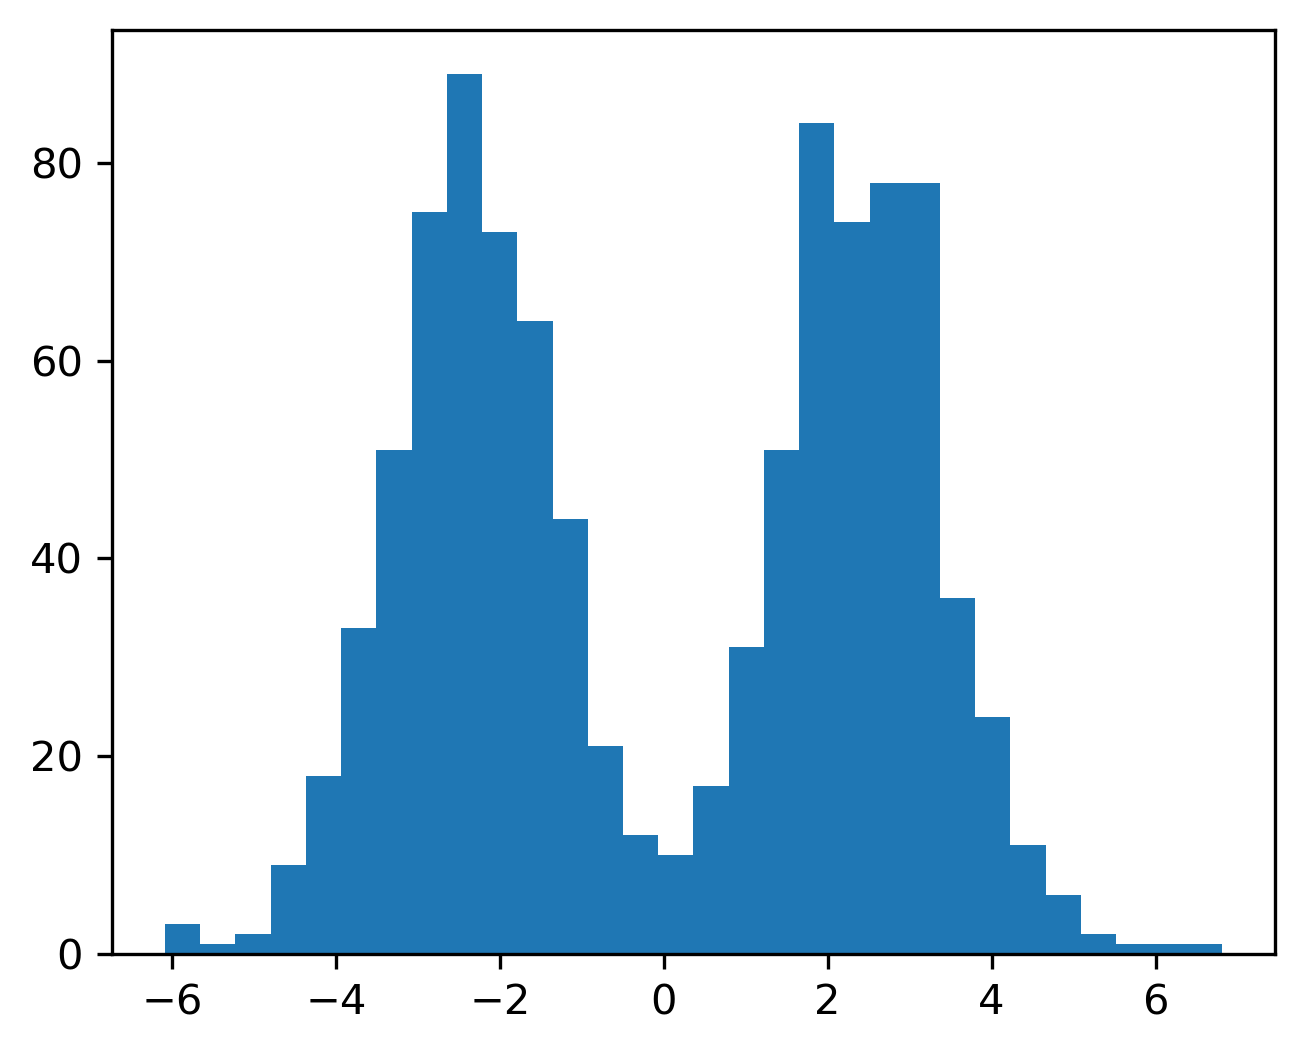
\includegraphics[width=0.48\linewidth]{images/2_cluster_hist_t_0.4.png}
                \caption{Распределение синтетического набора данных с параметром \(t = 0.4\).}
                \label{fig:synthetic:t:0.4}
            \end{figure}

            \begin{figure}[H]\centering
                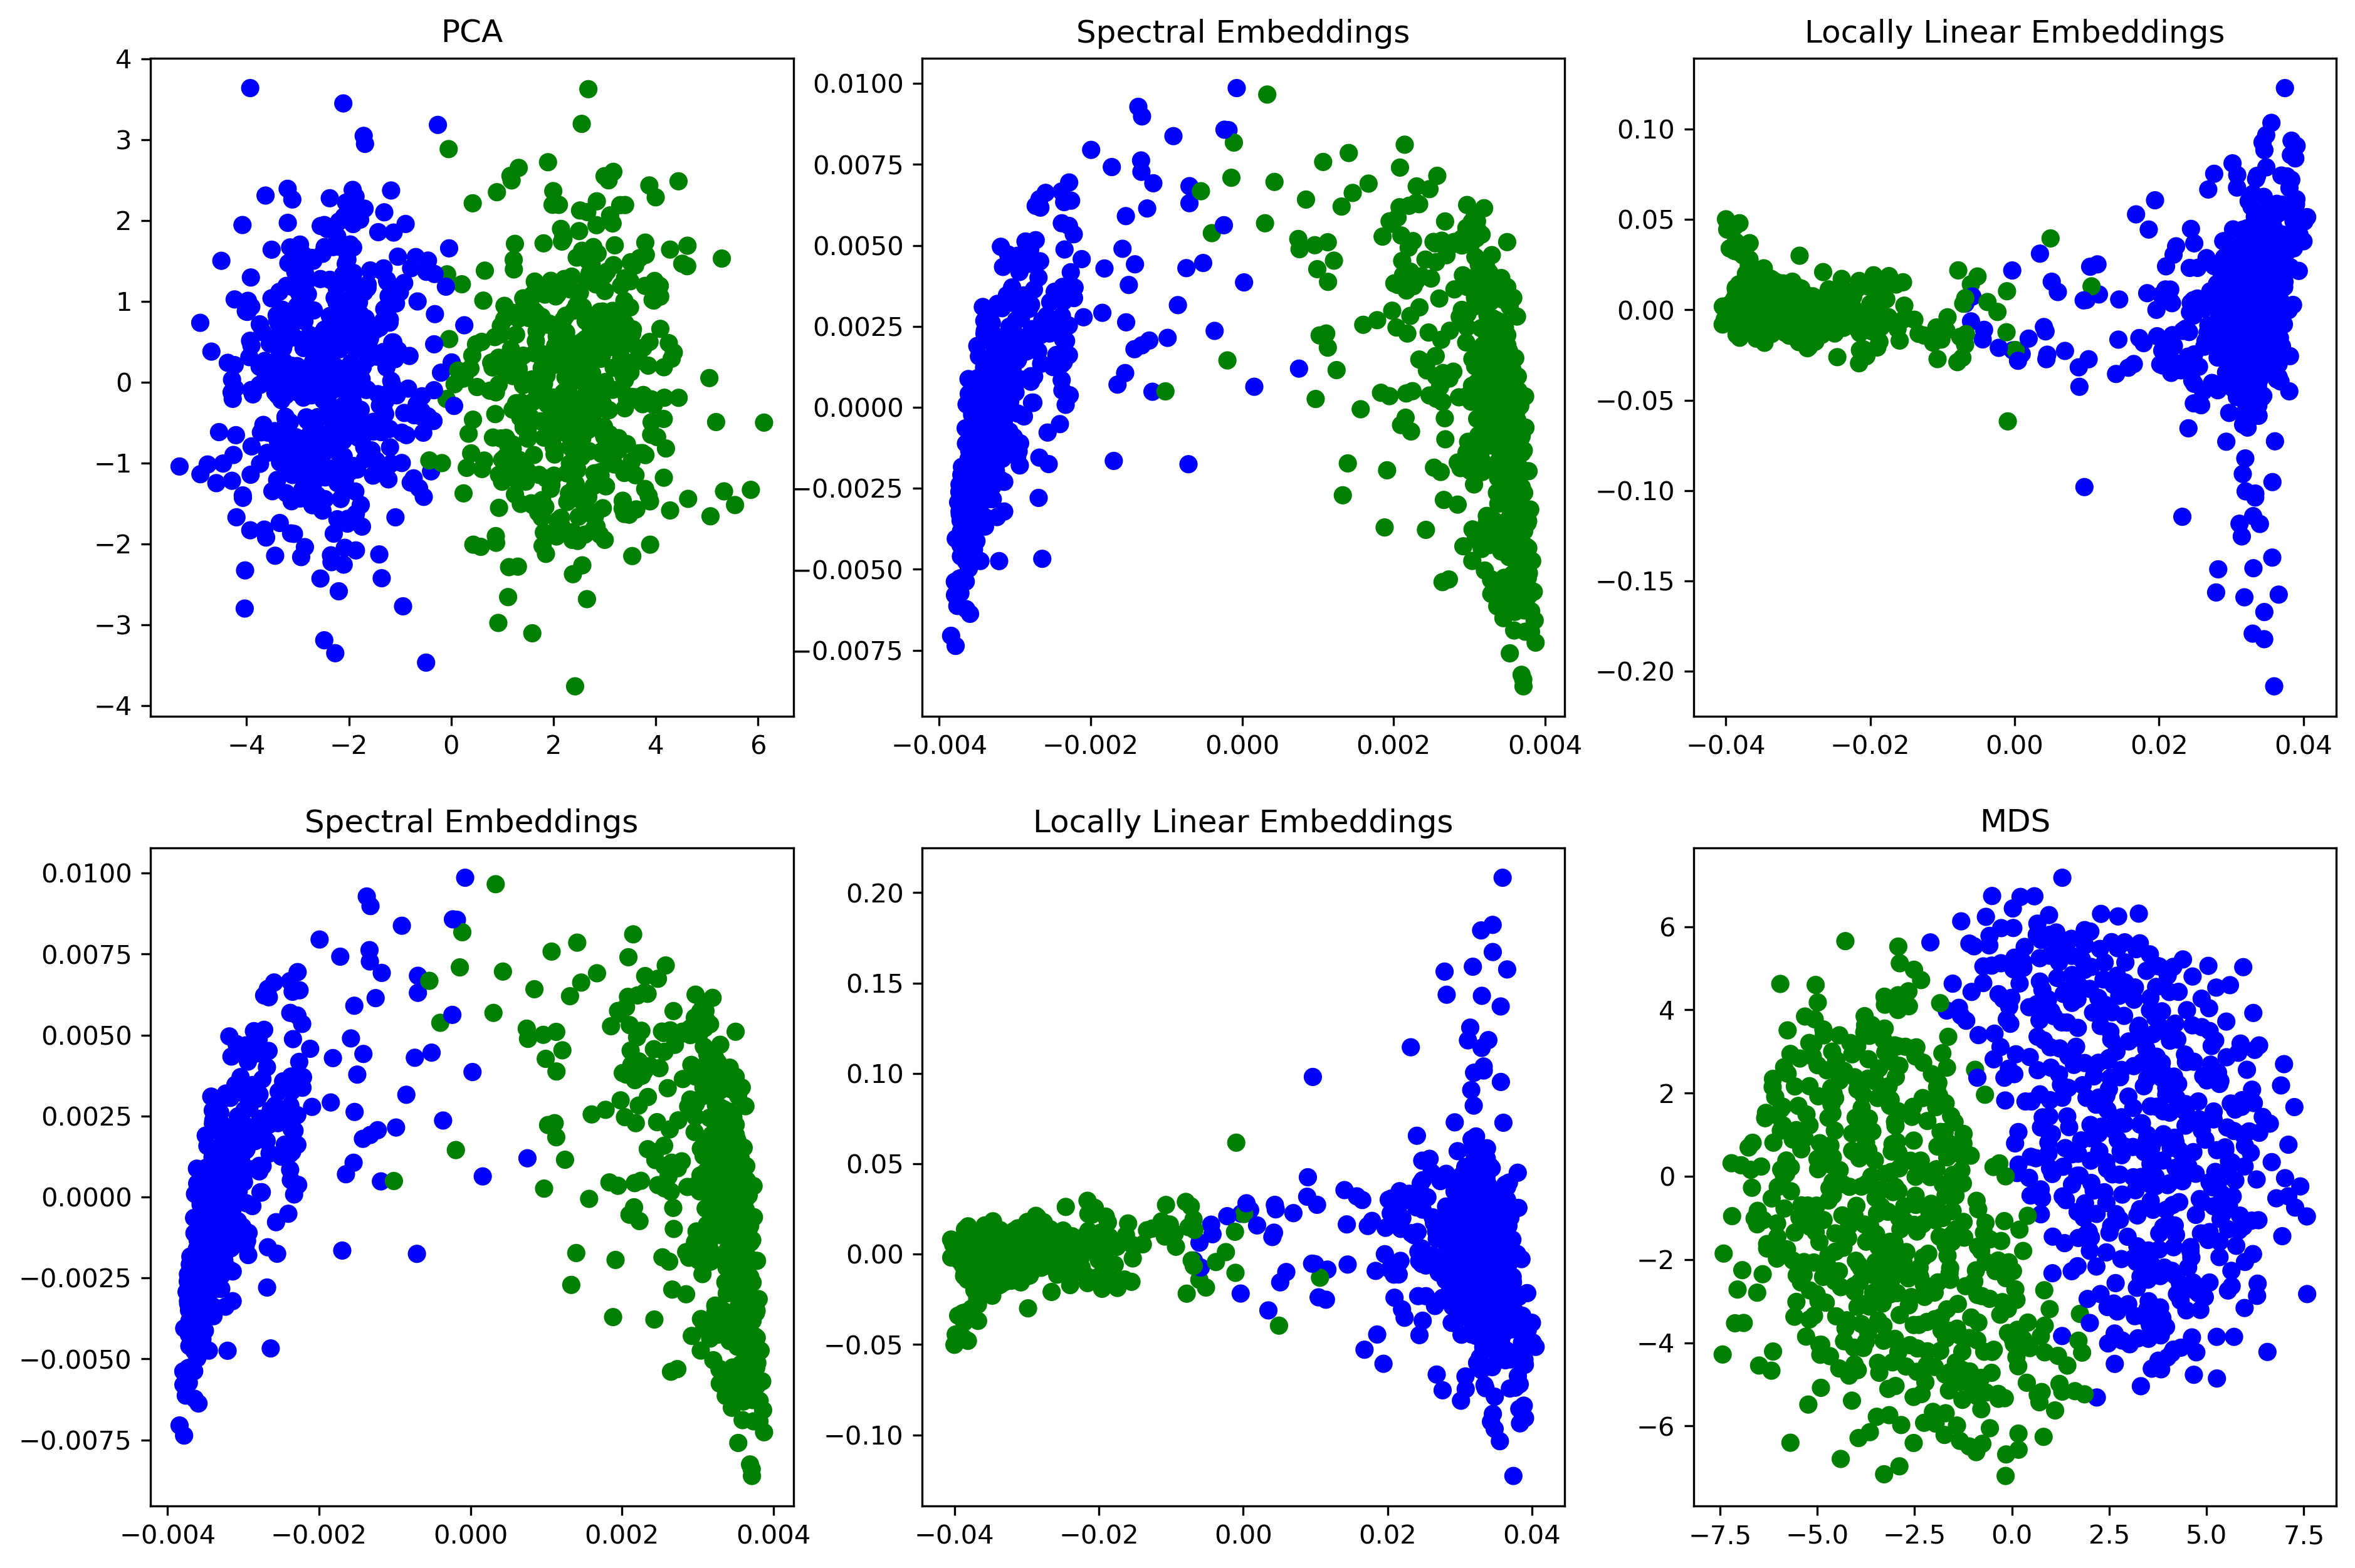
\includegraphics[width=0.99\linewidth]{images/decomposer/2_cluster_decomposer_analysis_t_0.4.png}
                \caption{Визуализация синтетических данных с параметром \(t = 0.4\) после снижения размерности с 20 до 2 с использованием PCA, Spectral Embeddings, Locally Linear Embeddings, MDS, ISOMAP, UMAP.}
                \label{fig:synthetic:t:0.4:example}
            \end{figure}

            Исходя из графиков, можно выделить явного лидера -- метод PCA, который стабильно показывает максимальные значения метрик (порядка 0.9 и выше) при любом количестве компонент. Это указывает на эффективное сохранение линейной структуры синтетических данных, особенно в случаях, когда кластеры умеренно разделены. MDS, а также ISOMAP и UMAP, дают сопоставимо высокие результаты, практически не зависящие от количества компонент, что говорит о слабой деградации качества даже при сильном снижении размерности данных. Locally Linear Embeddings и Spectral Embeddings, напротив, демонстрируют выраженную чувствительность к размерности. С уменьшением числа компонент качество кластеризации постепенно улучшается и достигает пика на размерности равной числу заложенных кластеров.

            \begin{figure}[H]\centering
                \subfigure[]{
                    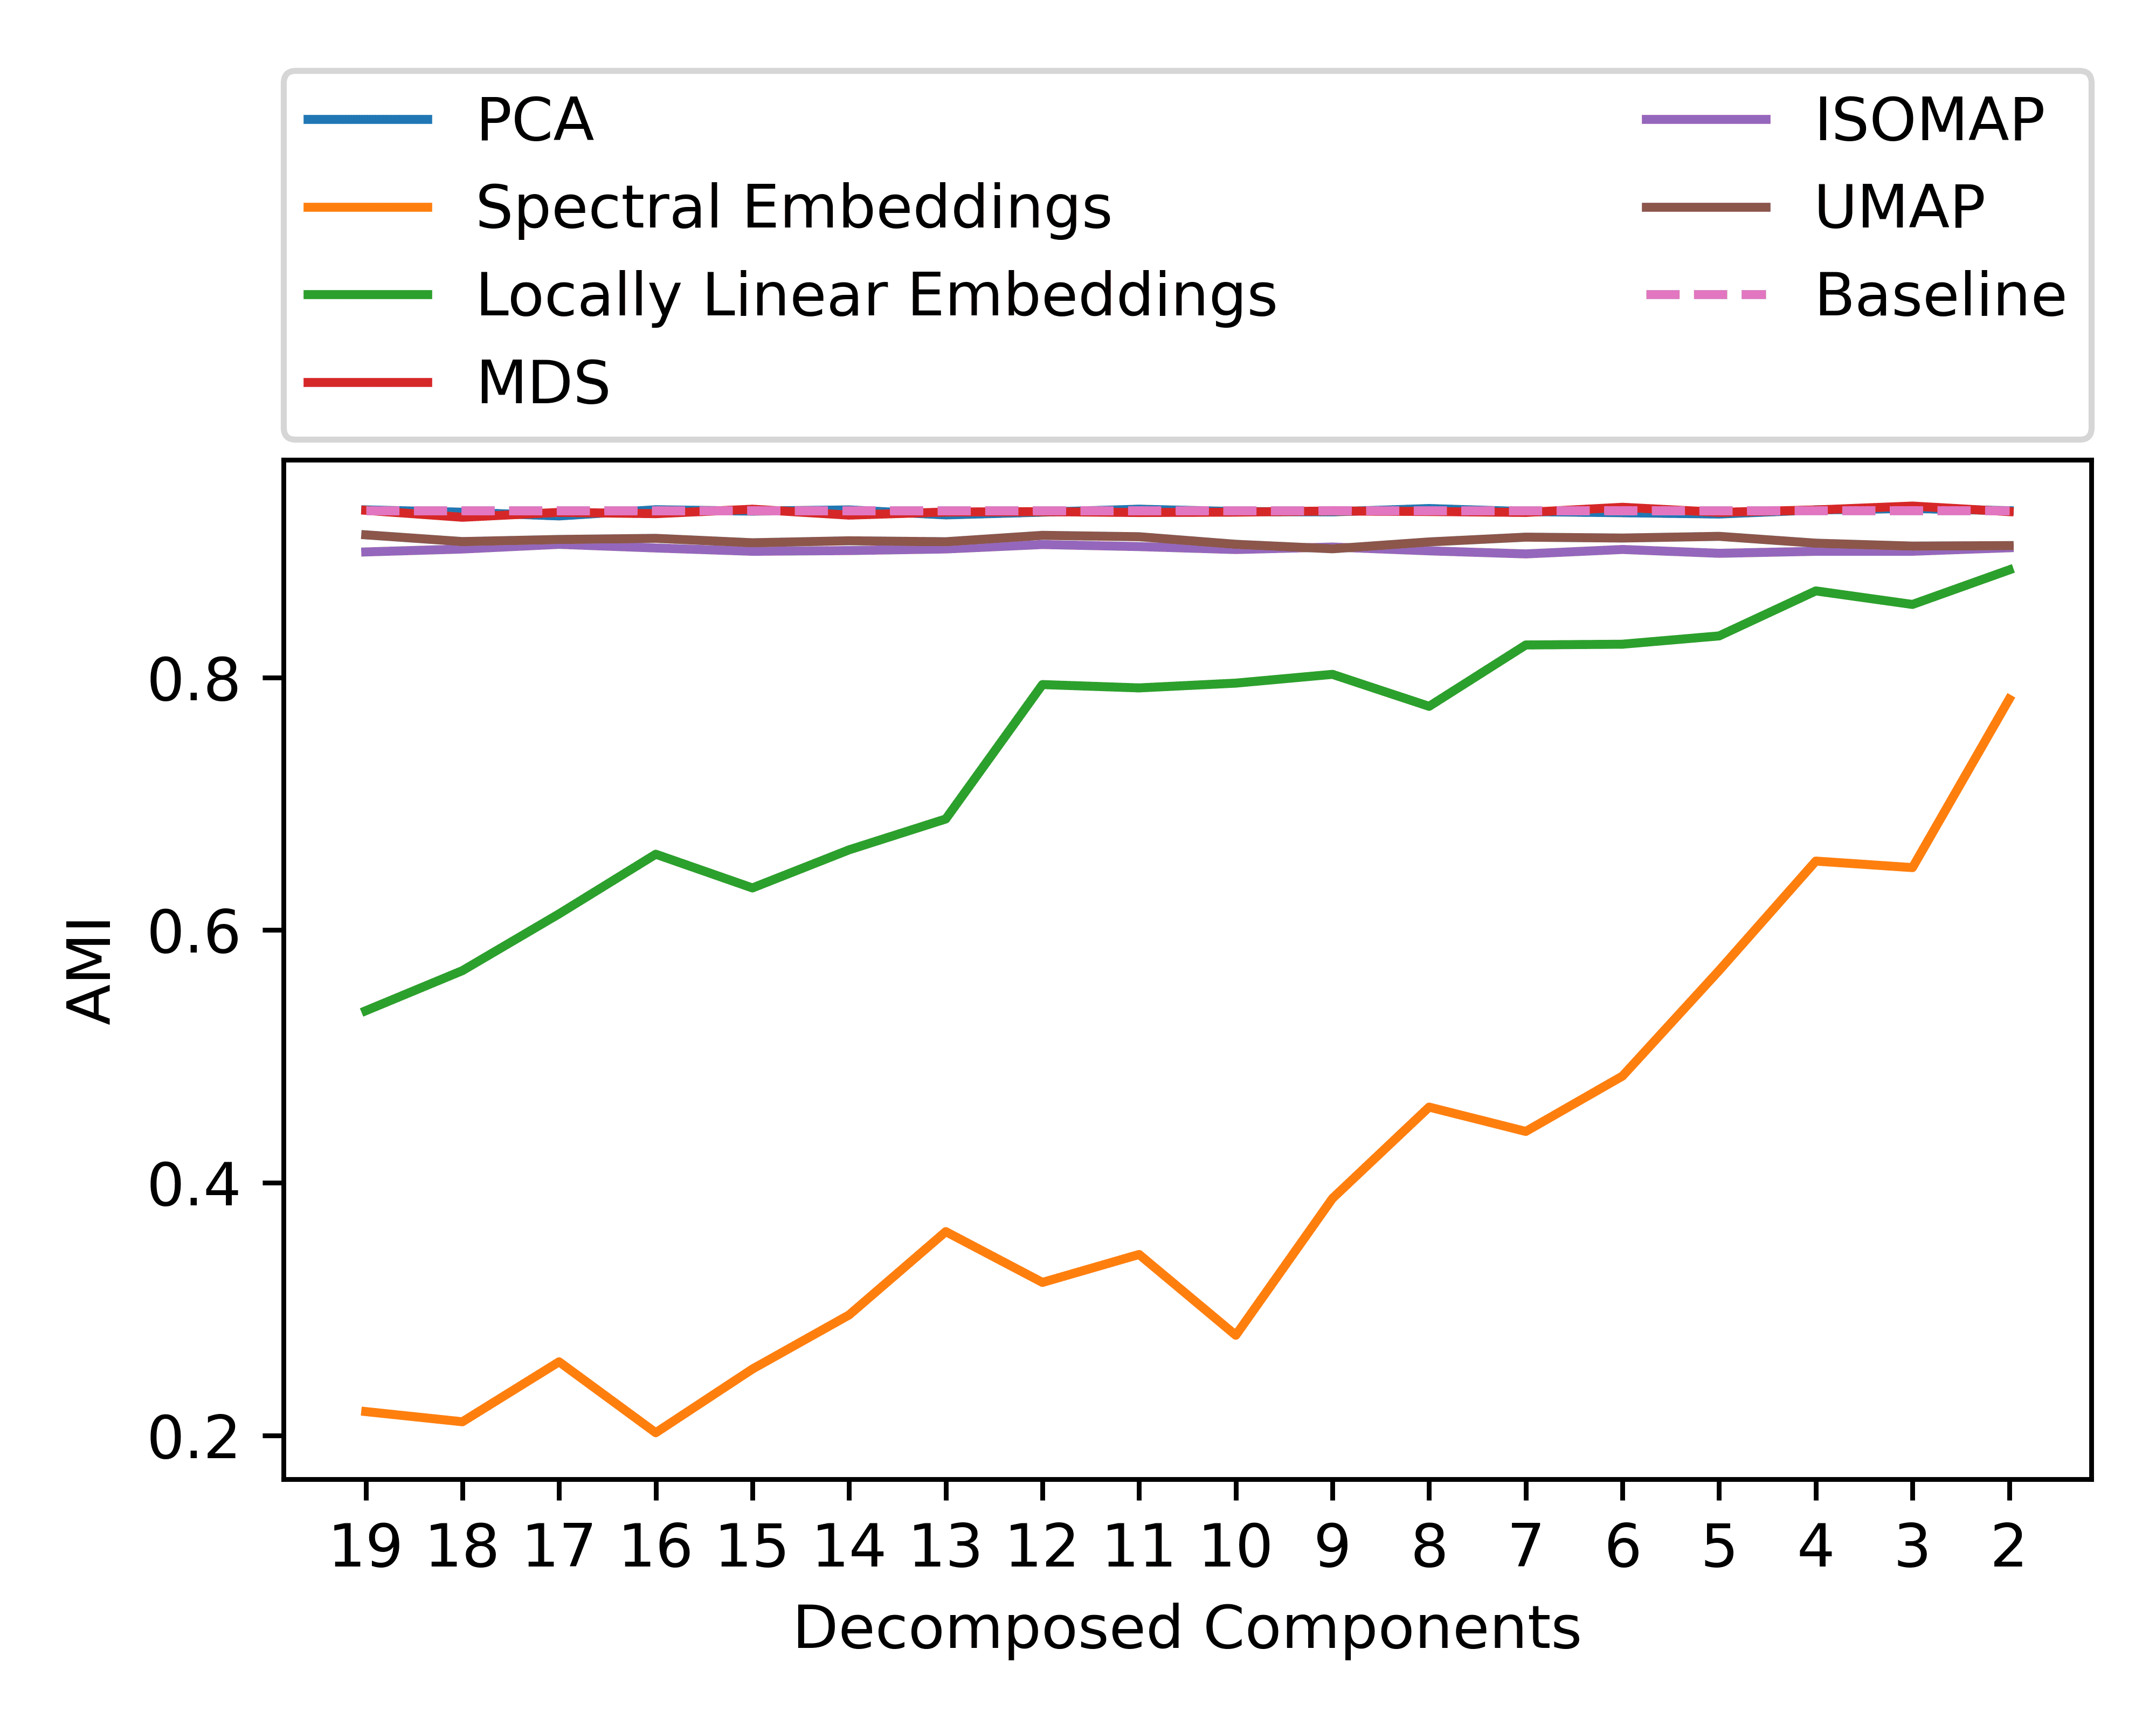
\includegraphics[width=0.48\linewidth]{images/charts/detailed_decomposition_metric_t_0.4_p_2_comparison_2_clusters_ami.png}
                    \label{subfig:synthetic:t_0.4:dim_influence:ami}
                }
                \subfigure[]{
                    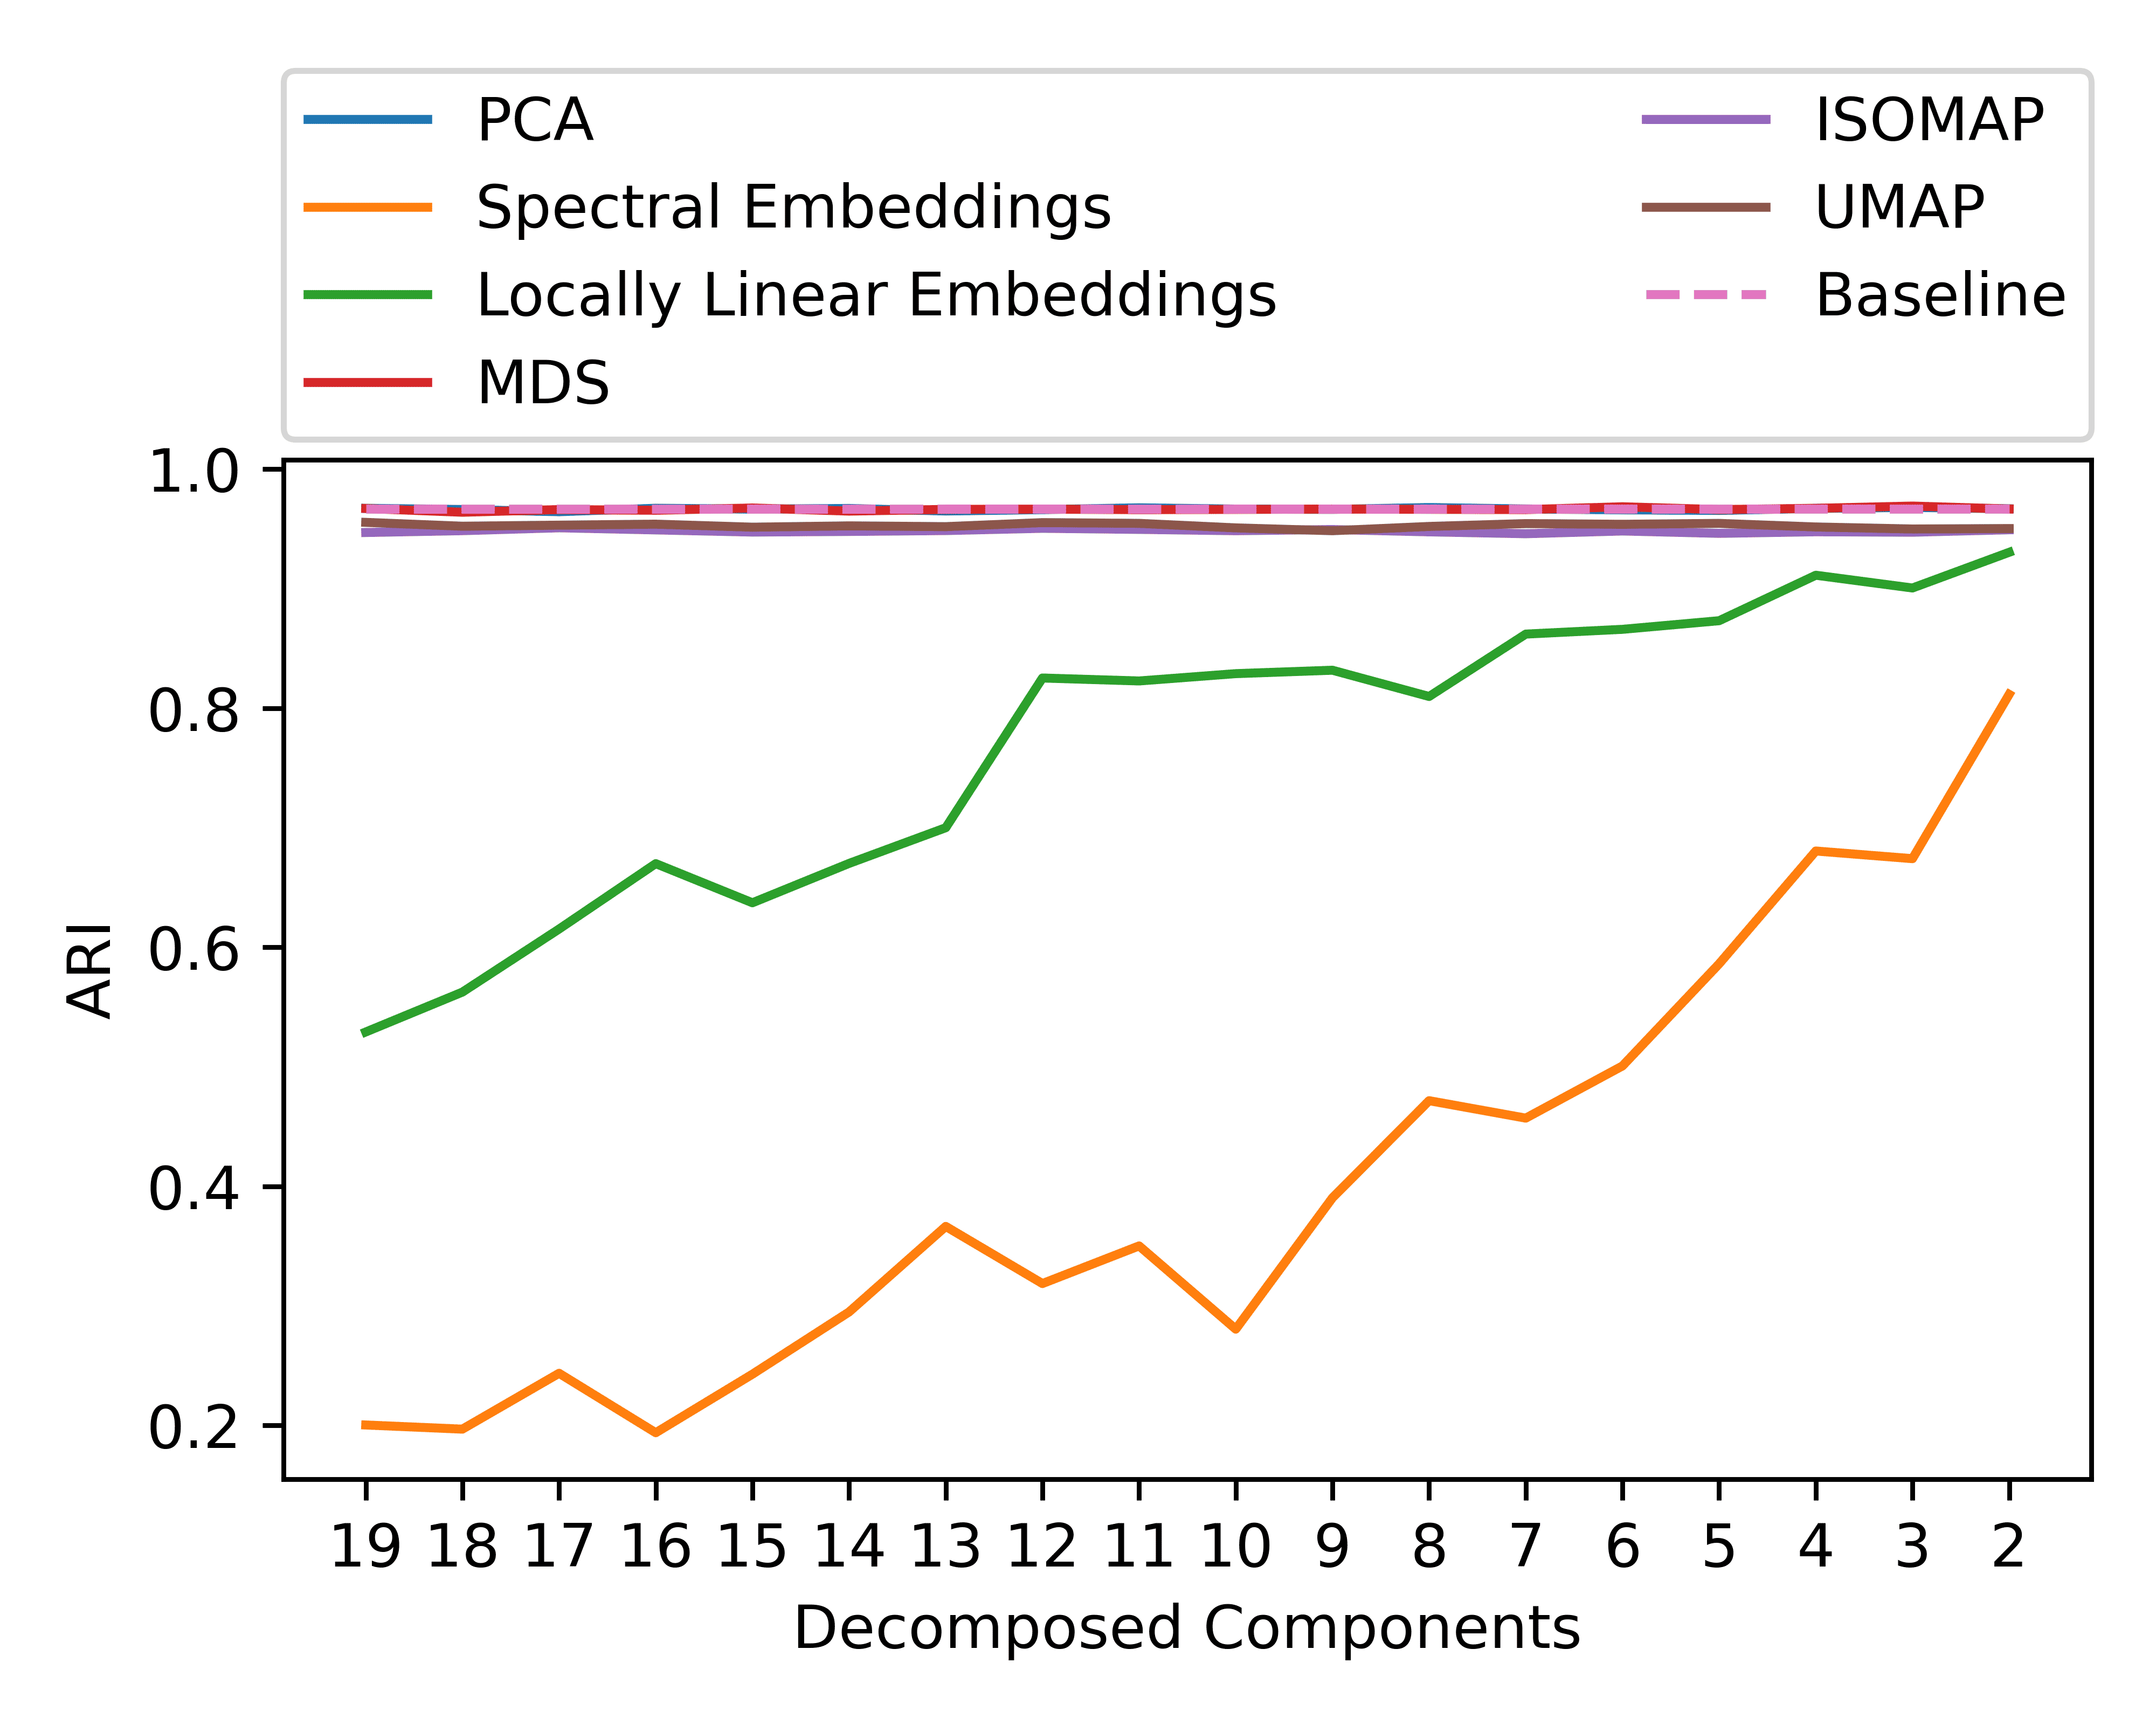
\includegraphics[width=0.48\linewidth]{images/charts/detailed_decomposition_metric_t_0.4_p_2_comparison_2_clusters_ari.png}
                    \label{subfig:synthetic:t_0.4:dim_influence:ari}
                }
                \subfigure[]{
                    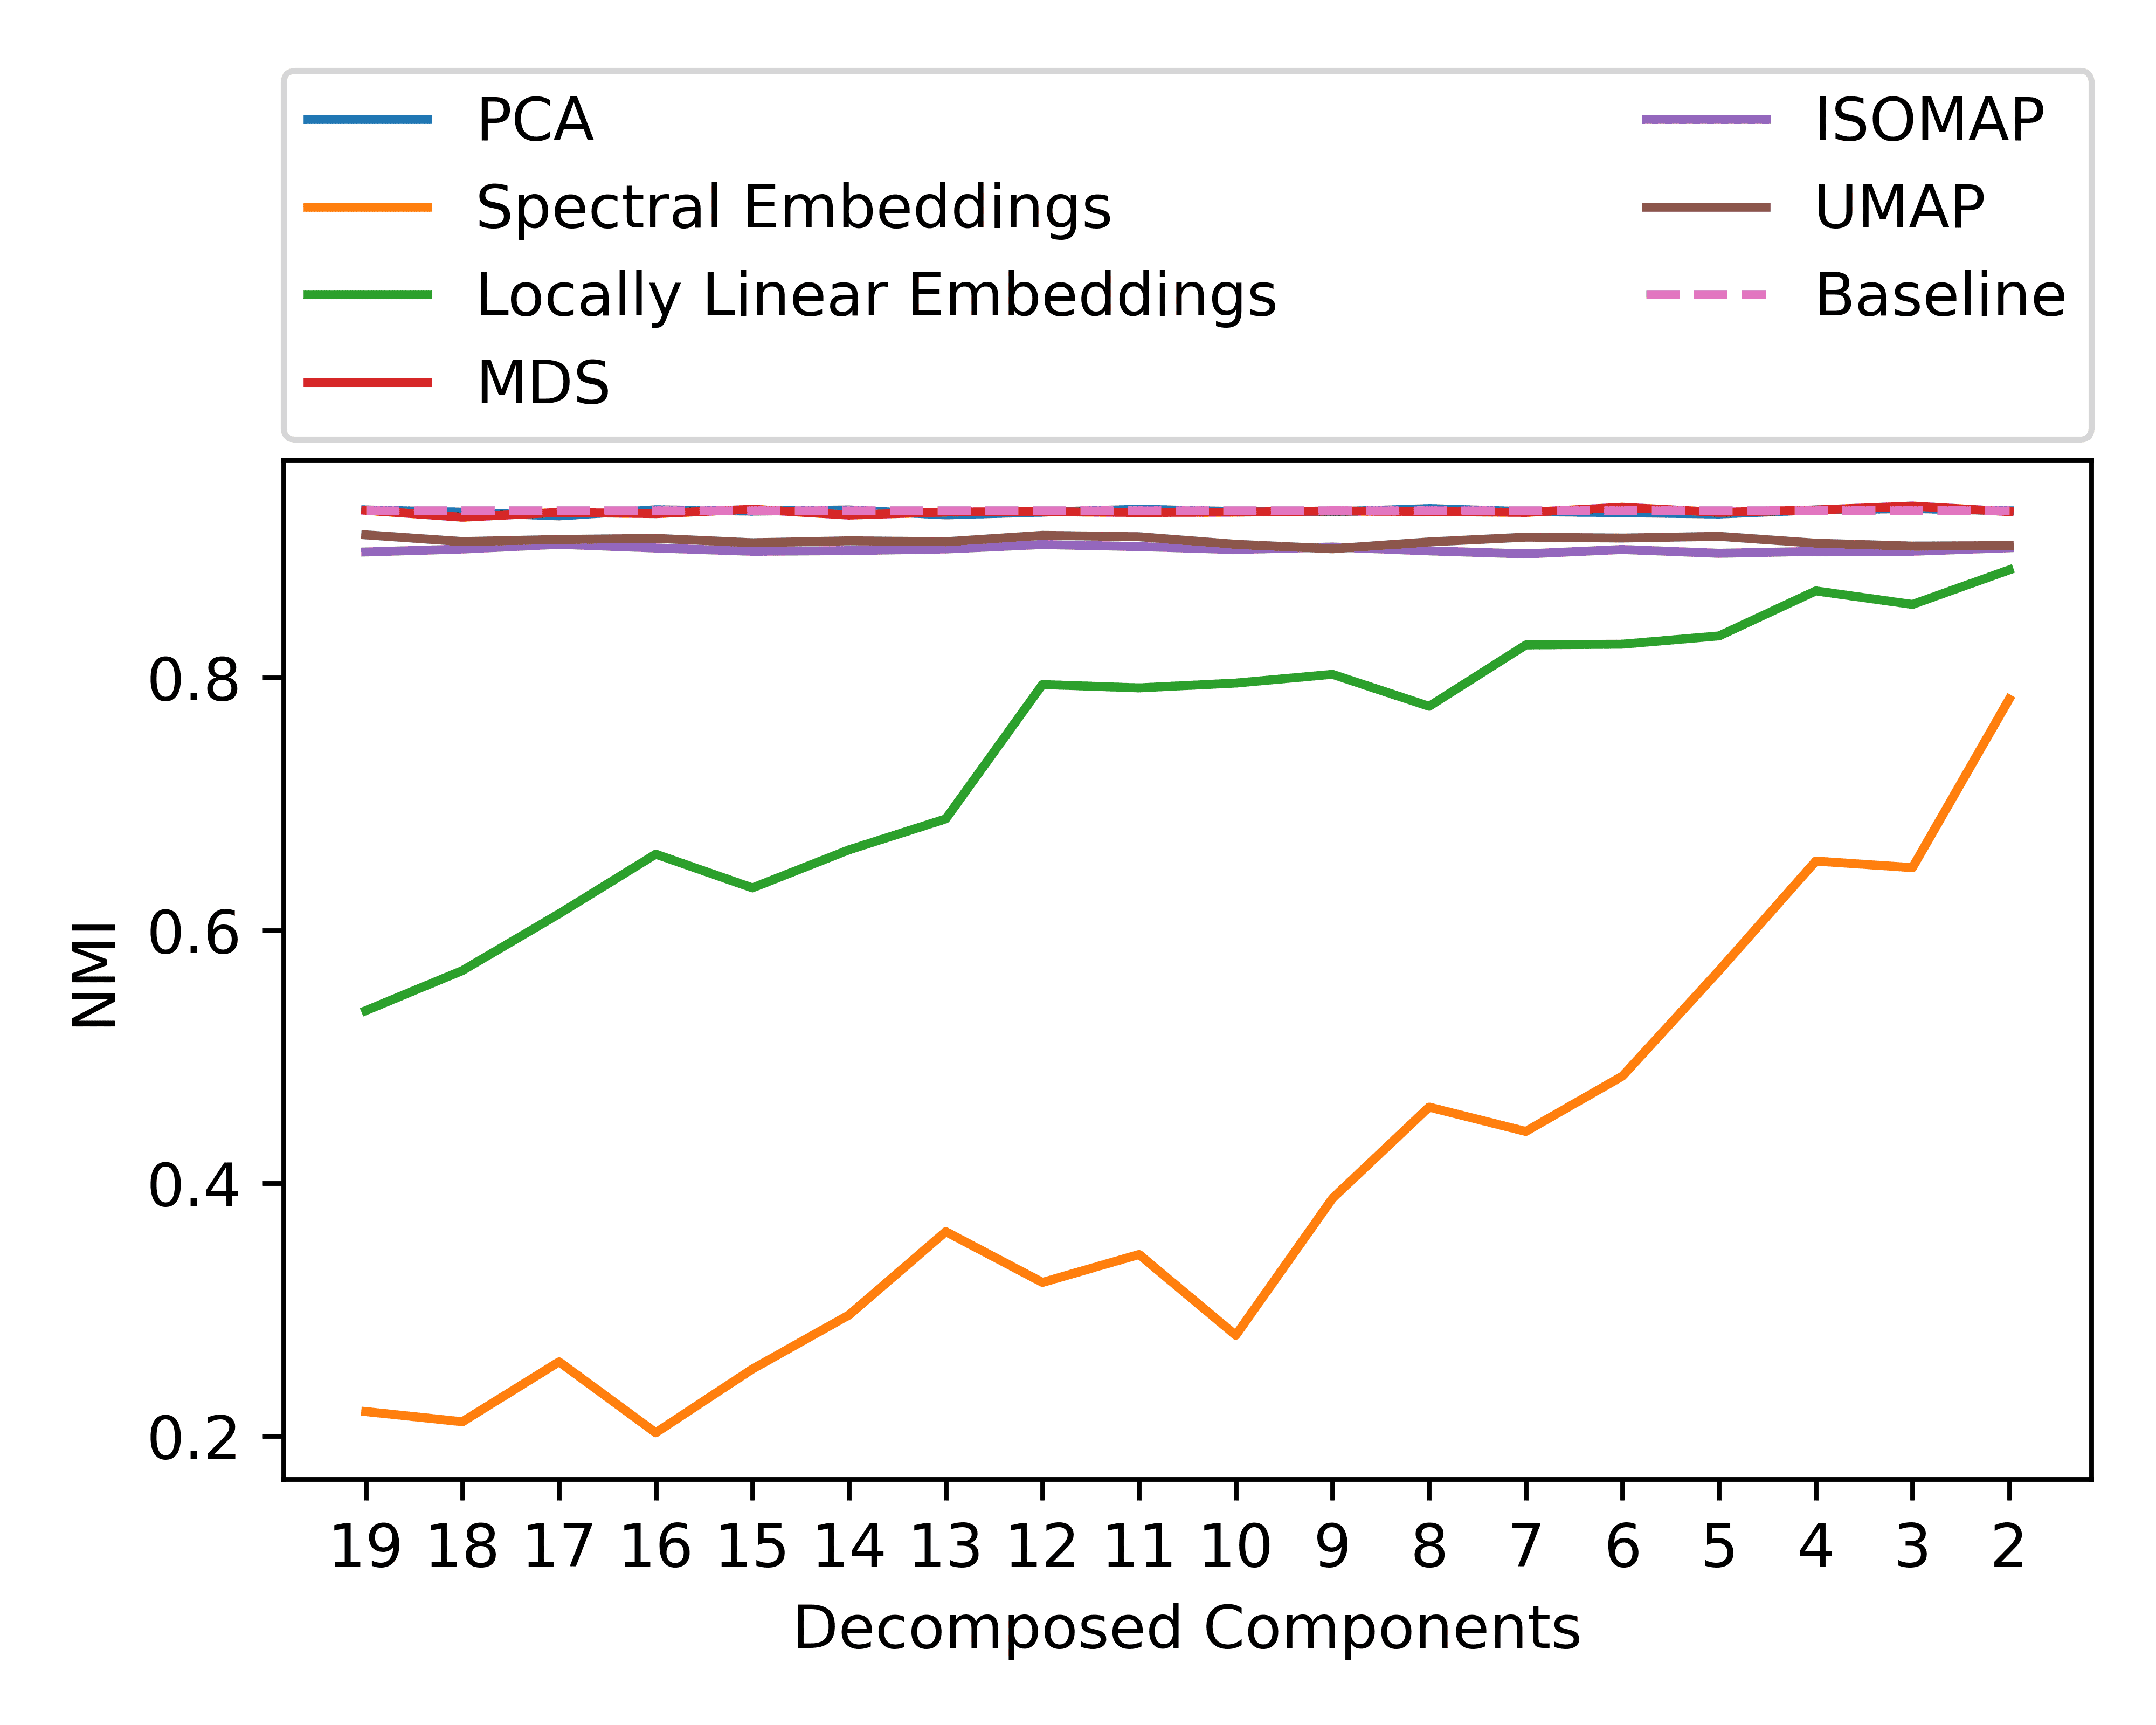
\includegraphics[width=0.48\linewidth]{images/charts/detailed_decomposition_metric_t_0.4_p_2_comparison_2_clusters_nmi.png}
                    \label{subfig:synthetic:t_0.4:dim_influence:nmi}
                }
                \subfigure[]{
                    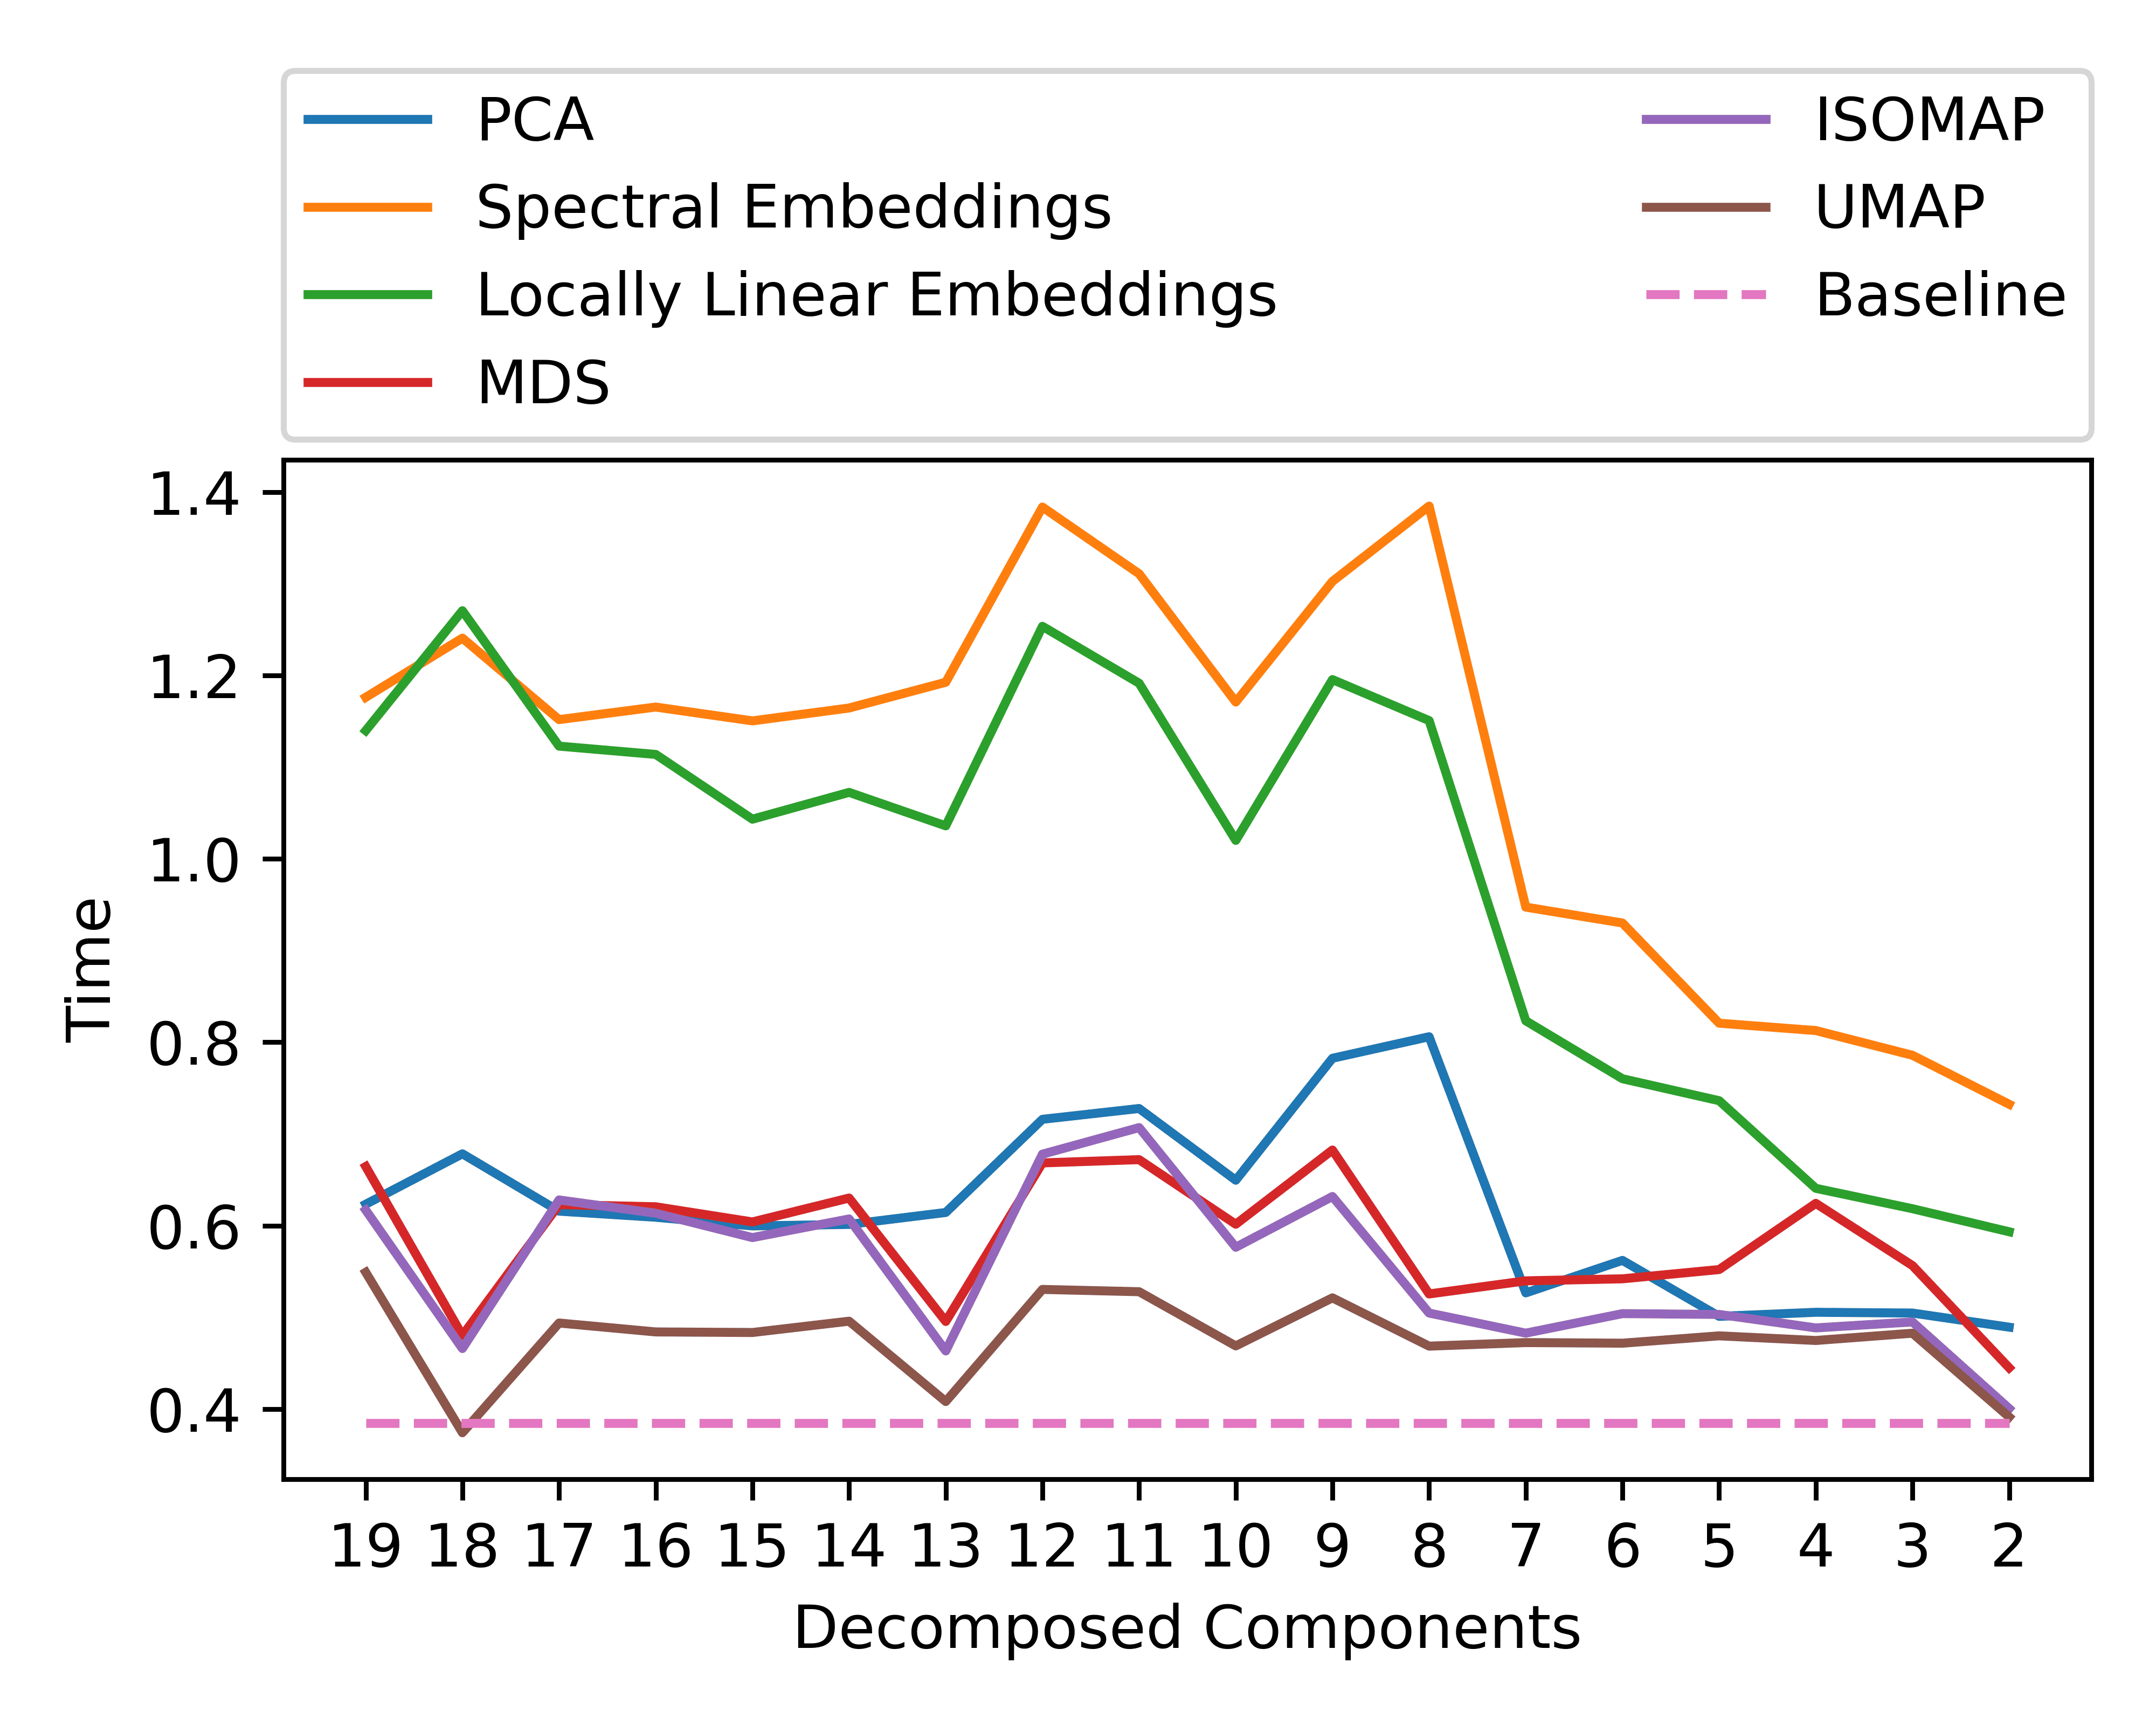
\includegraphics[width=0.48\linewidth]{images/charts/detailed_decomposition_metric_t_0.4_p_2_comparison_2_clusters_time.png}
                    \label{subfig:synthetic:t_0.4:dim_influence:time}
                }
                \caption{Анализ влияния размерности данных при различных методах снижения размерности на кластеризацию синтетического набора данных с параметром \(t = 0.4\). Линия Baseline -- результат работы алгоритма \kmeans{} без предварительного снижения размерности. Результаты для
                    \subref{subfig:synthetic:t_0.4:dim_influence:ami} AMI;
                    \subref{subfig:synthetic:t_0.4:dim_influence:ari} ARI;
                    \subref{subfig:synthetic:t_0.4:dim_influence:nmi} NMI, а также на время работы алгоритма \subref{subfig:synthetic:t_influence:time}.
                }
                \label{fig:synthetic:t_0.4:dim_influence}
            \end{figure}

            На рисунке \ref{fig:synthetic:t_0.8:dim_influence} представлен анализ влияния количества компонент, оставляемых после снижения размерности, на качество кластеризации при фиксированном значении параметра \(t = 0.8\), соответствующем сильному перекрытию кластеров (Рисунок \ref{fig:synthetic:t:0.8}). На этом уровне разделимость между группами минимальна, что делает задачу особенно чувствительной к качеству понижения размерности. Также, следует, что методы PCA демонстрирует наилучшую устойчивость и качество кластеризации вне зависимости от числа компонент. В противоположность, методы Locally Linear Embeddings и Spectral Embeddings показывают низкие и слабо возрастающие значения всех метрик при уменьшении количества компонент, что говорит о неэффективном представлении кластерной структуры в условиях высокой плотности и перекрытия. Рисунок \ref{fig:synthetic:t:0.8:example} отображает распределение точек в пространстве меньшей размерности после применения методов снижения размерности PCA, Spectral Embeddings, Locally Linear Embeddings, MDS, ISOMAP, UMAP.

            \begin{figure}[H]\centering
                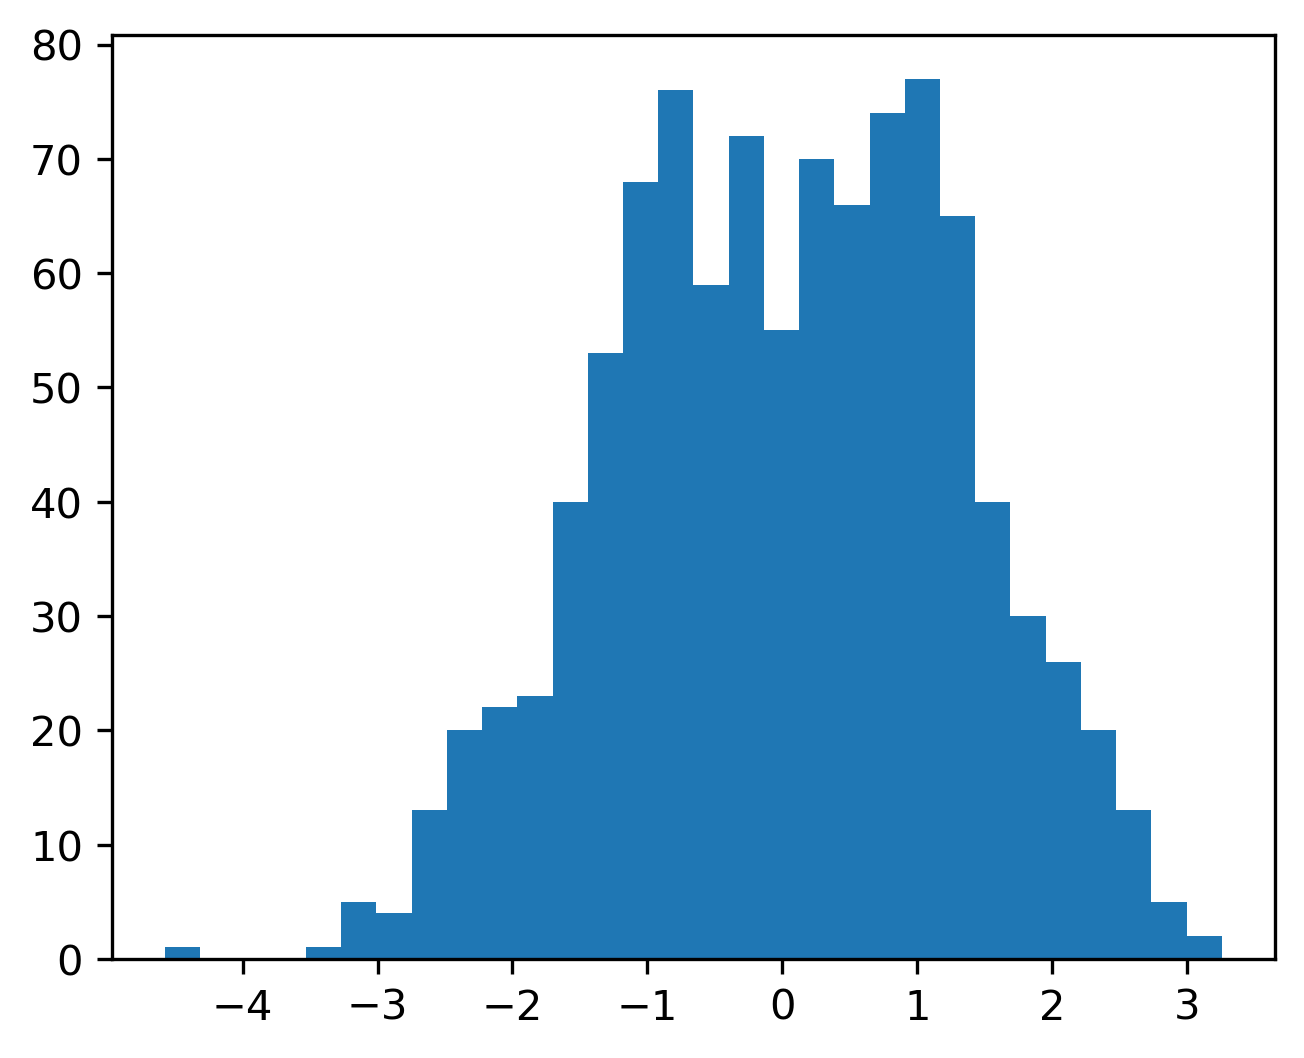
\includegraphics[width=0.48\linewidth]{images/2_cluster_hist_t_0.8.png}
                \caption{Распределение синтетического набора данных с параметром \(t = 0.8\).}
                \label{fig:synthetic:t:0.8}
            \end{figure}

            \begin{figure}[H]\centering
                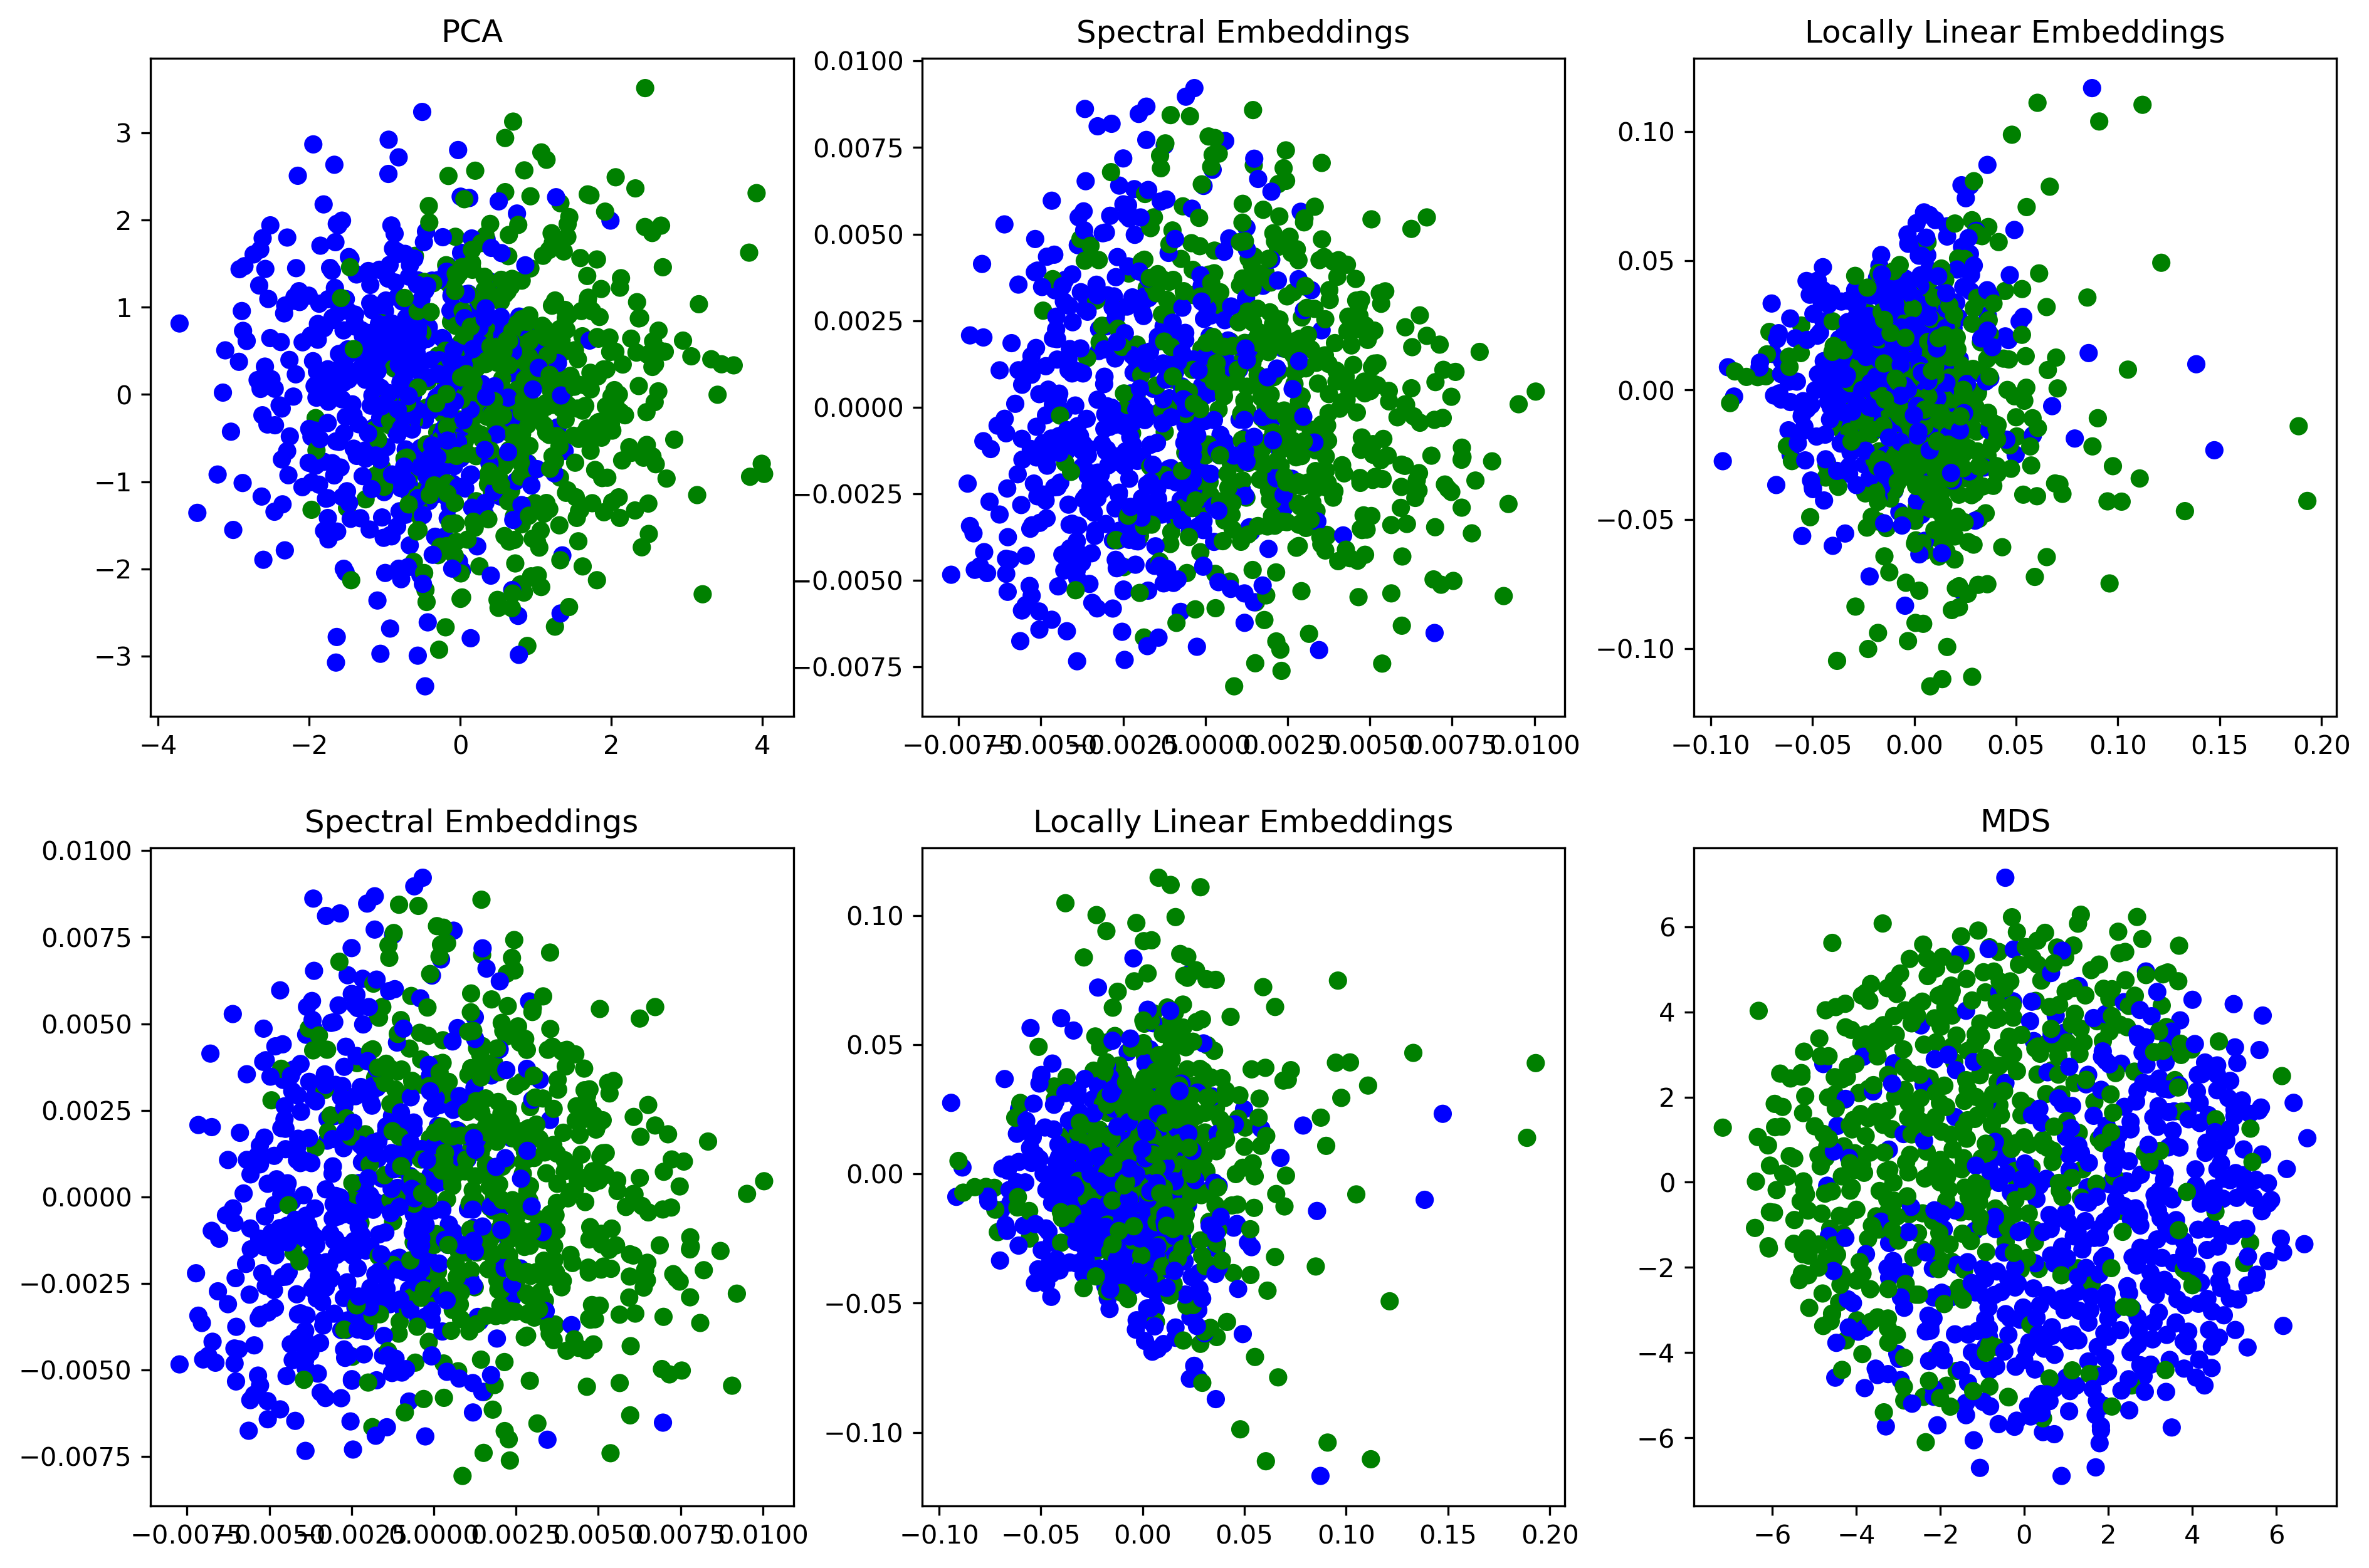
\includegraphics[width=0.99\linewidth]{images/decomposer/2_cluster_decomposer_analysis_t_0.8.png}
                \caption{Визуализация синтетических данных с параметром \(t = 0.8\) после снижения размерности с 20 до 2 с использованием PCA, Spectral Embeddings, Locally Linear Embeddings, MDS, ISOMAP, UMAP.}
                \label{fig:synthetic:t:0.8:example}
            \end{figure}

            Таким образом, при высоком уровне наложения кластеров (большое t) и варьируемом числе компонент, наиболее стабильные и надежные результаты обеспечивают методы PCA и MDS. Остальные методы, особенно LLE и Spectral, оказываются крайне чувствительными к размерности и не рекомендованы к применению в таких условиях.

            \begin{figure}[H]\centering
                \subfigure[]{
                    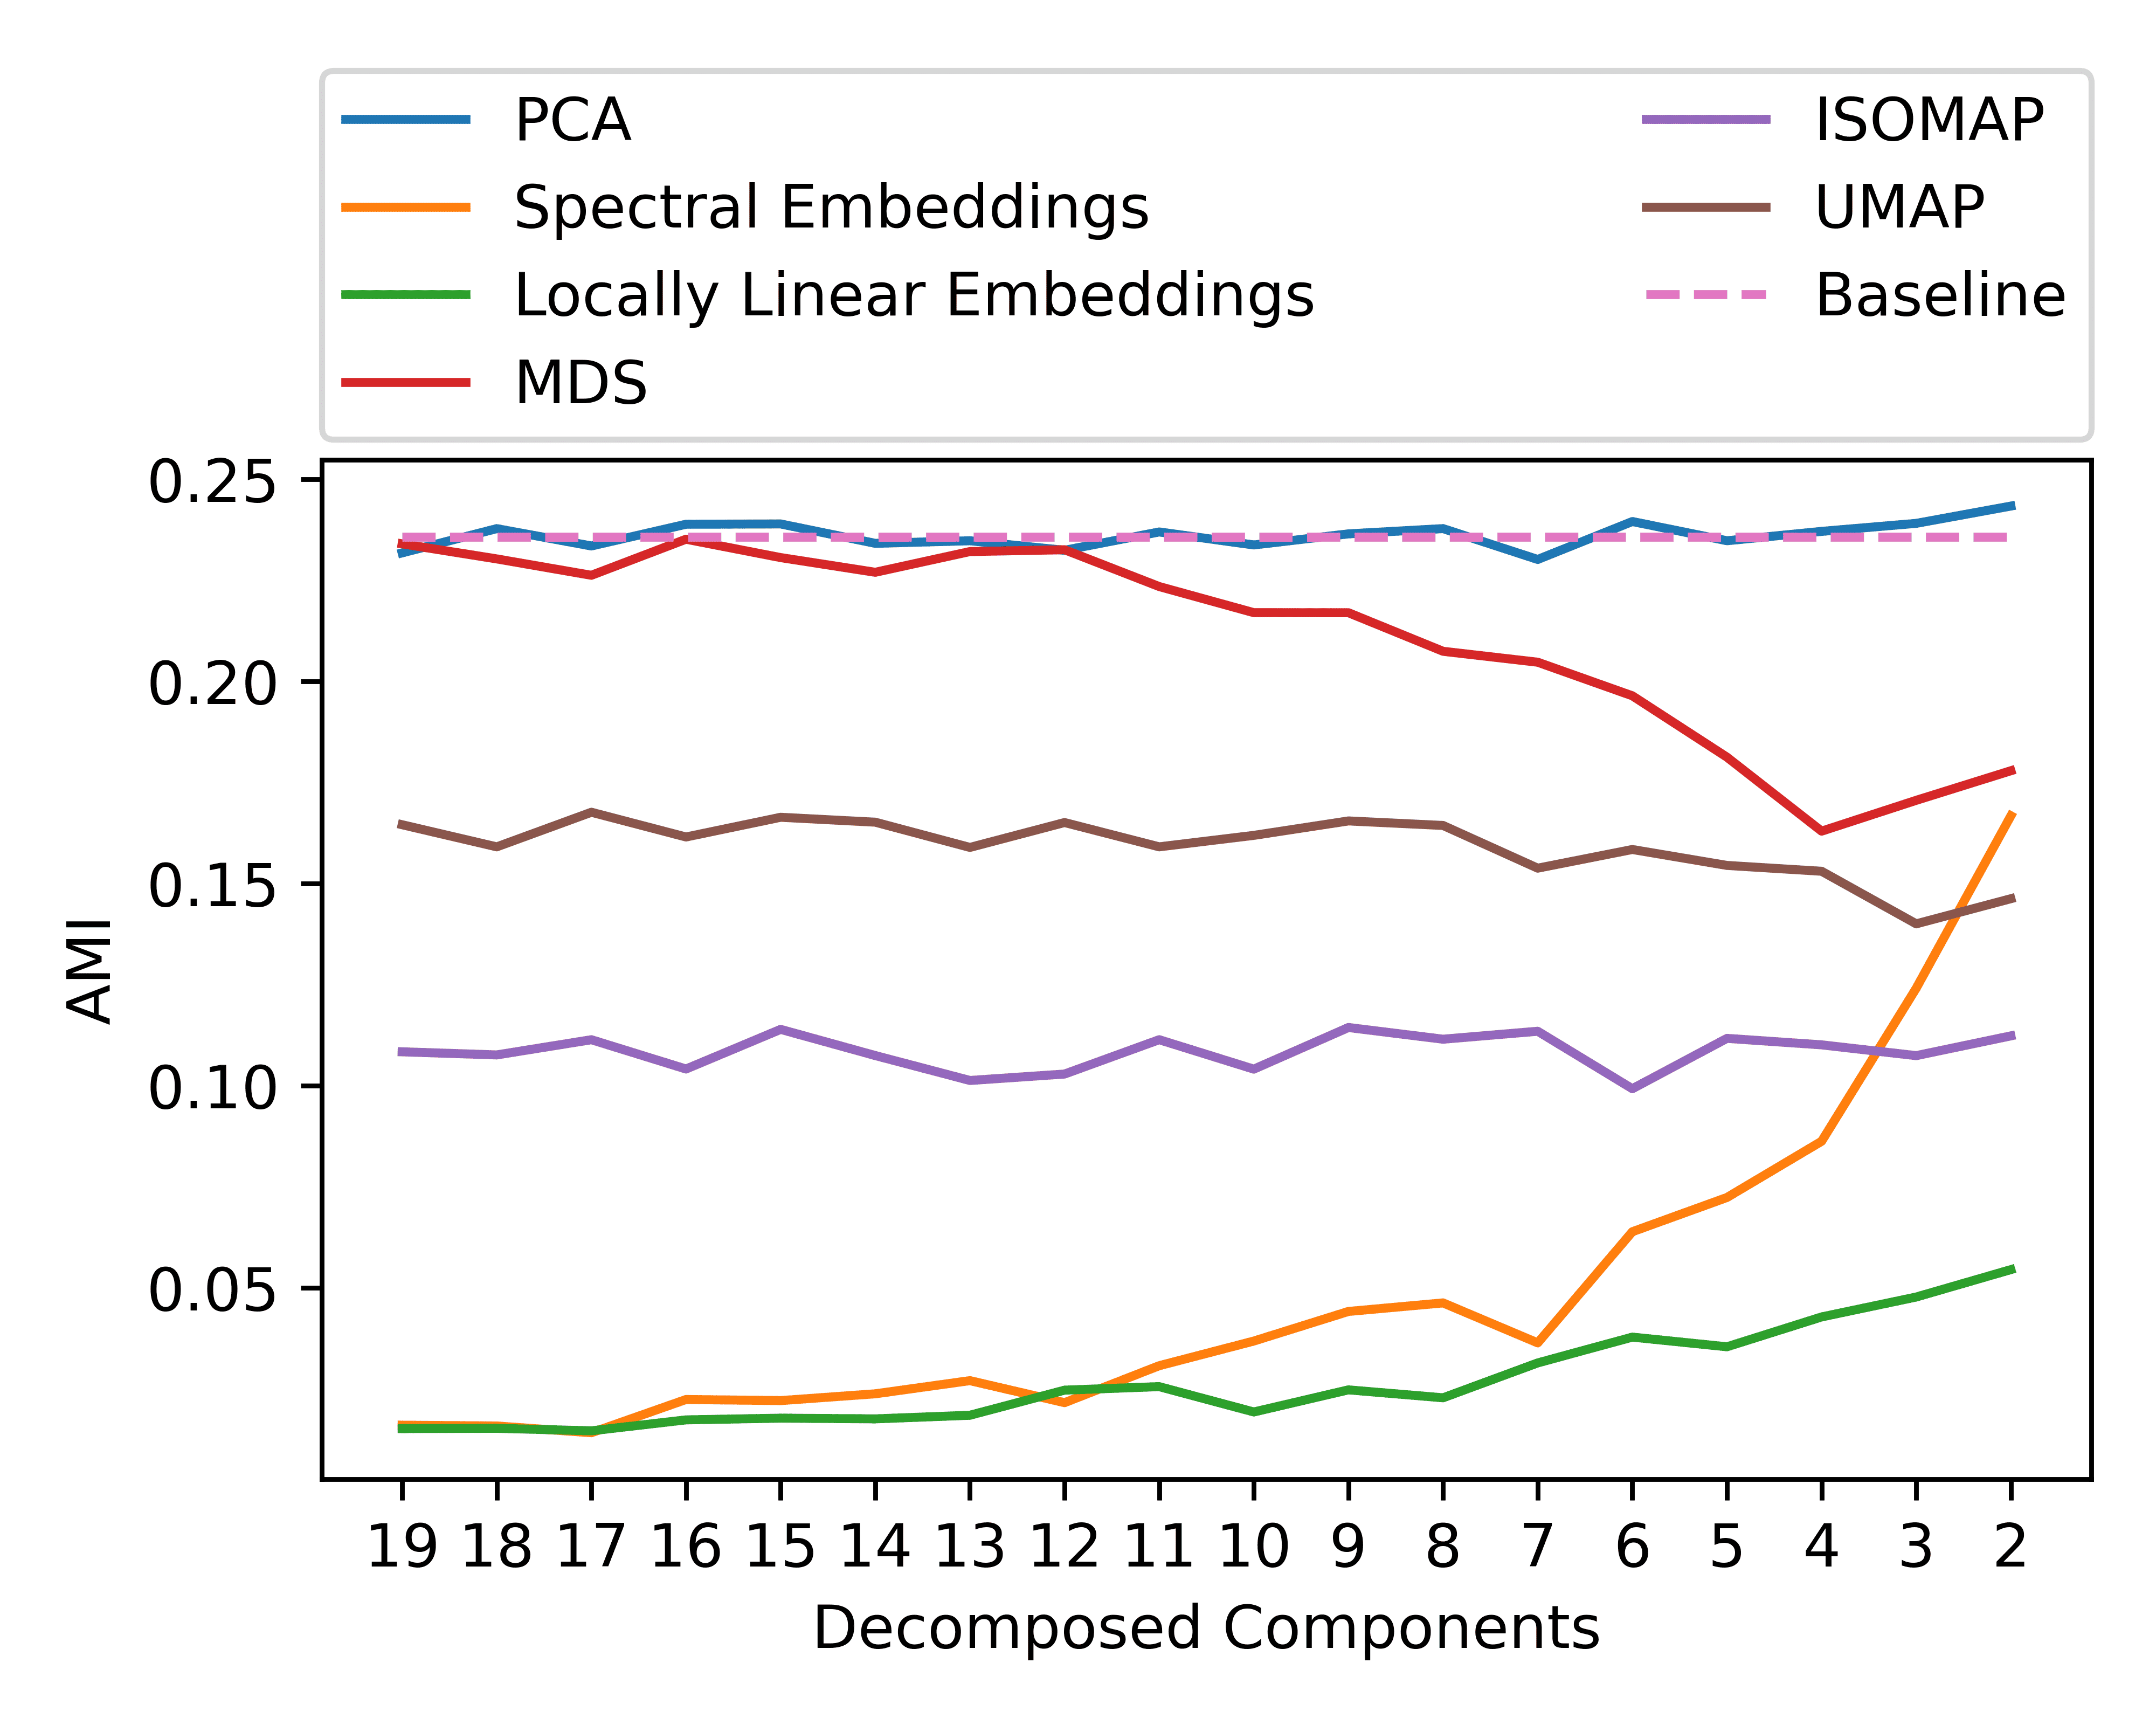
\includegraphics[width=0.48\linewidth]{images/charts/detailed_decomposition_metric_t_0.8_p_2_comparison_2_clusters_ami.png}
                    \label{subfig:synthetic:t_0.8:dim_influence:ami}
                }
                \subfigure[]{
                    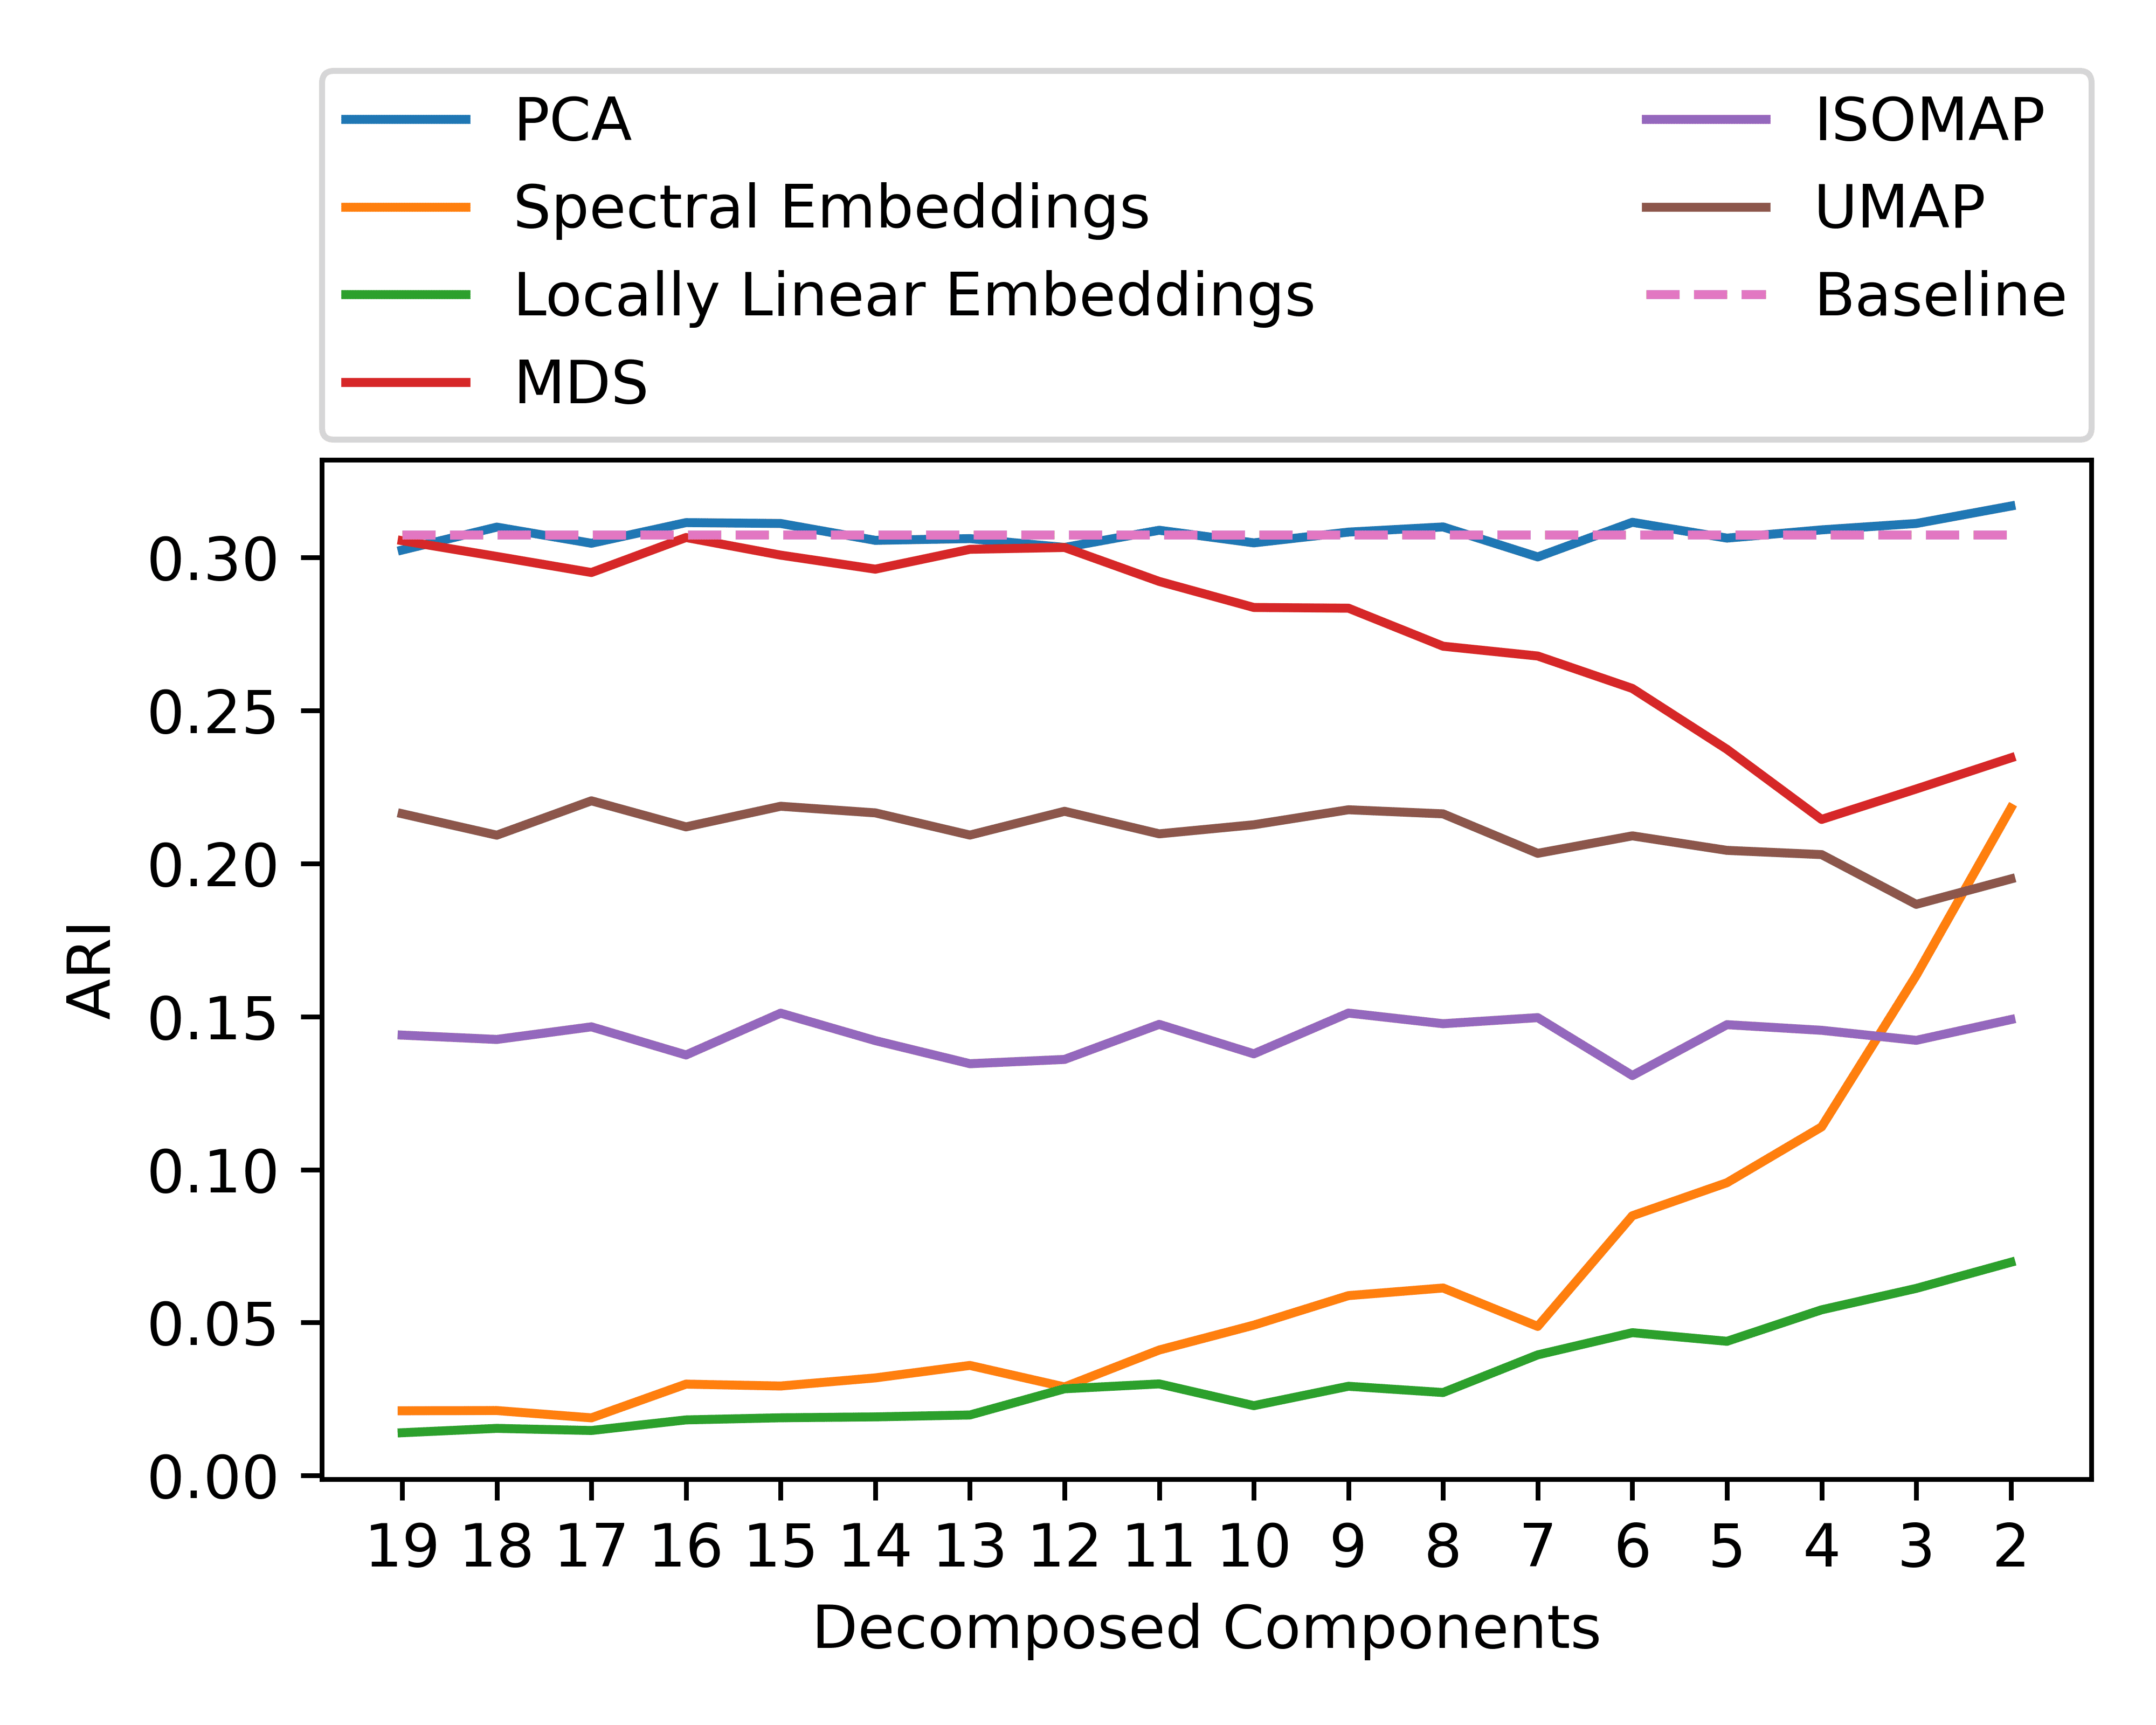
\includegraphics[width=0.48\linewidth]{images/charts/detailed_decomposition_metric_t_0.8_p_2_comparison_2_clusters_ari.png}
                    \label{subfig:synthetic:t_0.8:dim_influence:ari}
                }
                \subfigure[]{
                    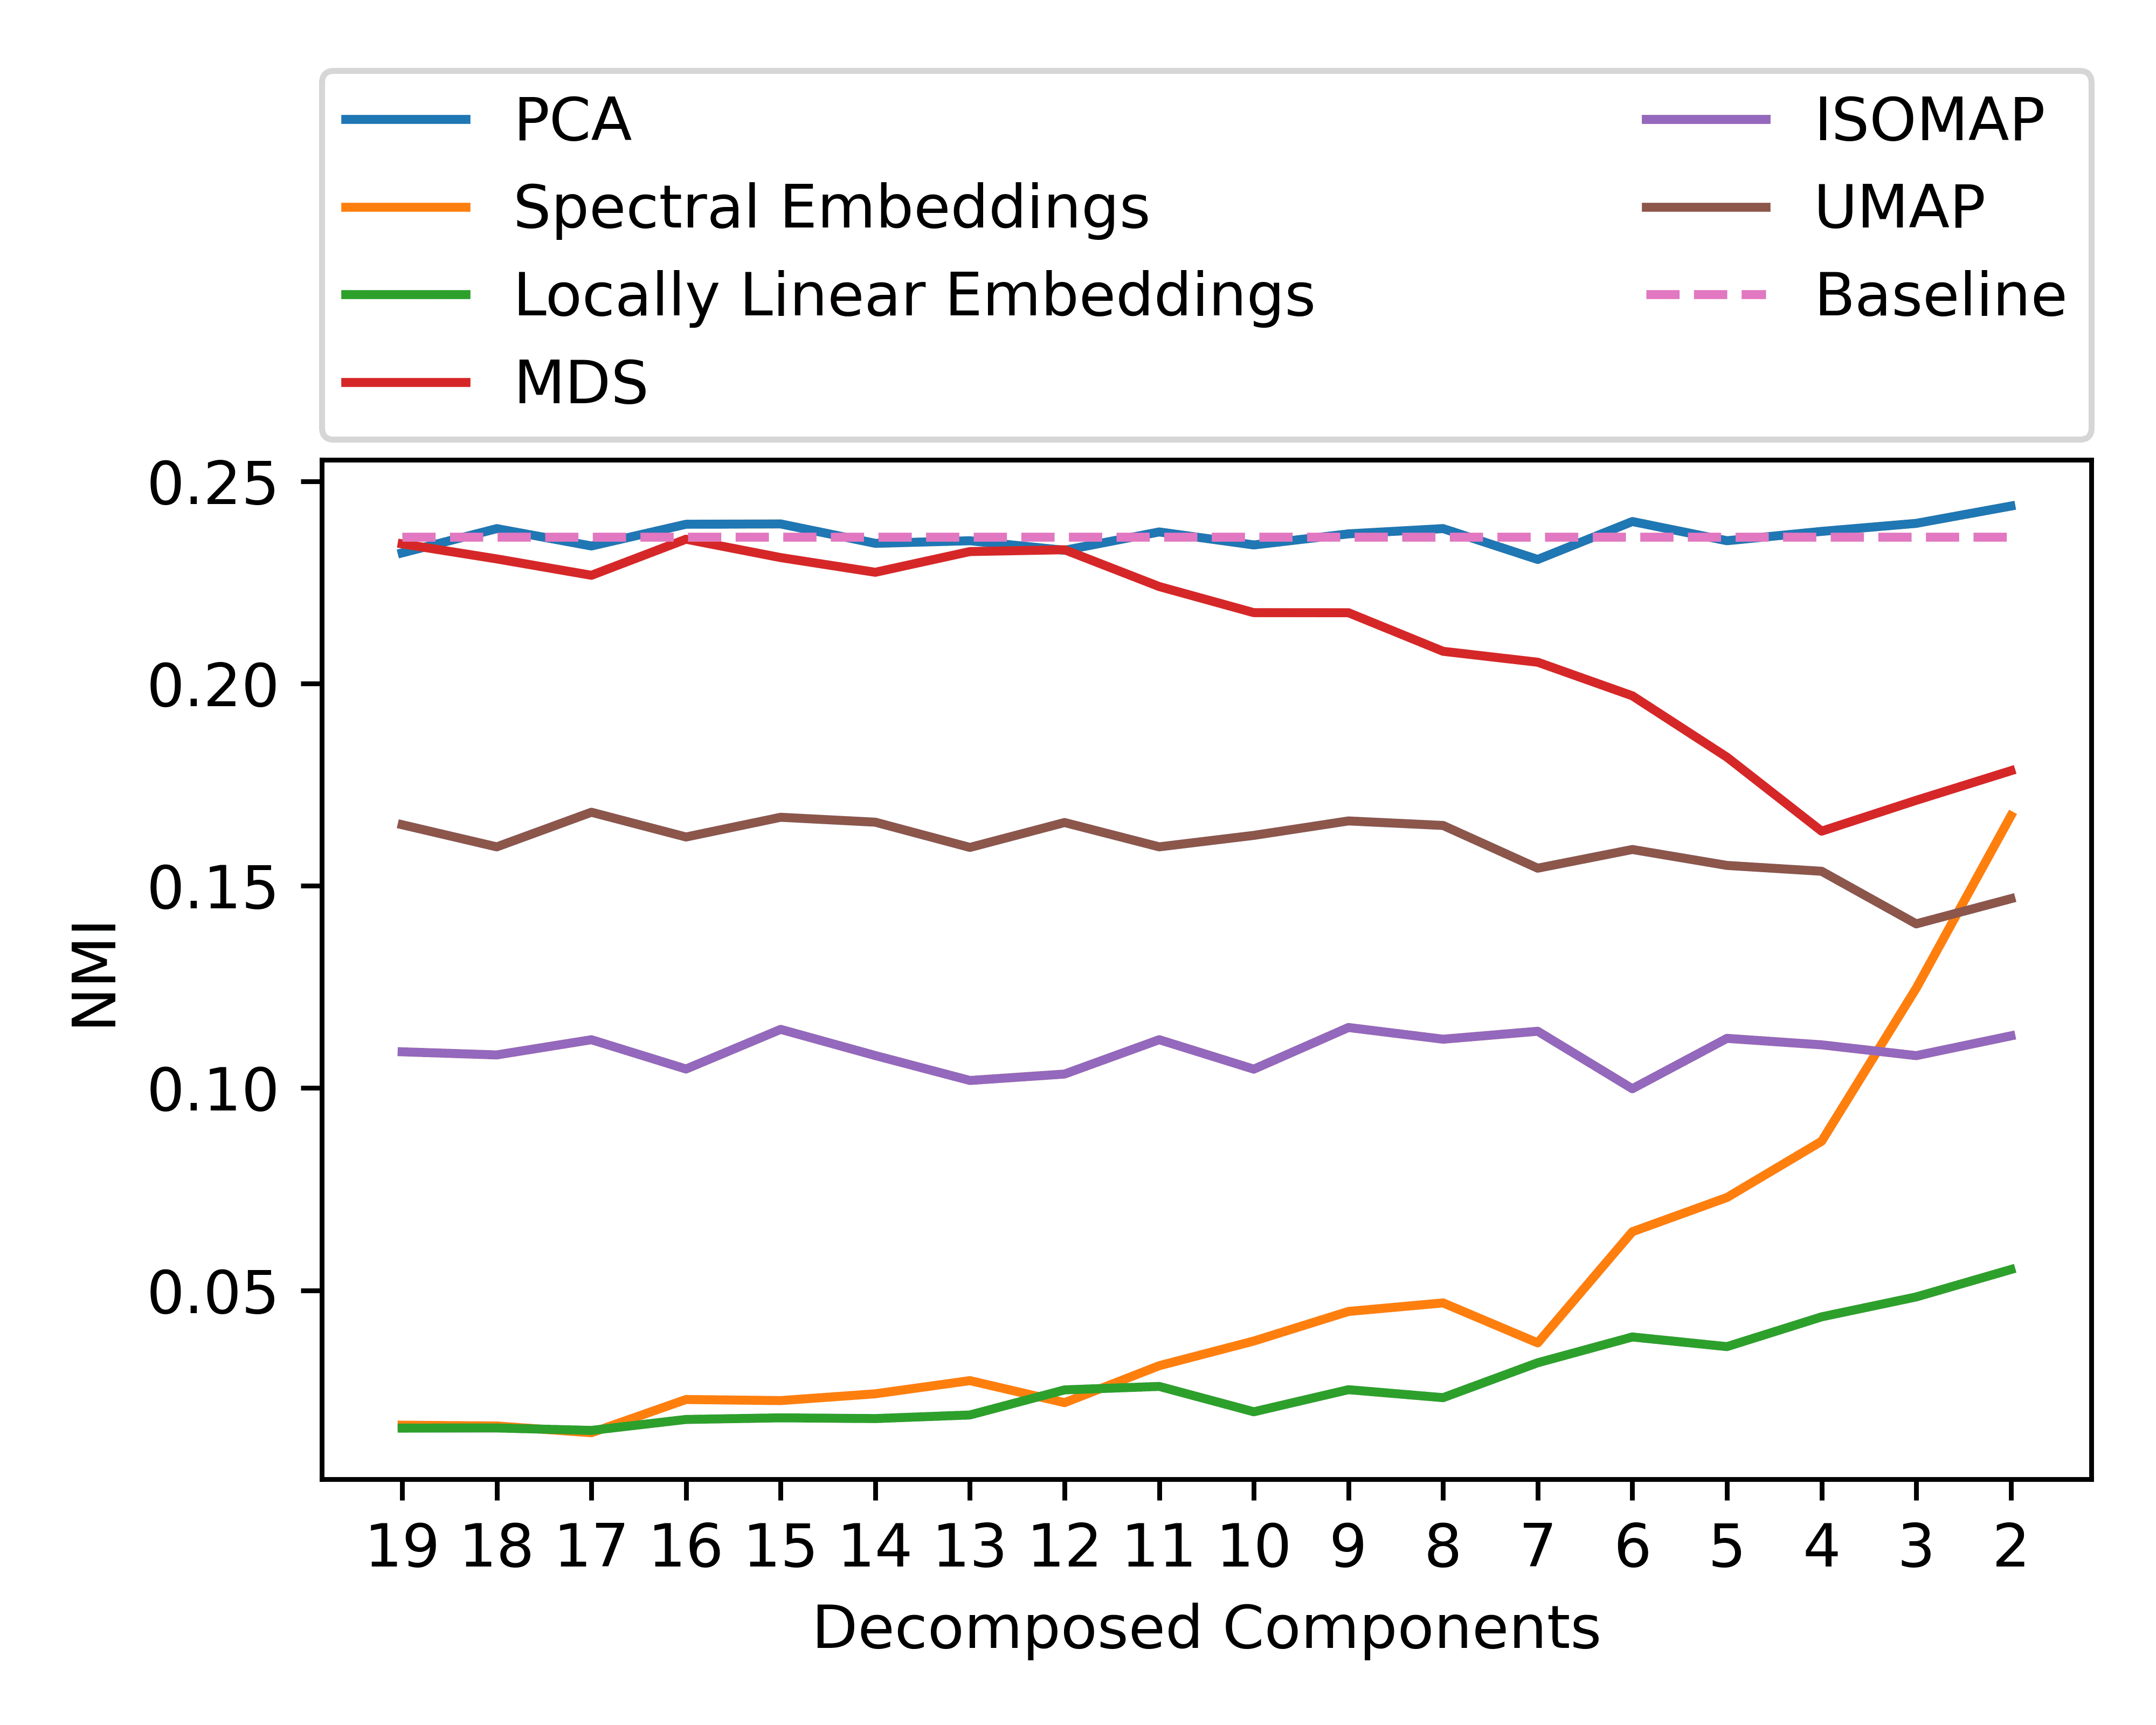
\includegraphics[width=0.48\linewidth]{images/charts/detailed_decomposition_metric_t_0.8_p_2_comparison_2_clusters_nmi.png}
                    \label{subfig:synthetic:t_0.8:dim_influence:nmi}
                }
                \subfigure[]{
                    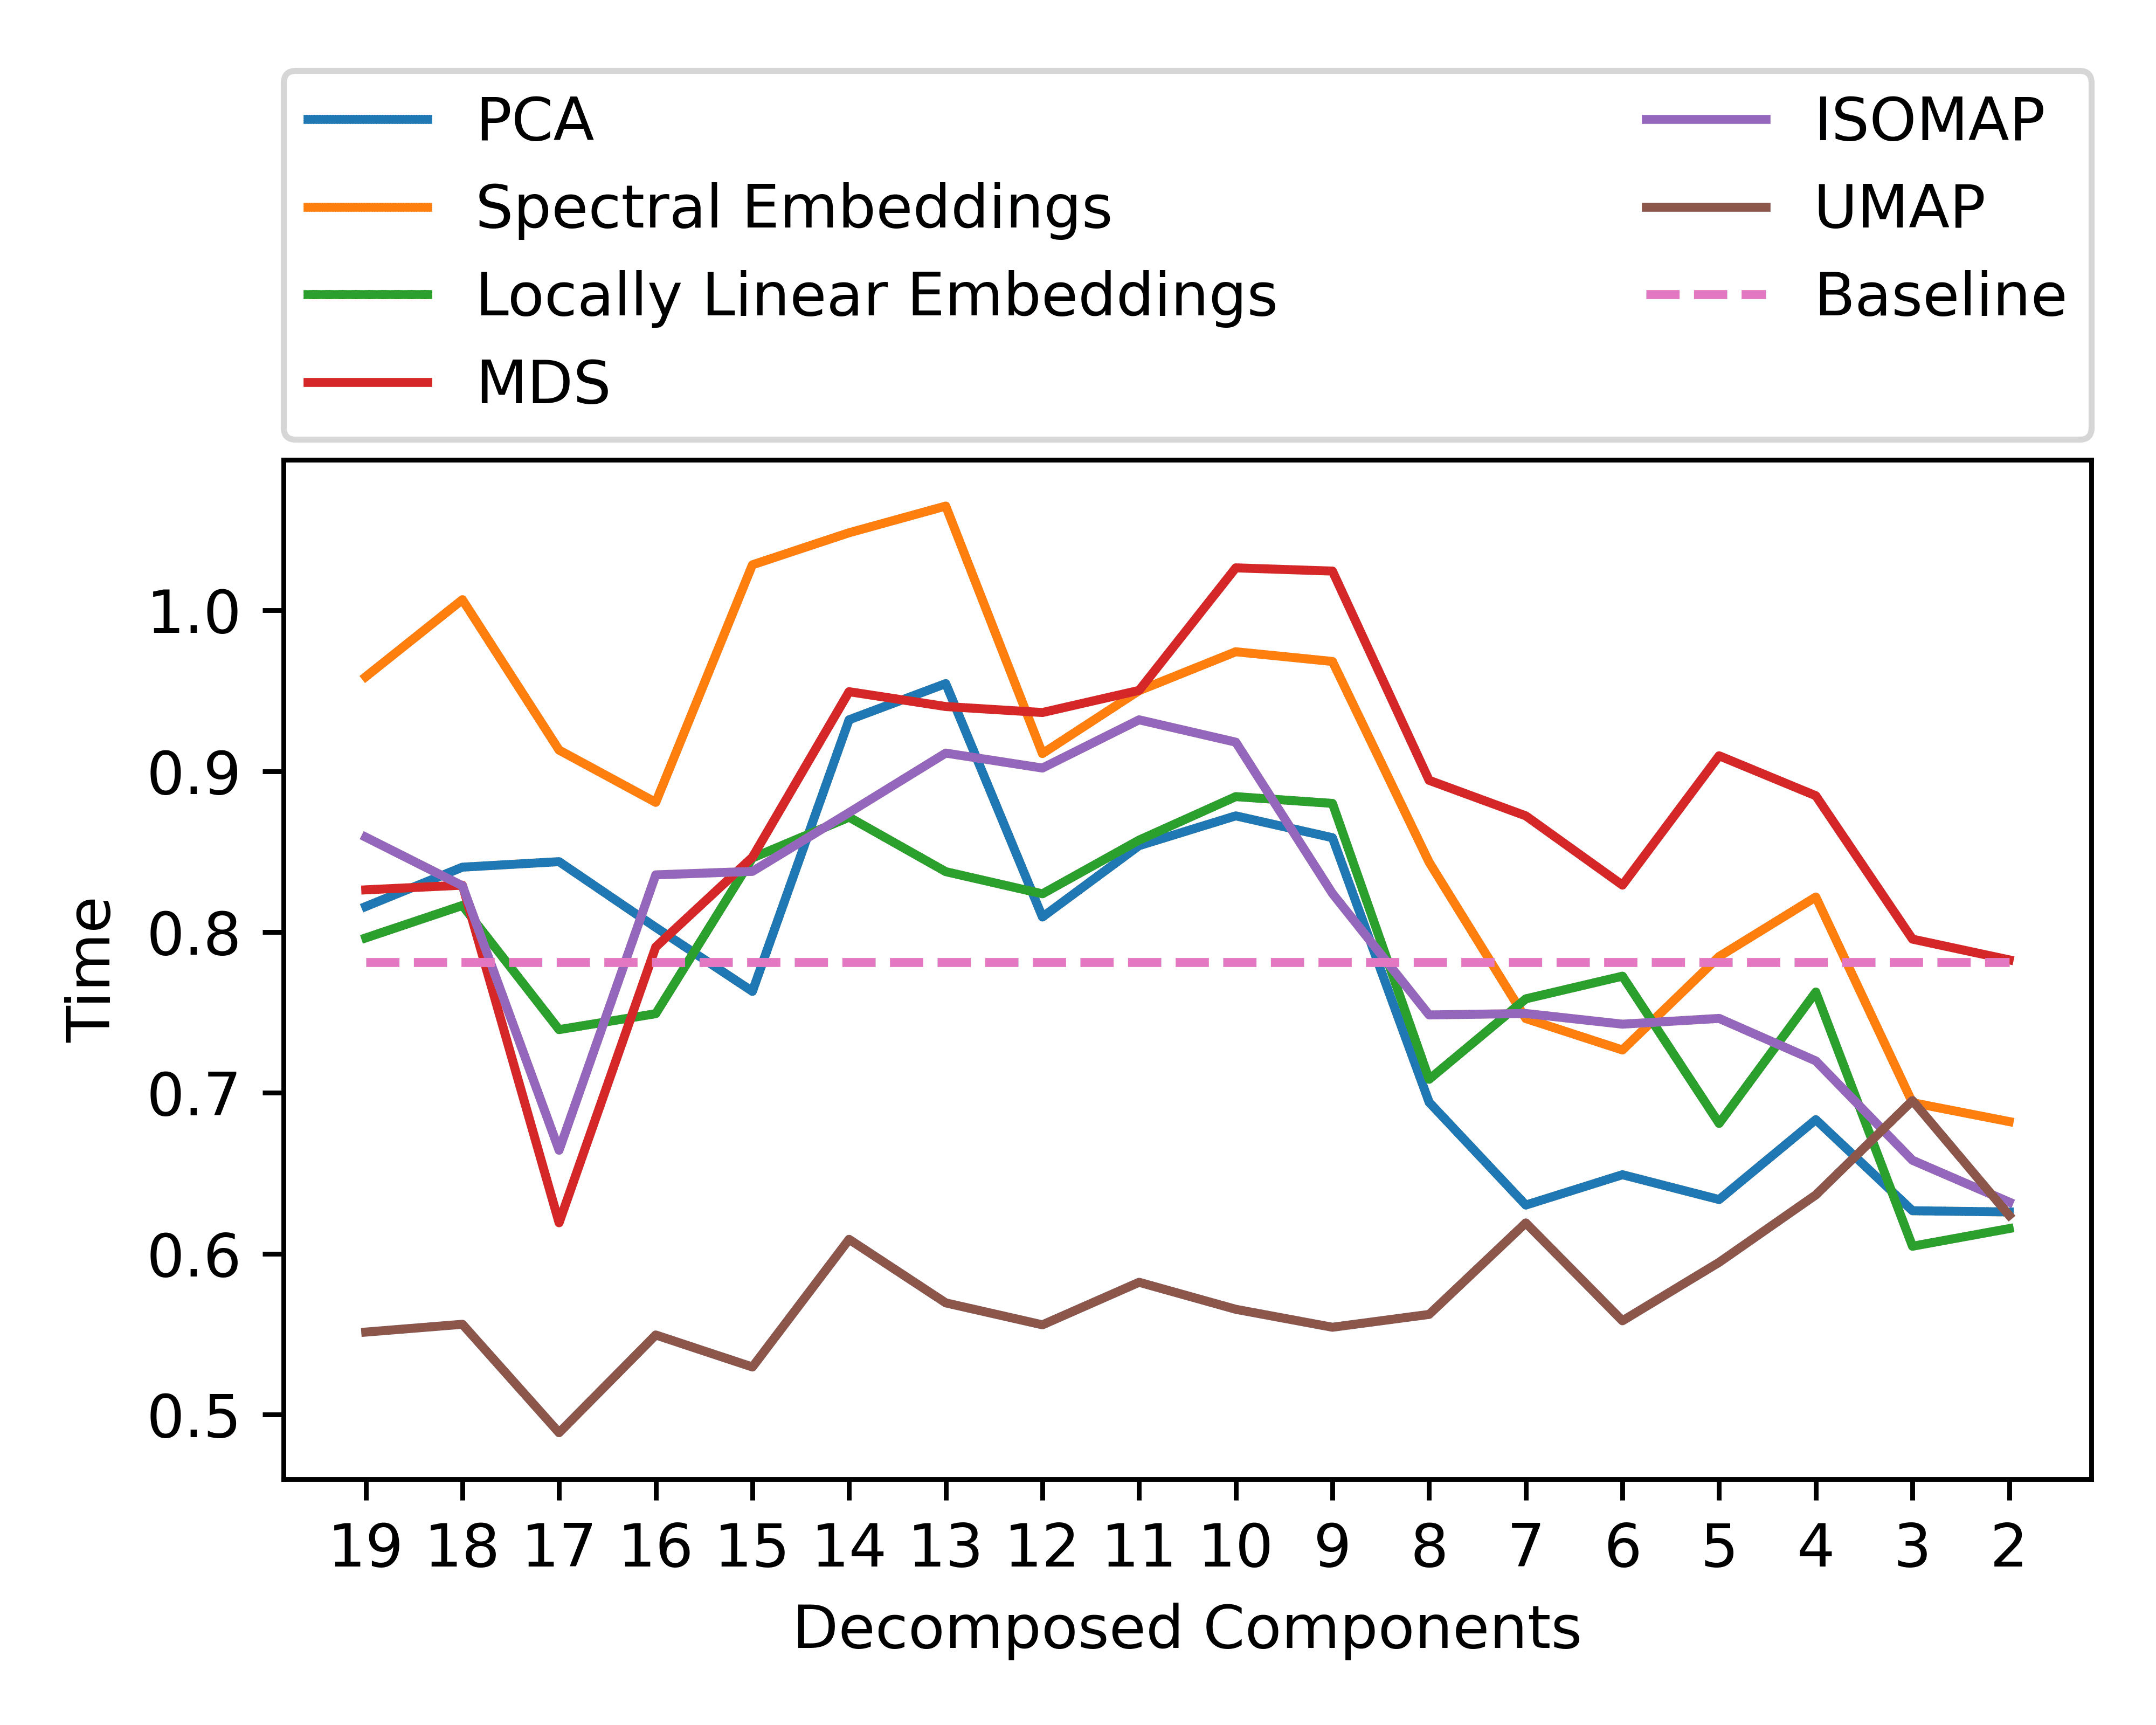
\includegraphics[width=0.48\linewidth]{images/charts/detailed_decomposition_metric_t_0.8_p_2_comparison_2_clusters_time.png}
                    \label{subfig:synthetic:t_0.8:dim_influence:time}
                }
                \caption{Анализ влияния размерности данных при различных методах снижения размерности на кластеризацию синтетического набора данных с параметром \(t = 0.8\). Линия Baseline -- результат работы алгоритма \kmeans{} без предварительного снижения размерности. Результаты для
                    \subref{subfig:synthetic:t_0.8:dim_influence:ami} AMI;
                    \subref{subfig:synthetic:t_0.8:dim_influence:ari} ARI;
                    \subref{subfig:synthetic:t_0.8:dim_influence:nmi} NMI, а также на время работы алгоритма \subref{subfig:synthetic:t_influence:time}.
                }
                \label{fig:synthetic:t_0.8:dim_influence}
            \end{figure}

            Таким образом, эксперимент подтвердил, что даже в условиях идеальной геометрии кластеров агрессивное снижение размерности способно существенно нарушить пространственную структуру, необходимую для корректной работы \kmeans{}. Наиболее устойчивыми к снижению размерности оказались методы PCA и MDS. Это подчеркивает важность выбора метода снижения размерности в зависимости от допустимой степени искажения данных при сохранении кластерной структуры.

        \subsubsection{Анализ поведения методов снижения кластеризации при сближении кластеров}
            В данной части экспериментов особое внимание уделяется анализу устойчивости и адаптивности различных методов снижения размерности в условиях, когда кластеры в данных становятся все менее различимыми -- то есть постепенно сближаются в пространстве признаков. Синтетическая модель, построенная как смесь нормальных распределений с контролируемым расстоянием между центрами кластеров, позволяет формализованно варьировать степень перекрытия кластеров с помощью параметра \(t\), не изменяя другие характеристики выборки.

            В условиях, когда \(t < 0\), центры кластеров максимально удаляются друг от друга без пересечений, что соответствует идеальному случаю для алгоритма \kmeans{}. По мере увеличения значения \(t\) до \(1\) центры притягиваются к общему центру масс, и границы между кластерами становятся все менее четкими, что моделирует реальные сценарии, в которых классы могут частично перекрываться. Такой подход позволяет объективно оценить, насколько методы понижения размерности сохраняют или теряют разделимость между группами при убывающем межкластерном расстоянии.

            Результаты экспериментов продемонстрированы на рисунке \ref{fig:synthetic:t_influence}, и показали высокую степень чувствительности к росту перекрытия кластеров.

            При анализе показателей AMI, ARI и NMI можно наблюдать устойчивое превосходство методов MDS, ISOMAP и UMAP на всех значениях параметра \(t\), особенно в областях, где кластеры хорошо разделены (\(t < 0.4\)). Эти методы демонстрируют почти идеальное восстановление кластерной структуры при низких значениях \(t\), что соответствует высокой степени отделенности кластеров. С увеличением \(t\) все методы, за исключением Spectral Embeddings и Locally Linear Embeddings (LLE), относительно стабильно теряют качество, однако сохраняют приемлемый уровень информативности вплоть до \(t \approx 0.6\). В то же время, методы Spectral и LLE показывают значительно худшие показатели на всех интервалах \(t\), демонстрируя явную нестабильность и уязвимость к изменению межкластерного расстояния.

            Особенно интересным является пик значений метрик (в районе \(t = 0.4\)) для Spectral и LLE, что может быть обусловлено локальным улучшением связности графов при частичном сближении кластеров. Однако после этого значения происходит резкое падение метрик, особенно AMI и NMI, указывающее на неспособность этих методов сохранять глобальную структуру данных при сильном перекрытии.

            С точки зрения времени выполнения, наименее ресурсоемким методом оказался UMAP, продемонстрировавший значительное снижение времени работы алгоритма кластеризации в пространстве меньшей размерности. Методы PCA, Spectral Embeddings, Locally Linear Embeddings, MDS, ISOMAP, напротив, показали увеличение времени работы при переходе в пространство меньше размерности (до 8 компонент), однако в пространствах размерности меньше 8, методы PCA, Locally Linear Embeddings, ISOMAP, продемонстрировали снижение времени работы алгоритма кластеризации, что делает их особенно предпочтительными для задач, требующих баланса между точностью и скоростью.

            Таким образом, в условиях постепенно сближающихся кластеров методы PCA, MDS и UMAP оказываются наиболее надежными как по качеству кластеризации, так и по вычислительным затратам. Методы Spectral Embeddings и Locally Linear Embeddings, напротив, показали нестабильное поведение и склонность к деградации качества при увеличении параметра \(t\).

            \begin{figure}[H]\centering
                \subfigure[]{
                    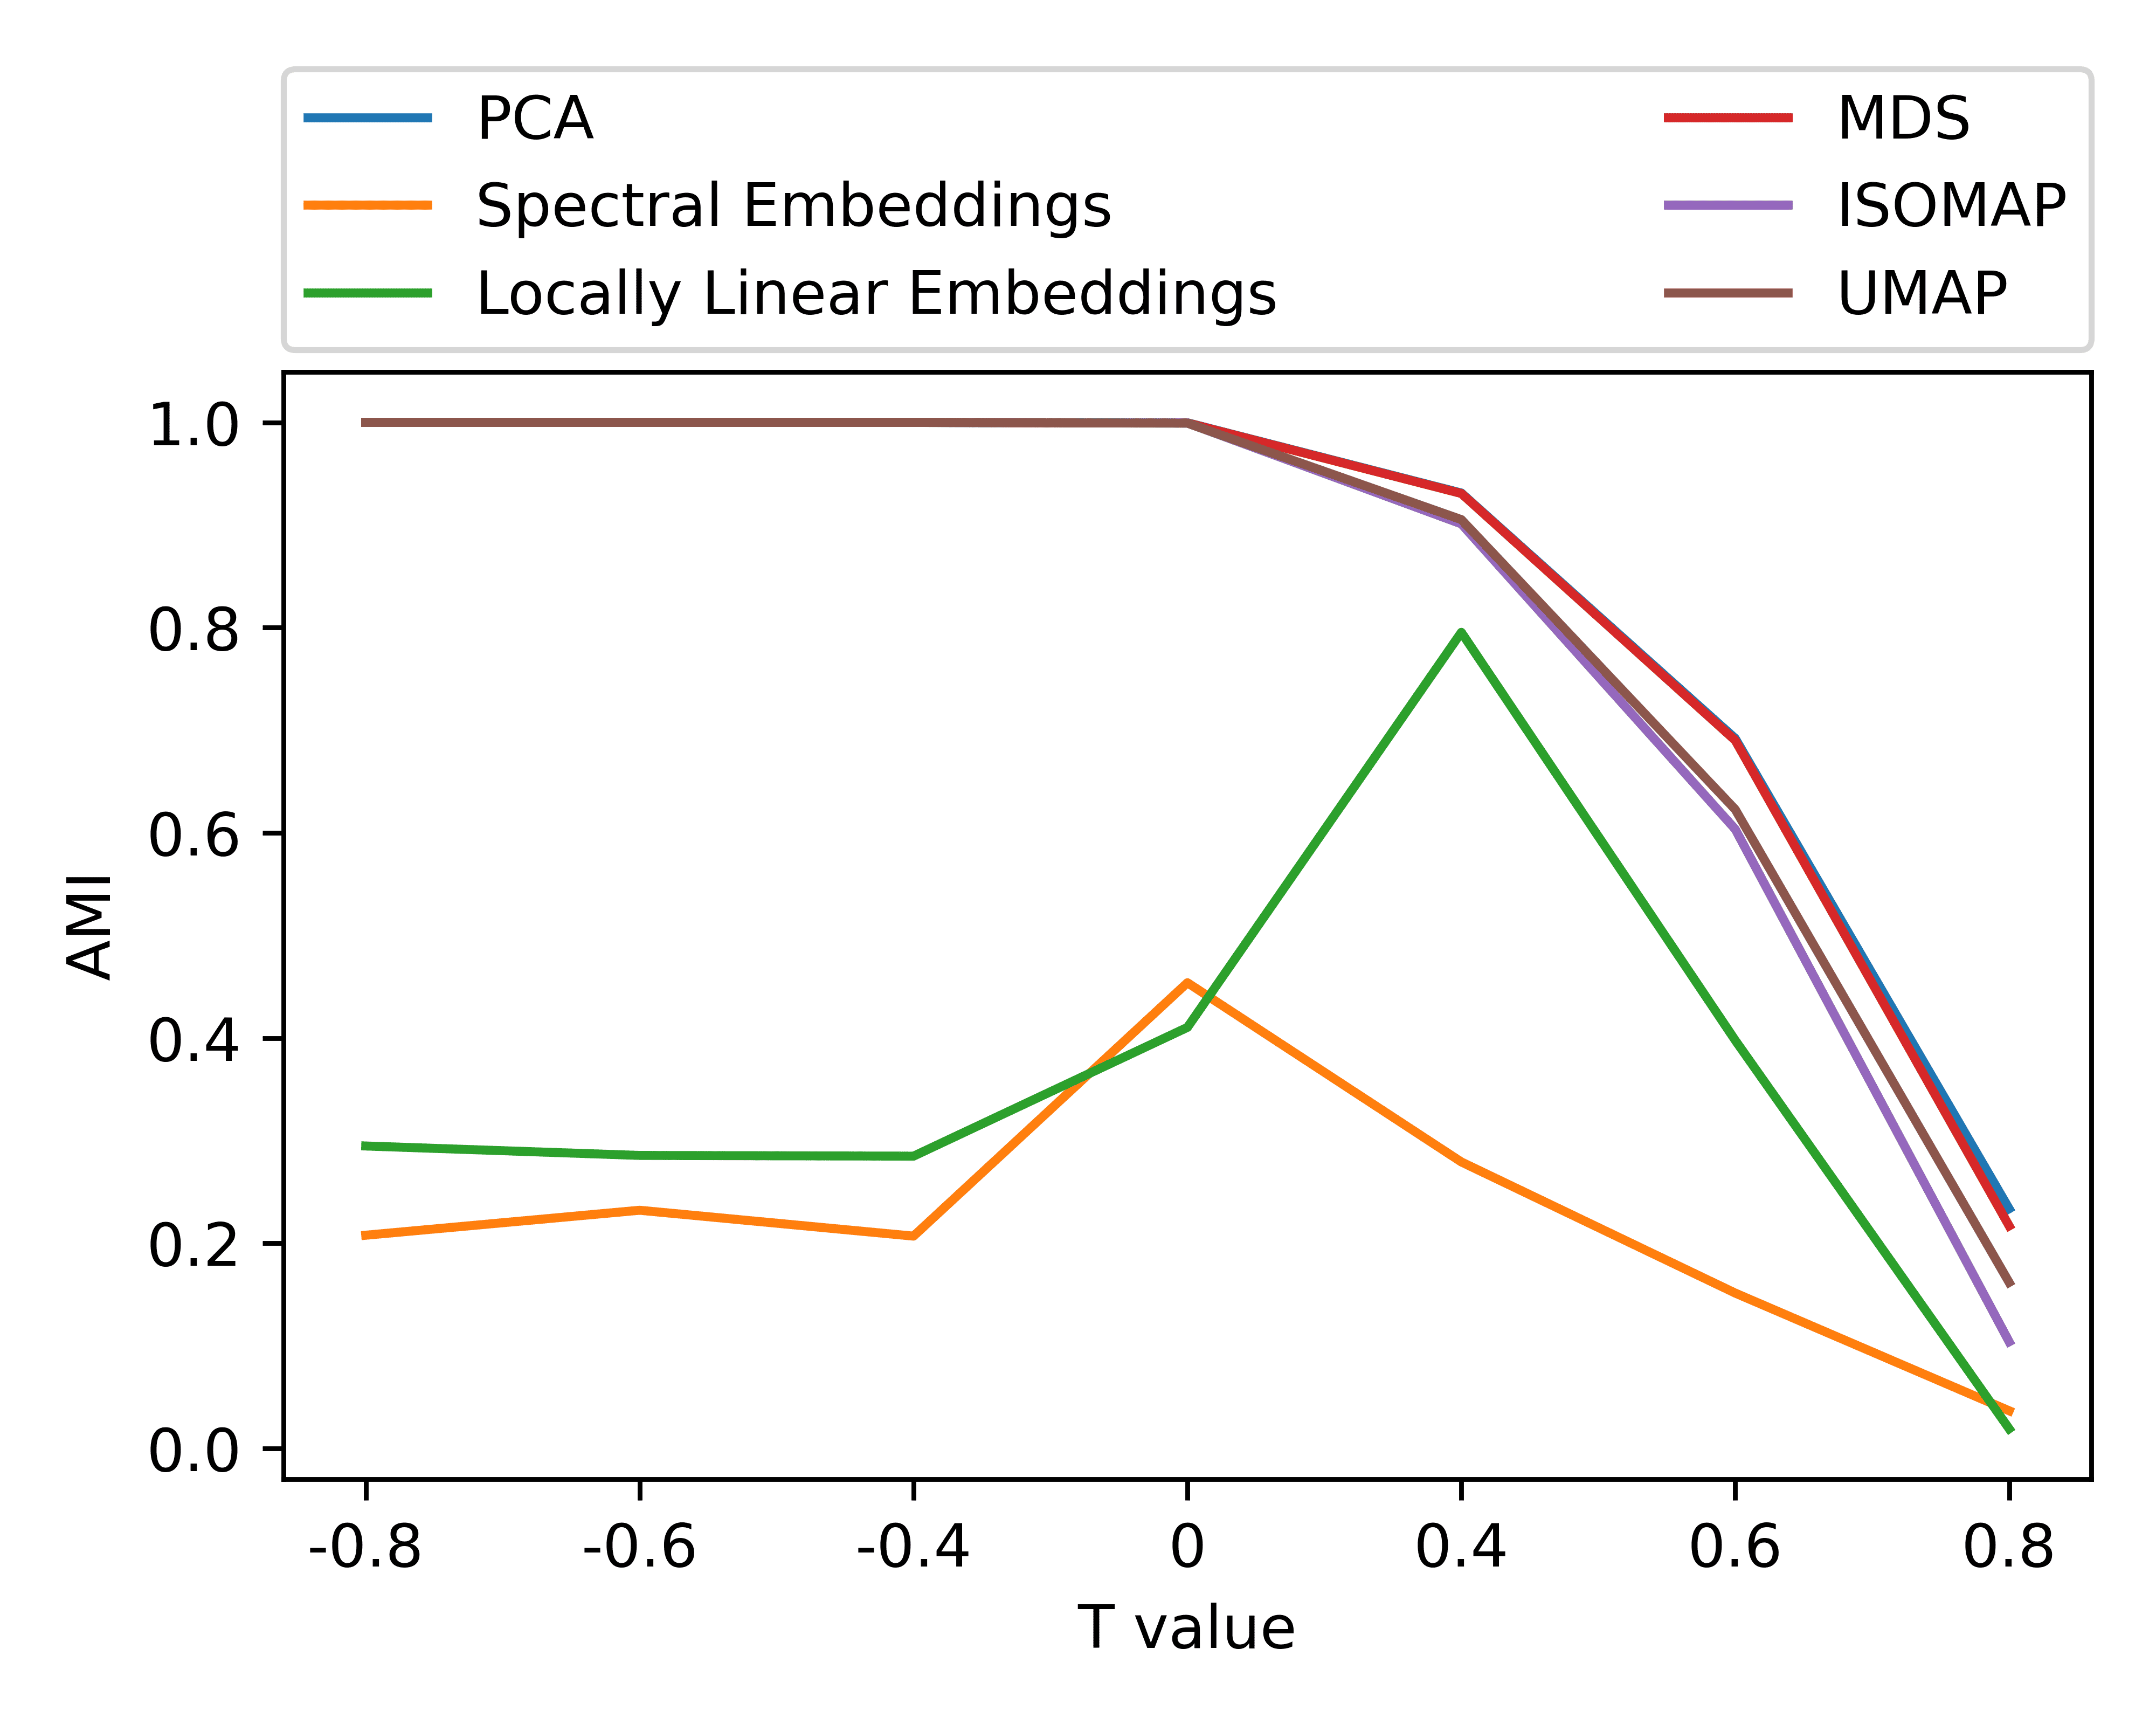
\includegraphics[width=0.48\linewidth]{images/charts/t_comparison_decomposition_20_p_2_comparison_2_clusters_ami.png}
                    \label{subfig:synthetic:t_influence:ami}
                }
                \subfigure[]{
                    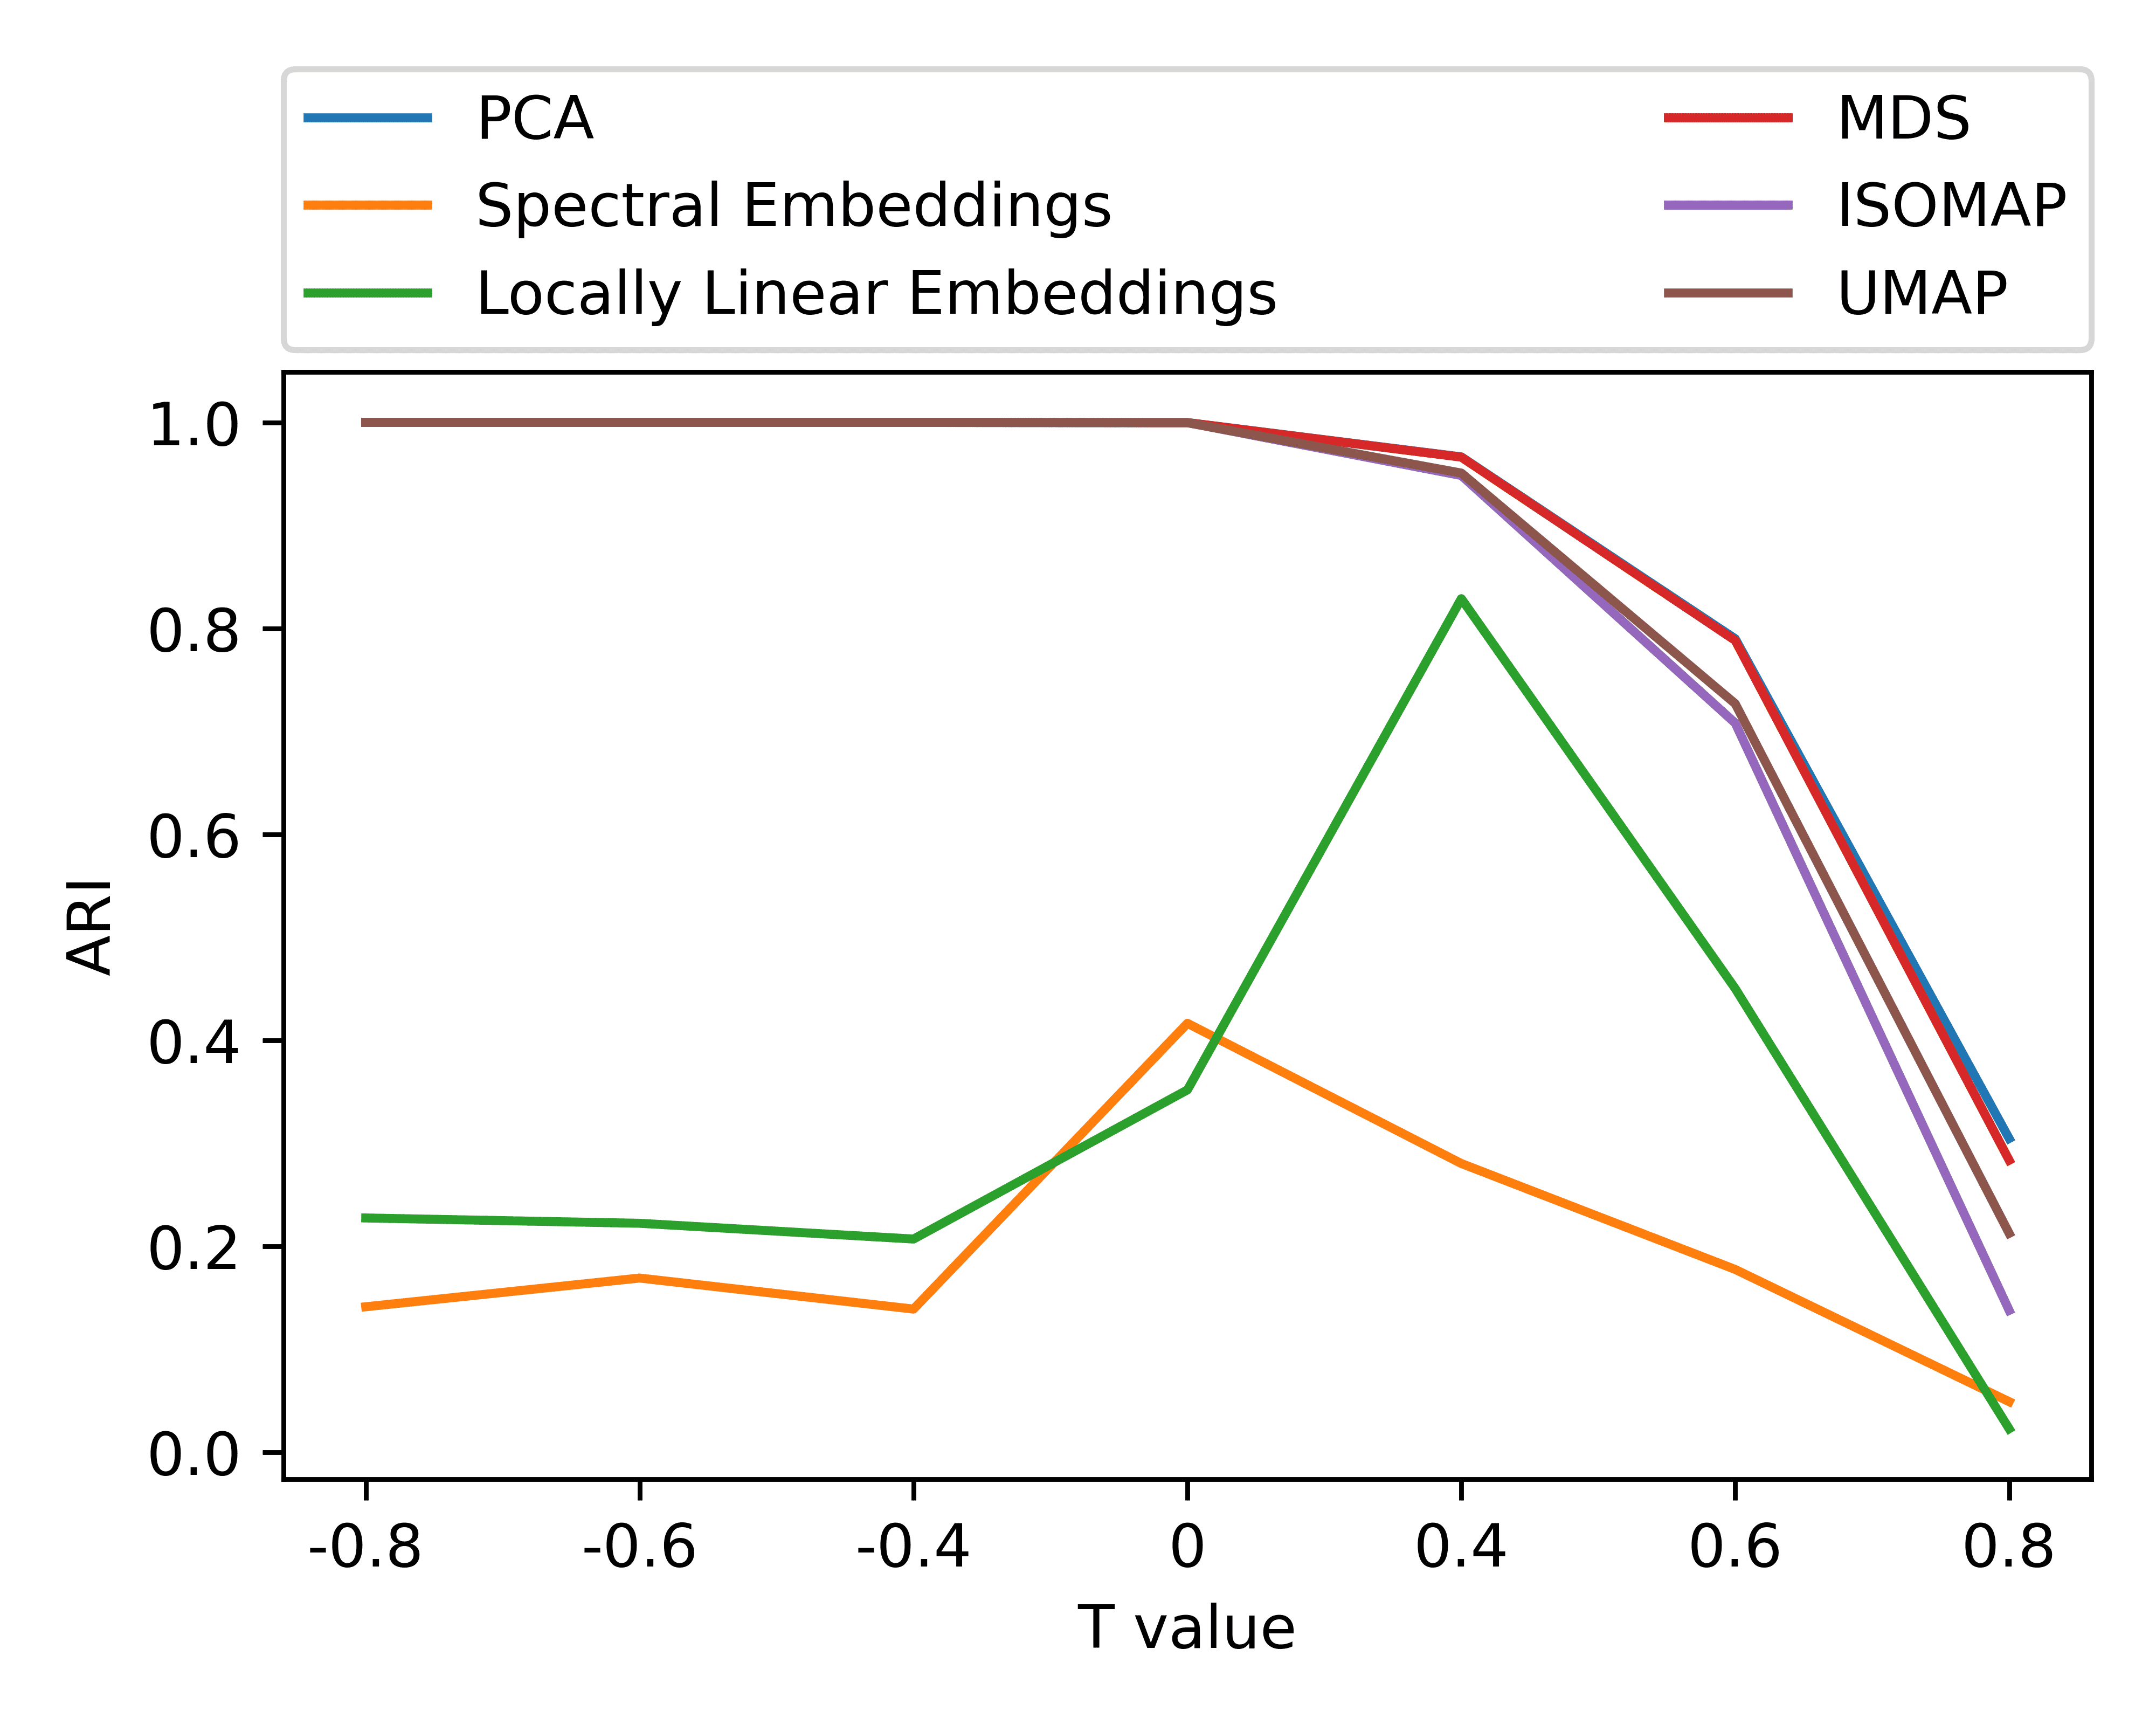
\includegraphics[width=0.48\linewidth]{images/charts/t_comparison_decomposition_20_p_2_comparison_2_clusters_ari.png}
                    \label{subfig:synthetic:t_influence:ari}
                }
                \subfigure[]{
                    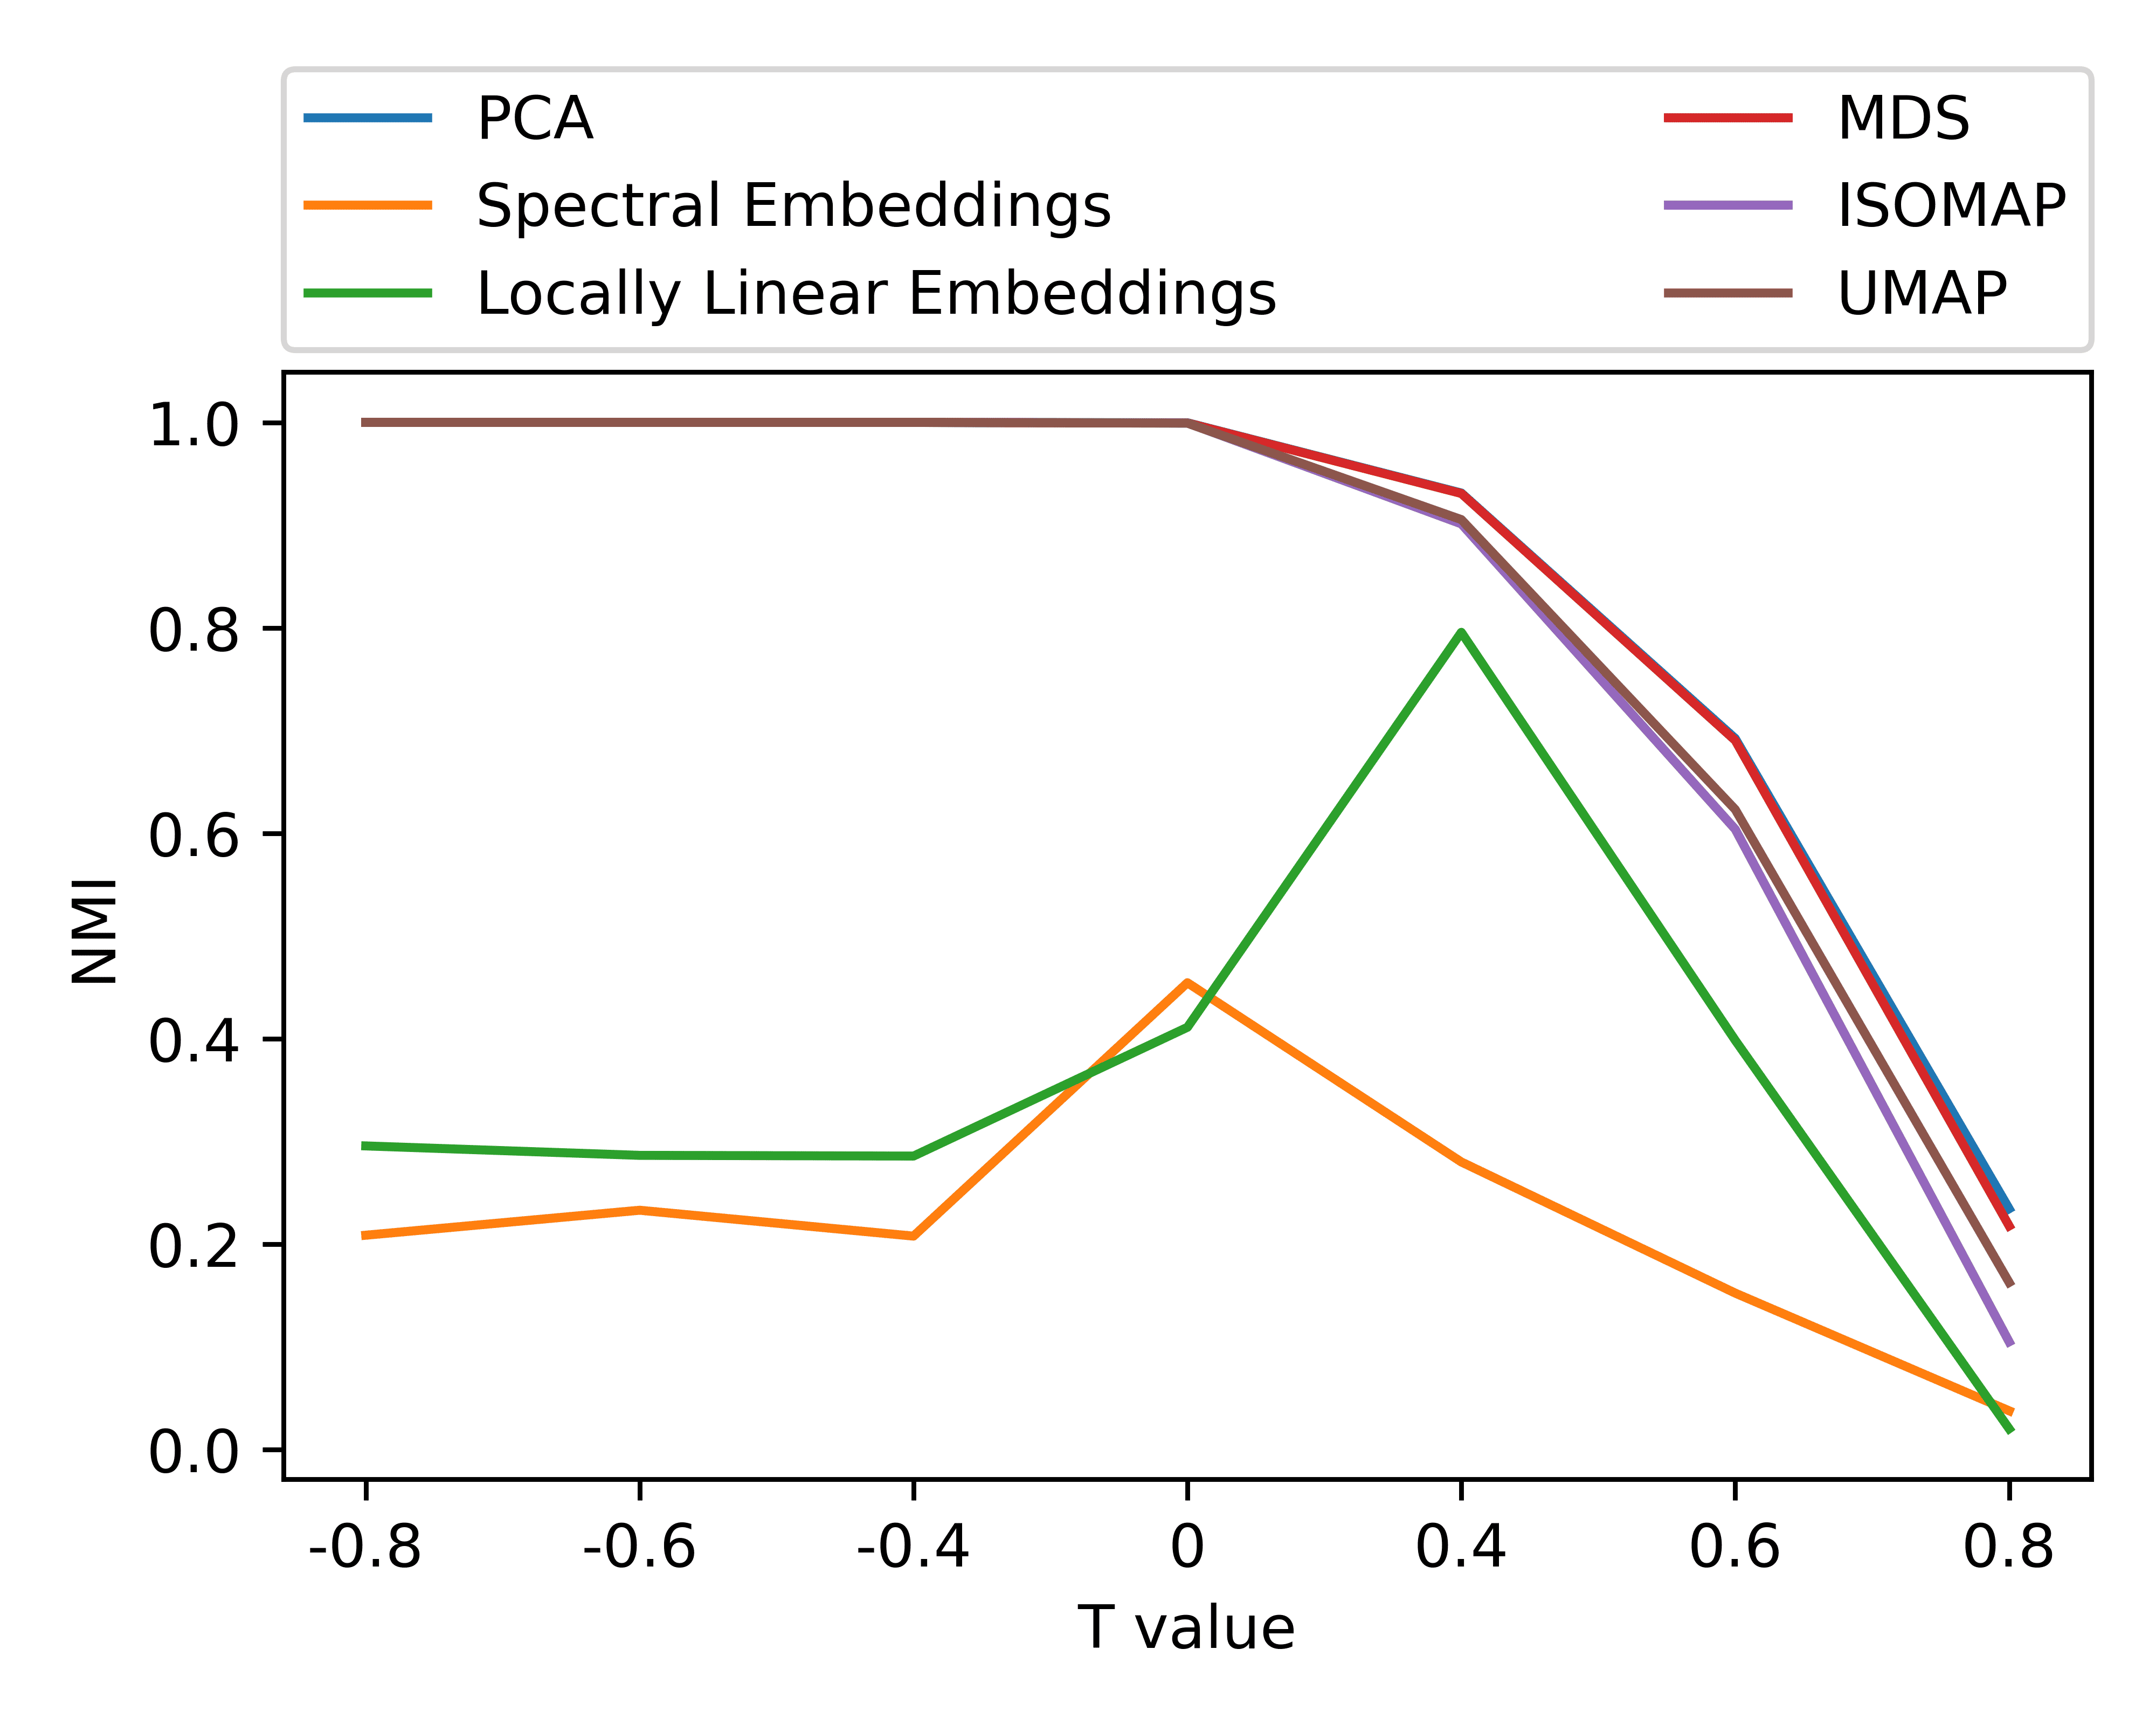
\includegraphics[width=0.48\linewidth]{images/charts/t_comparison_decomposition_20_p_2_comparison_2_clusters_nmi.png}
                    \label{subfig:synthetic:t_influence:nmi}
                }
                \subfigure[]{
                    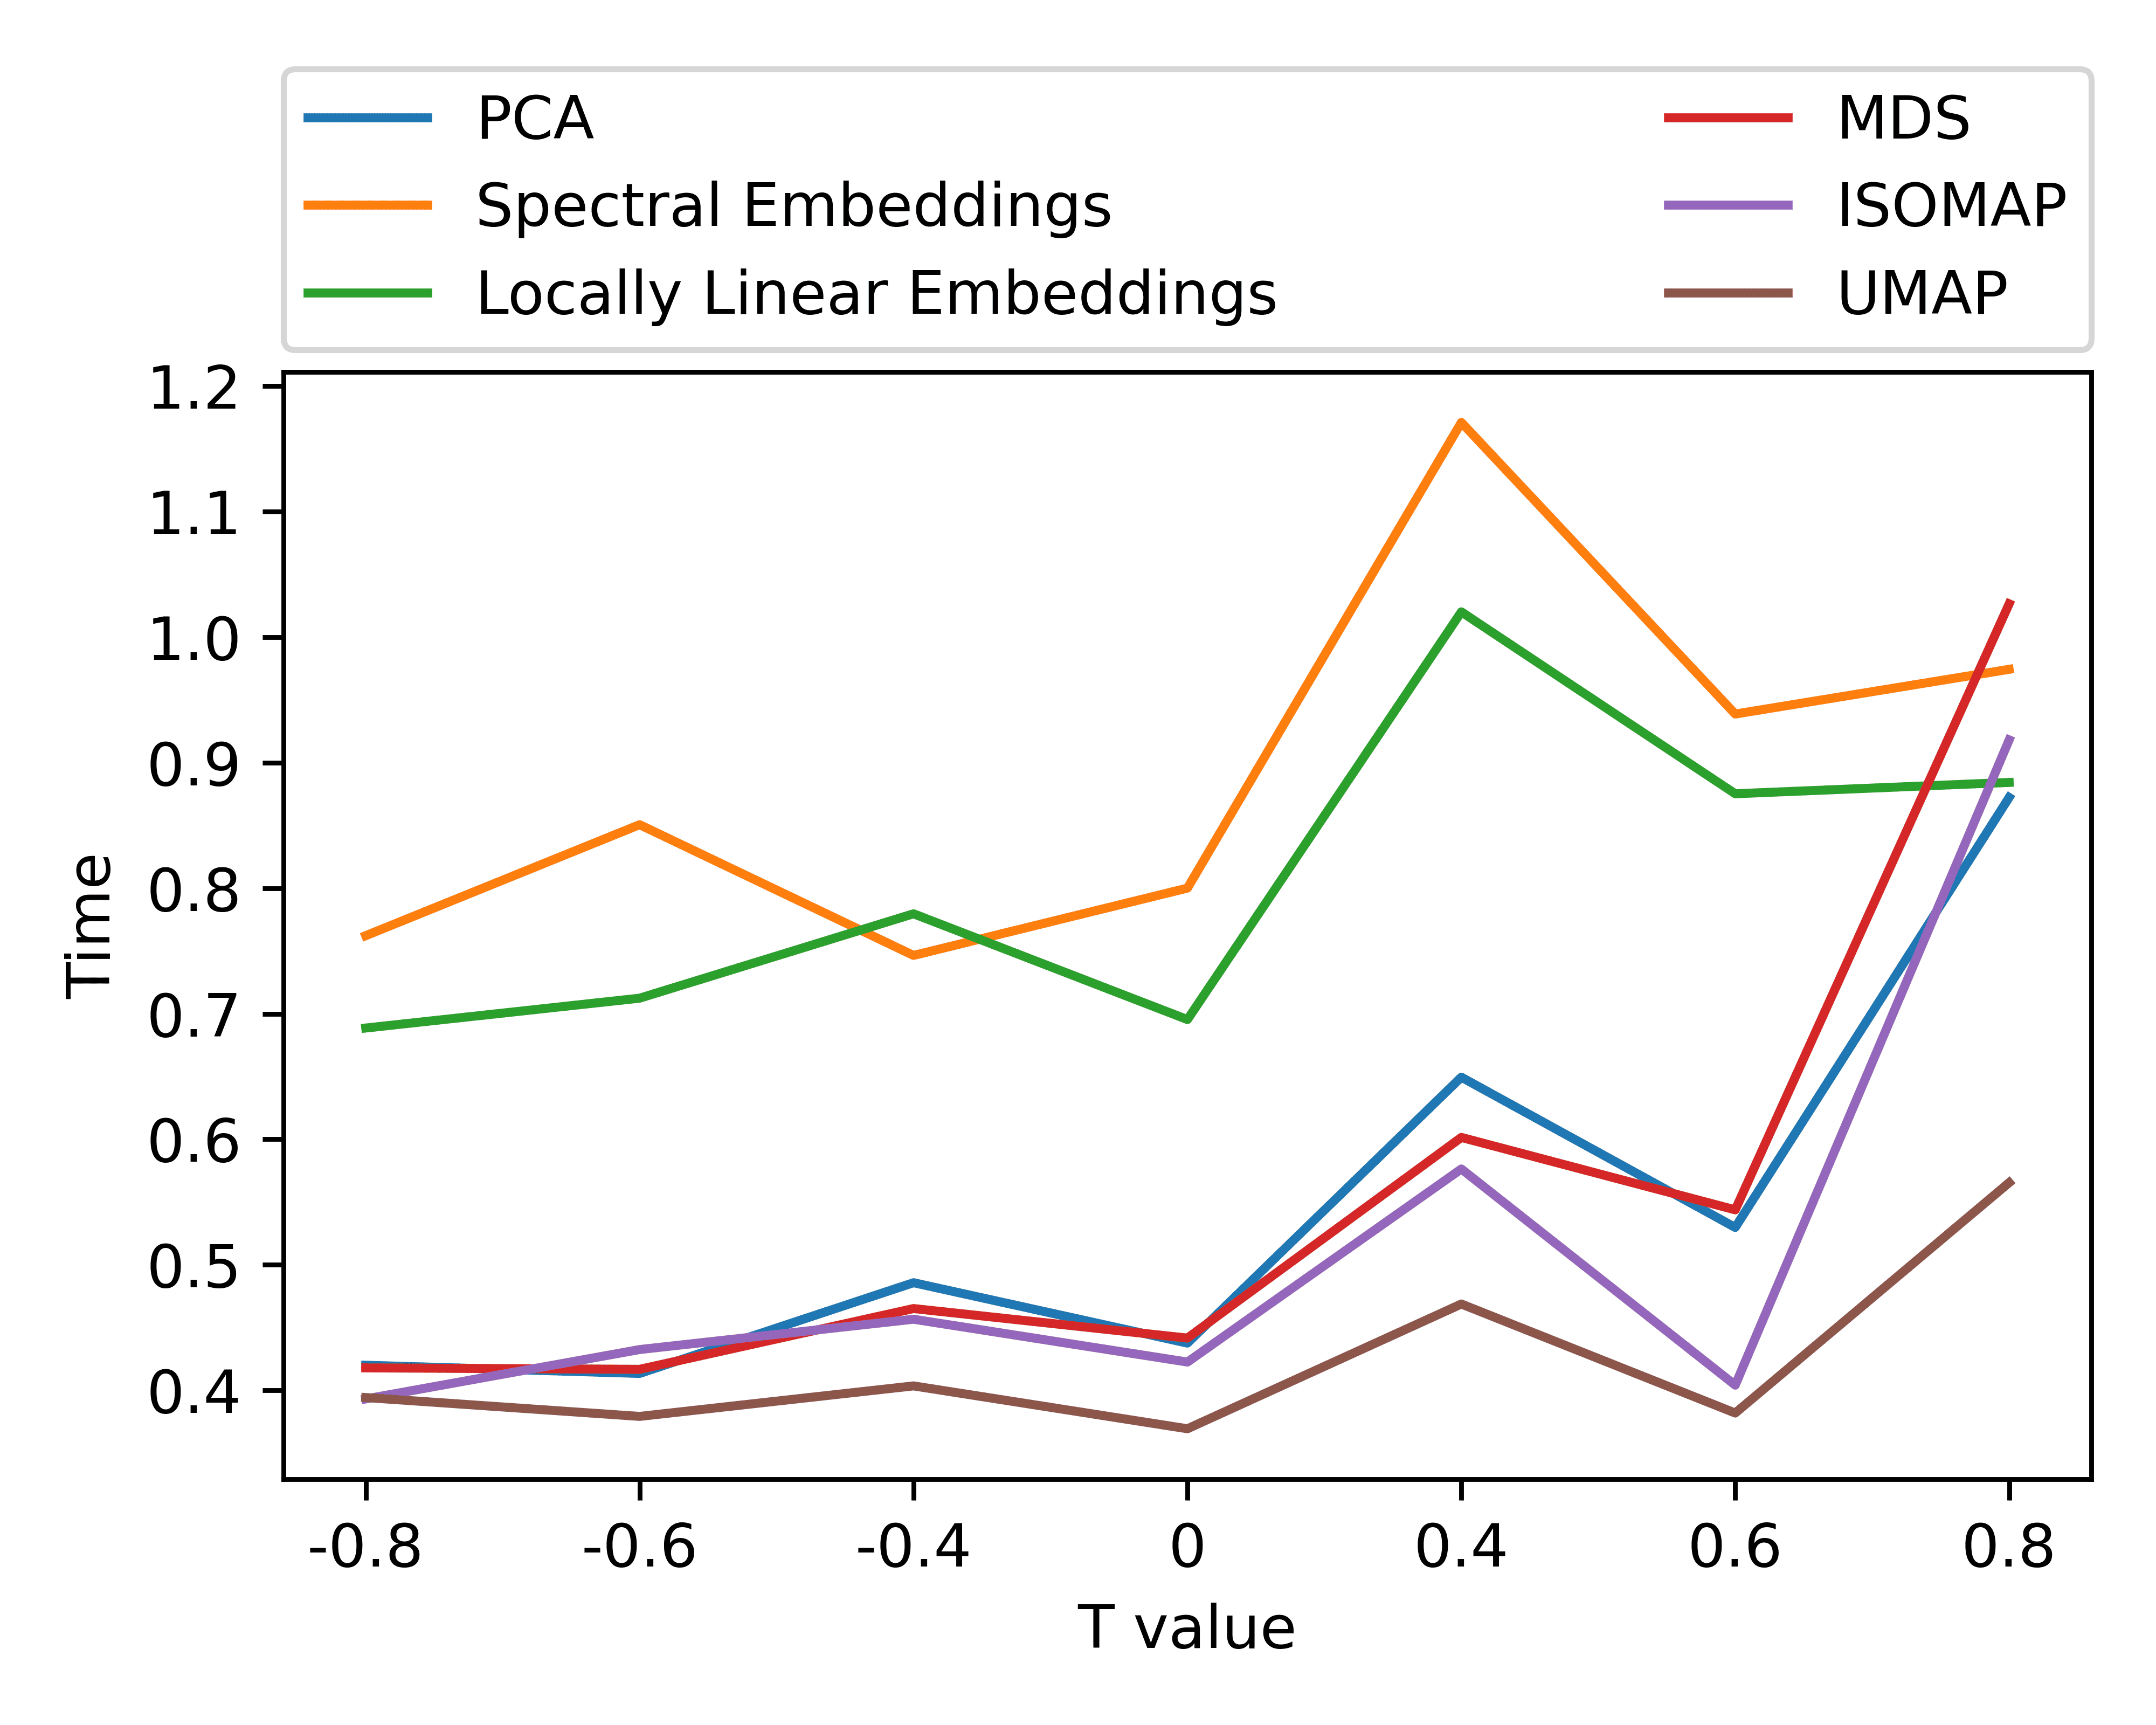
\includegraphics[width=0.48\linewidth]{images/charts/t_comparison_decomposition_20_p_2_comparison_2_clusters_time.png}
                    \label{subfig:synthetic:t_influence:time}
                }
                \caption{Анализ влияния различных методов снижения размерности данных на кластеризацию синтетического набора данных при сближении и отдалении центров кластеров. Результаты для
                    \subref{subfig:synthetic:t_influence:ami} AMI;
                    \subref{subfig:synthetic:t_influence:ari} ARI;
                    \subref{subfig:synthetic:t_influence:nmi} NMI, а также на время работы алгоритма \subref{subfig:synthetic:t_influence:time}.
                }
                \label{fig:synthetic:t_influence}
            \end{figure}

            Таким образом, анализ на синтетических данных подтвердил, что эффективность методов снижения размерности сильно зависит от геометрии и плотности кластеров. Это подчеркивает необходимость адаптивного выбора метода снижения размерности в зависимости от ожидаемой сложности кластерной структуры в данных.

    \subsection{Эксперименты на реальных данных}

        Также предложенный подход был исследован на реальных данных. Для этого было решено использовать несколько стандартных наборов данных:

        \begin{itemize}
            \item Breast Cancer \cite{dataset:breastcancer},
            \item Digits \cite{dataset:digits},
            \item Wine \cite{dataset:wine}.
        \end{itemize}

        \subsubsection{Результаты алгоритма на наборе данных Breast Cancer}
            Breast Cancer -- это стандартный набор данных для бинарной классификации, часто используемый в задачах медицинской диагностики. Данные содержат результаты измерений опухолей молочной железы, полученные при помощи тонкоигольной аспирационной биопсии (FNA). Каждая запись включает характеристики клеточных ядер, такие как радиус, текстура, периметр и другие морфологические признаки.

            \begin{table}[H]
                \centering
                \caption{Характеристики набора данных Breast Cancer.}
                \begin{tabular}{ccc}
                    \toprule
                    Число классов & Число объектов & Размерность пространства \\
                    \midrule
                    2 & 569 & 30 \\
                    \bottomrule
                \end{tabular}
            \end{table}

            Набор данных Breast Cancer представляет собой матрицу размерностью 569x30, где каждая строка соответствует отдельному образцу опухоли, а каждый столбец содержит числовое значение одного из диагностических признаков. Целевая переменная указывает на доброкачественность (benign) или злокачественность (malignant) новообразования. Данные часто используются для обучения моделей машинного обучения, направленных на автоматизацию диагностики рака молочной железы.

            \begin{figure}[H]\centering
                \subfigure[]{
                    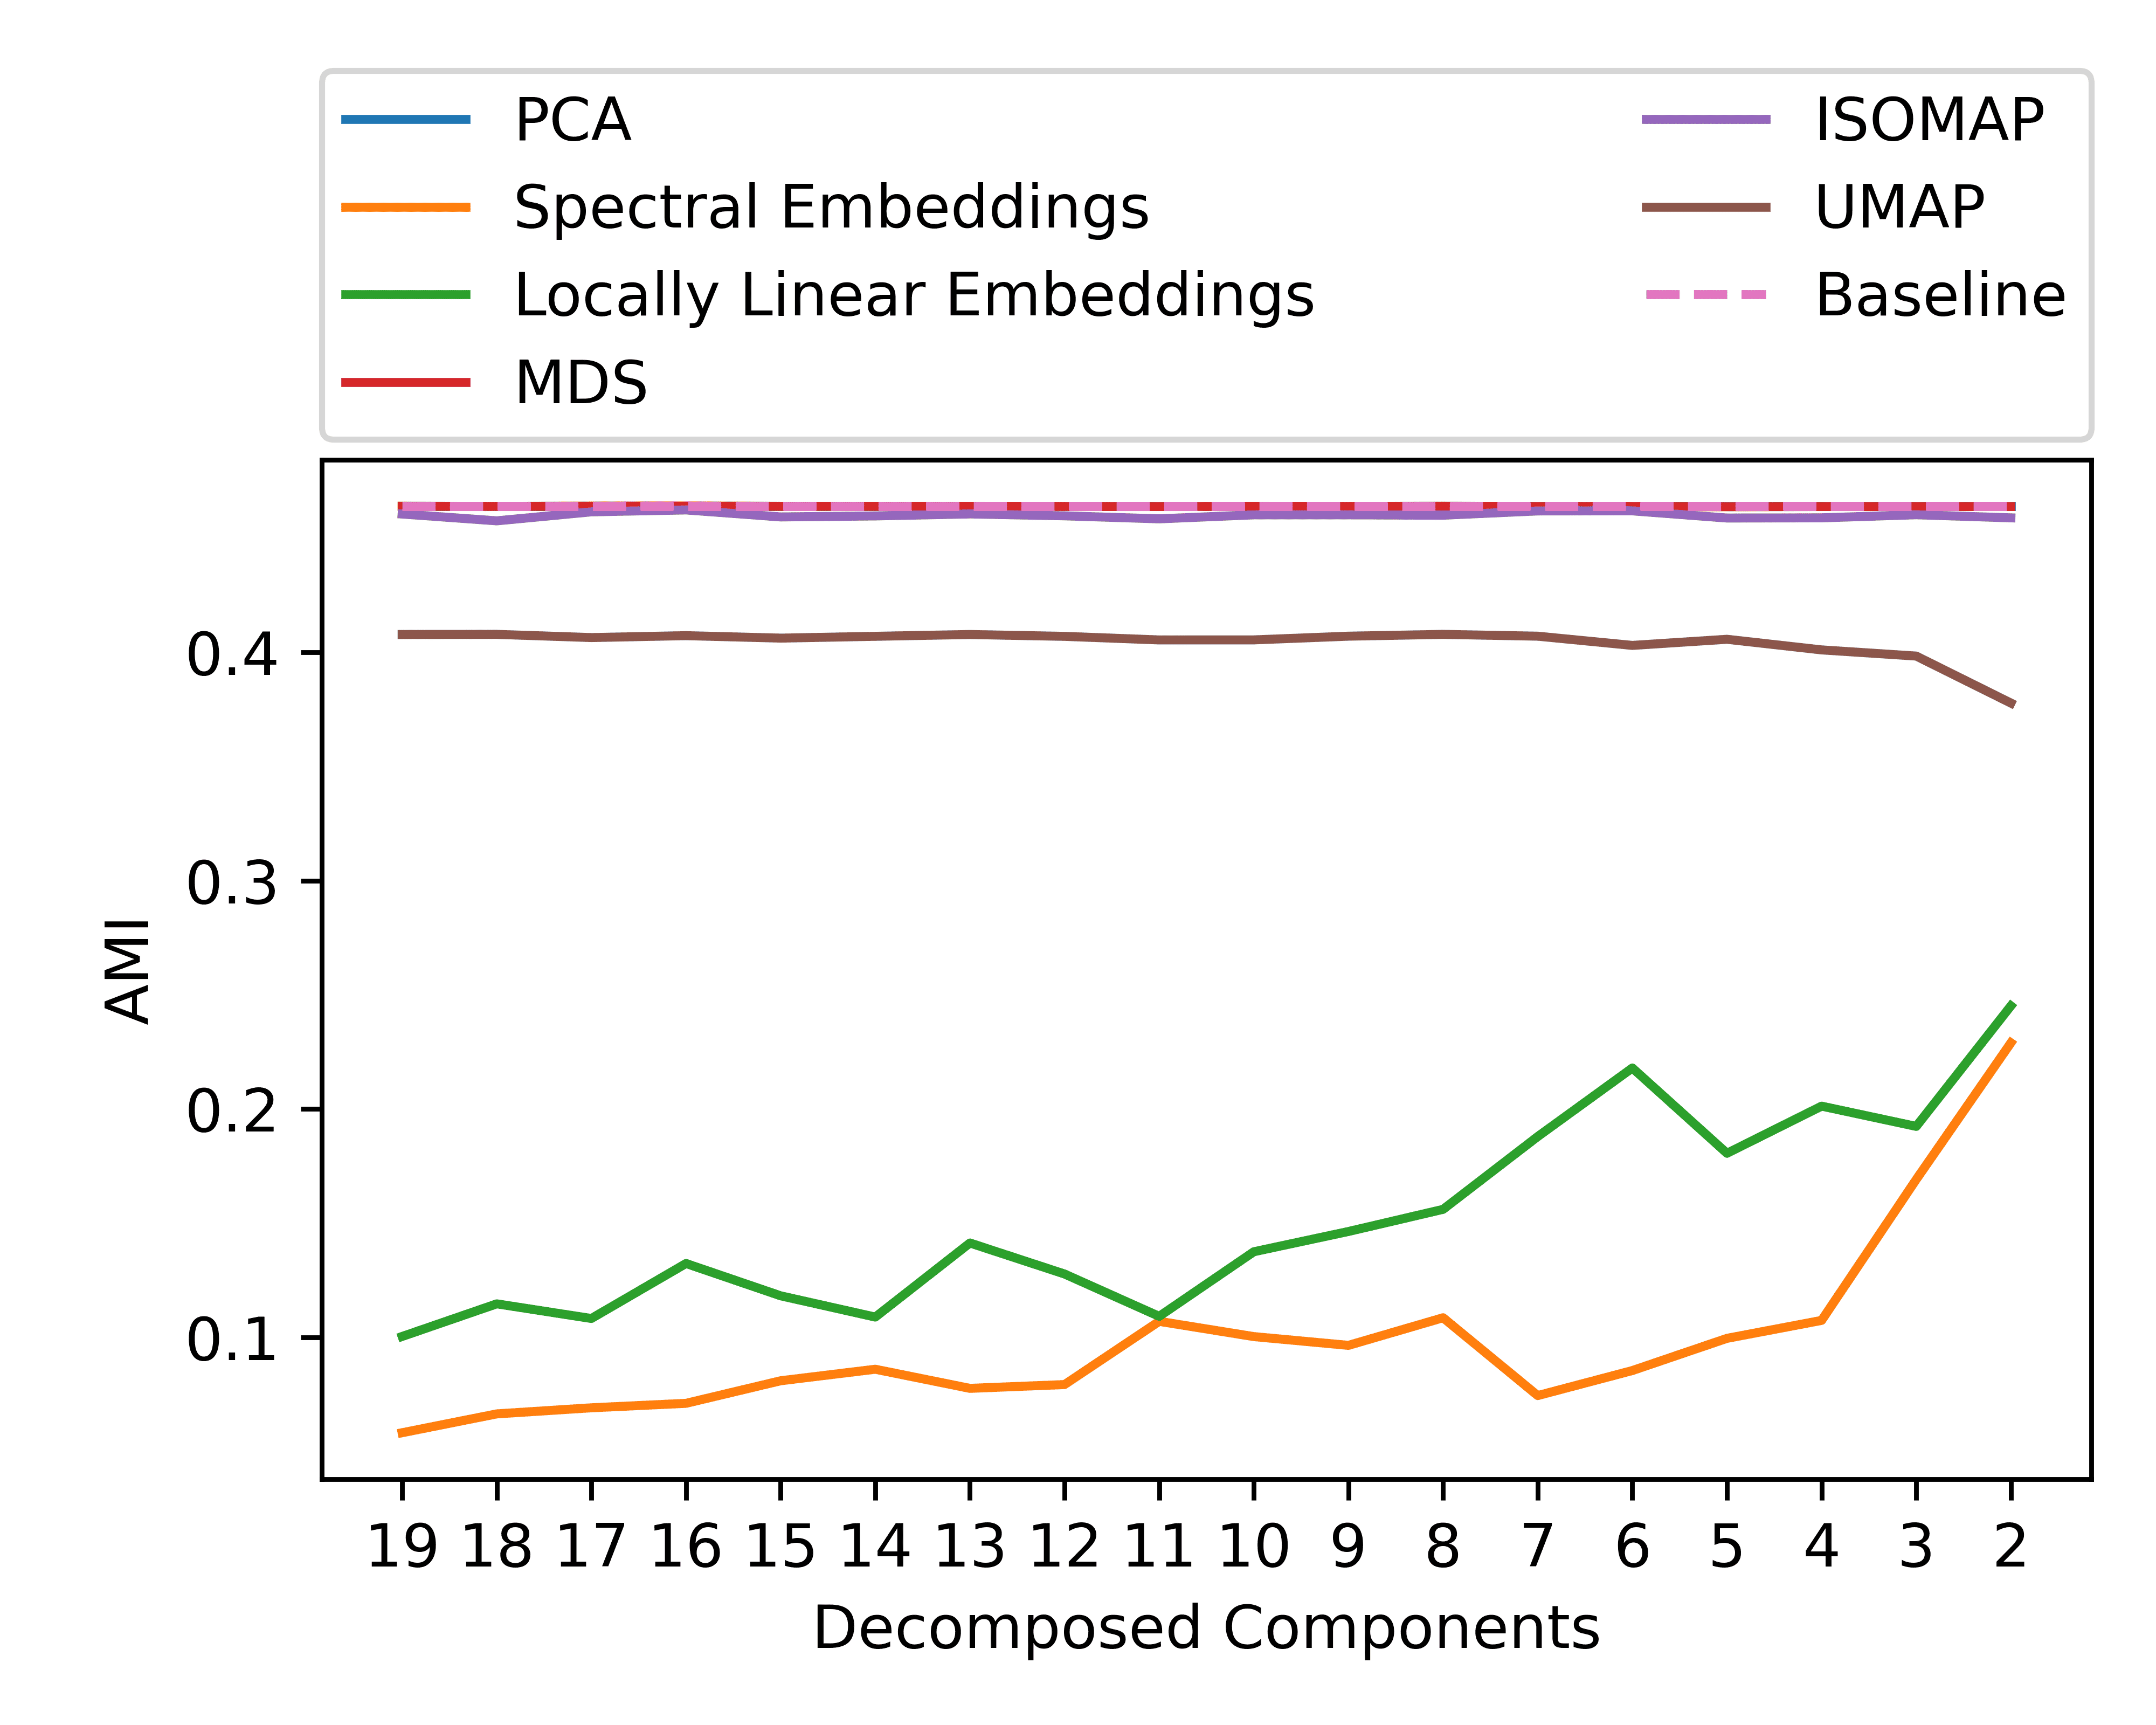
\includegraphics[width=0.48\linewidth]{images/charts_real/real_data_breast_cancer_ami.png}
                    \label{subfig:breast_cancer:ami}
                }
                \subfigure[]{
                    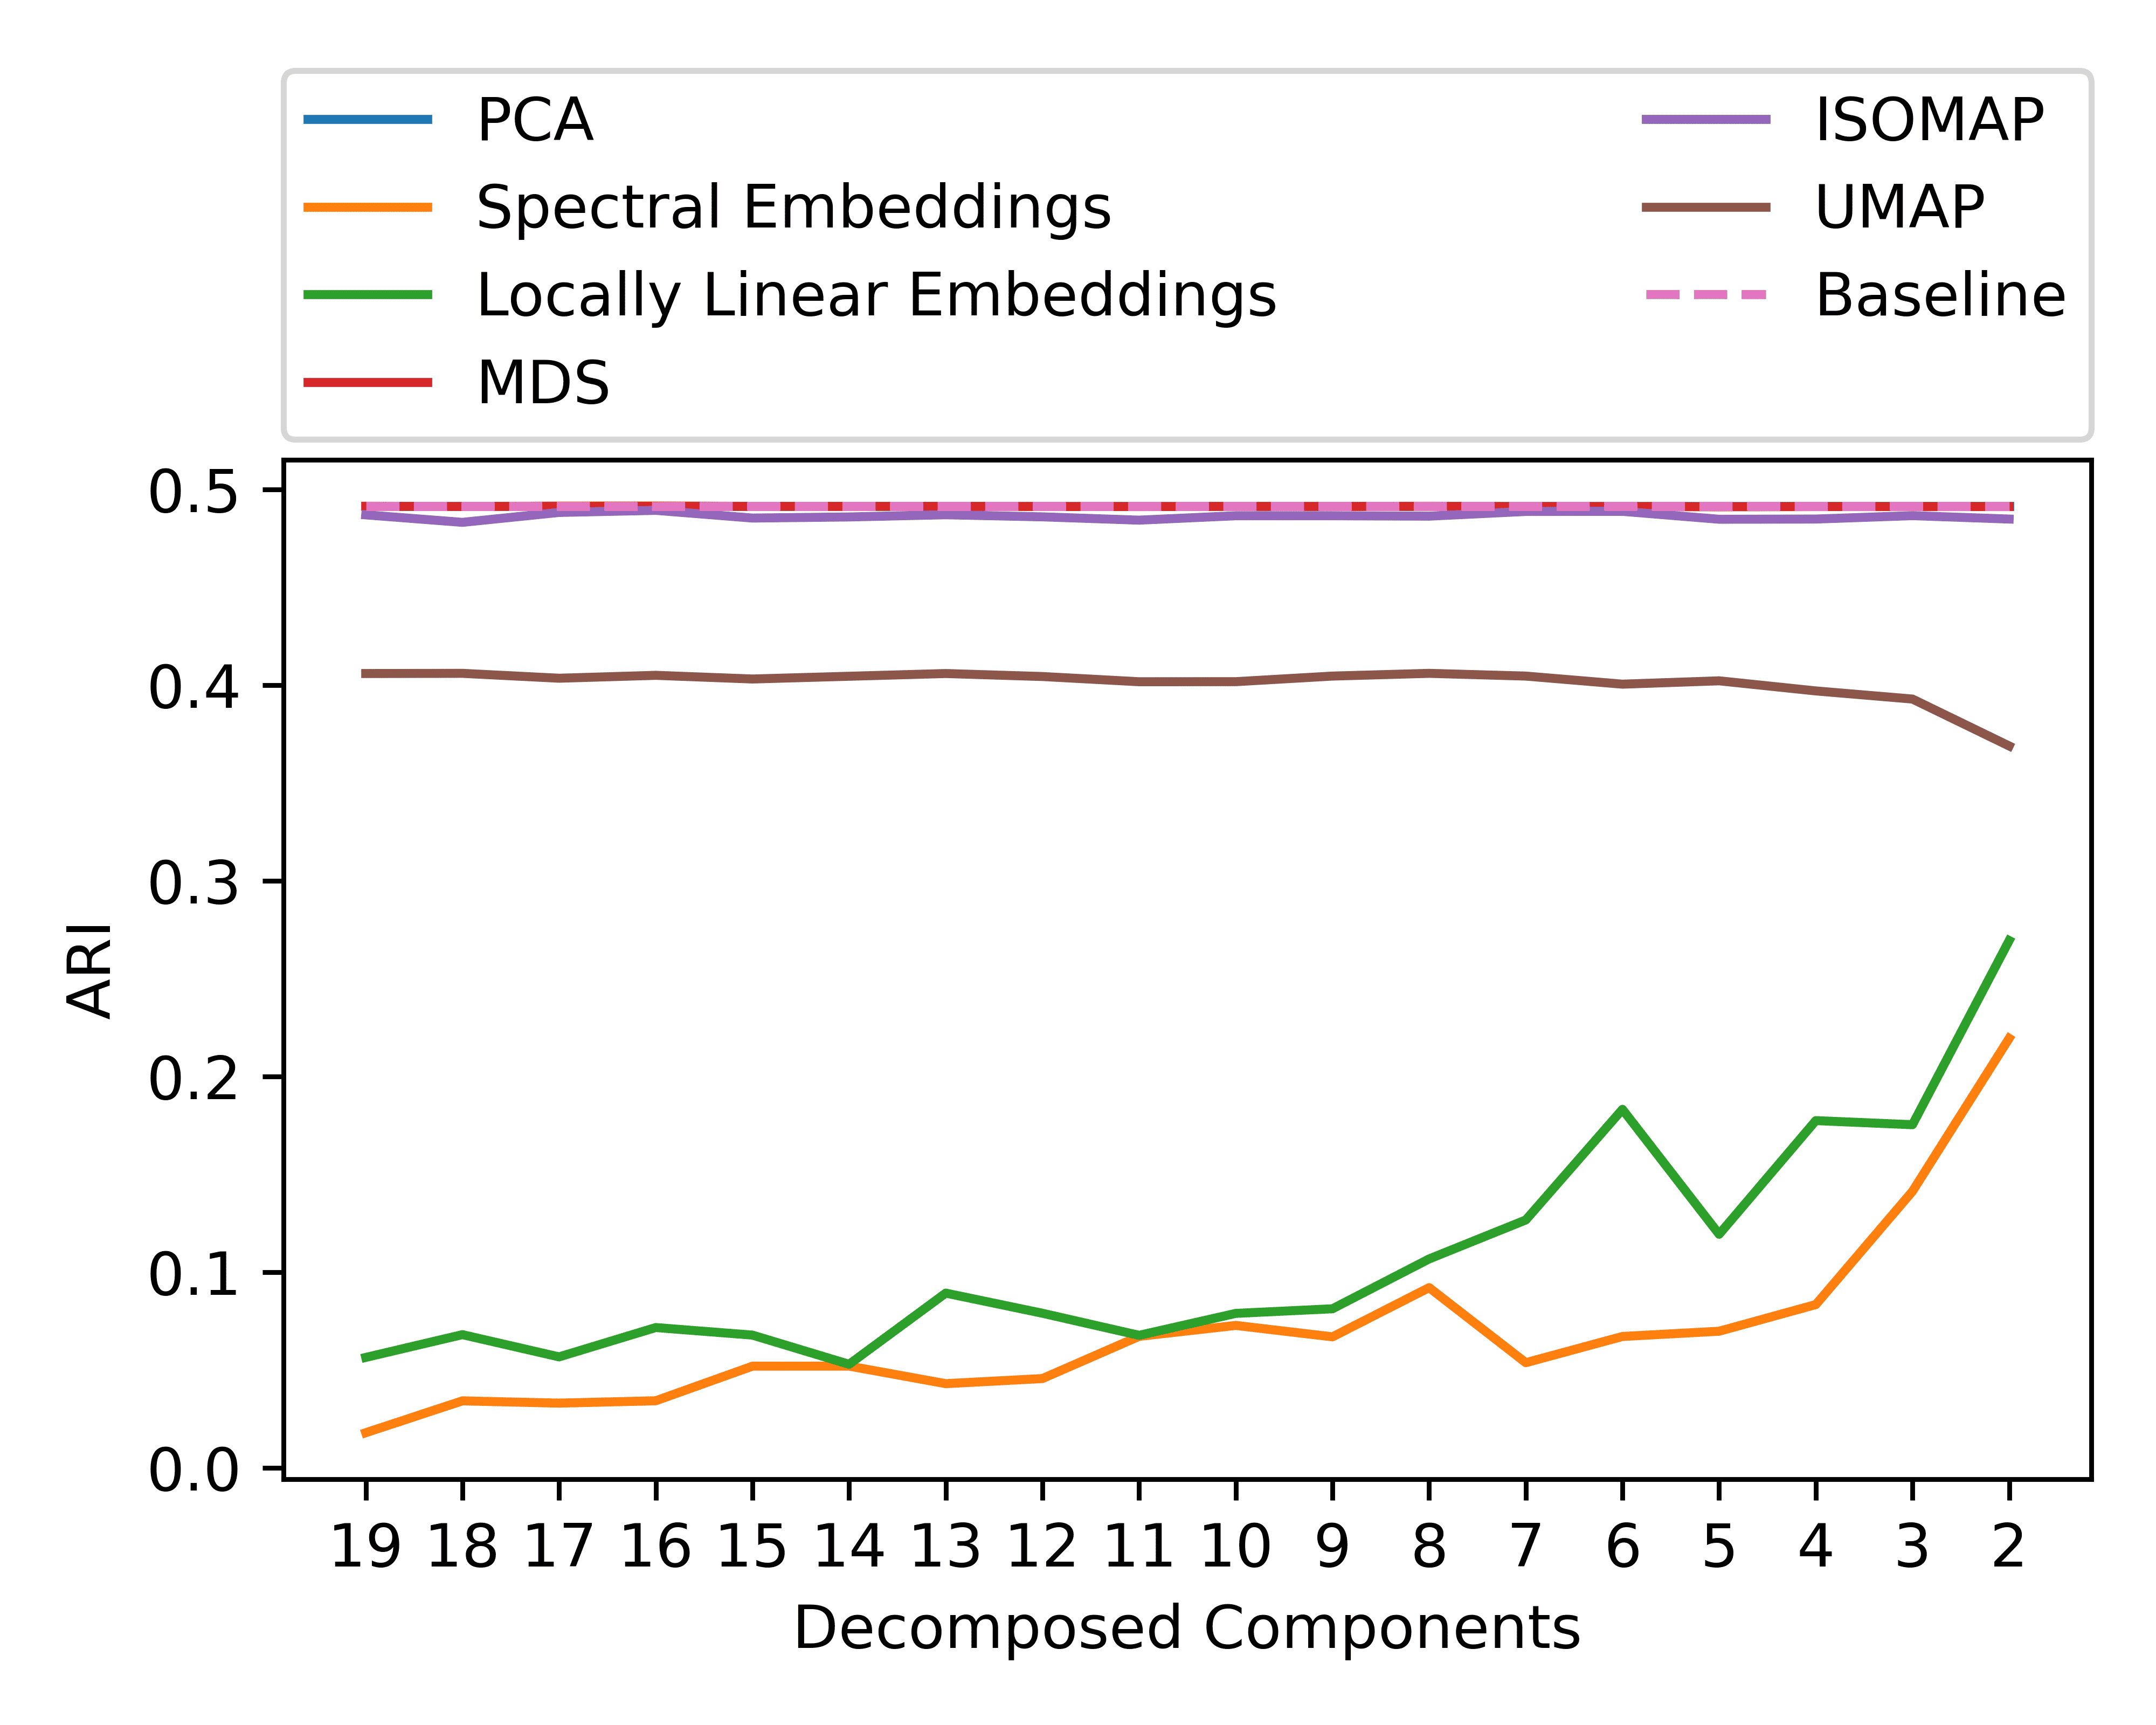
\includegraphics[width=0.48\linewidth]{images/charts_real/real_data_breast_cancer_ari.png}
                    \label{subfig:breast_cancer:ari}
                }
                \subfigure[]{
                    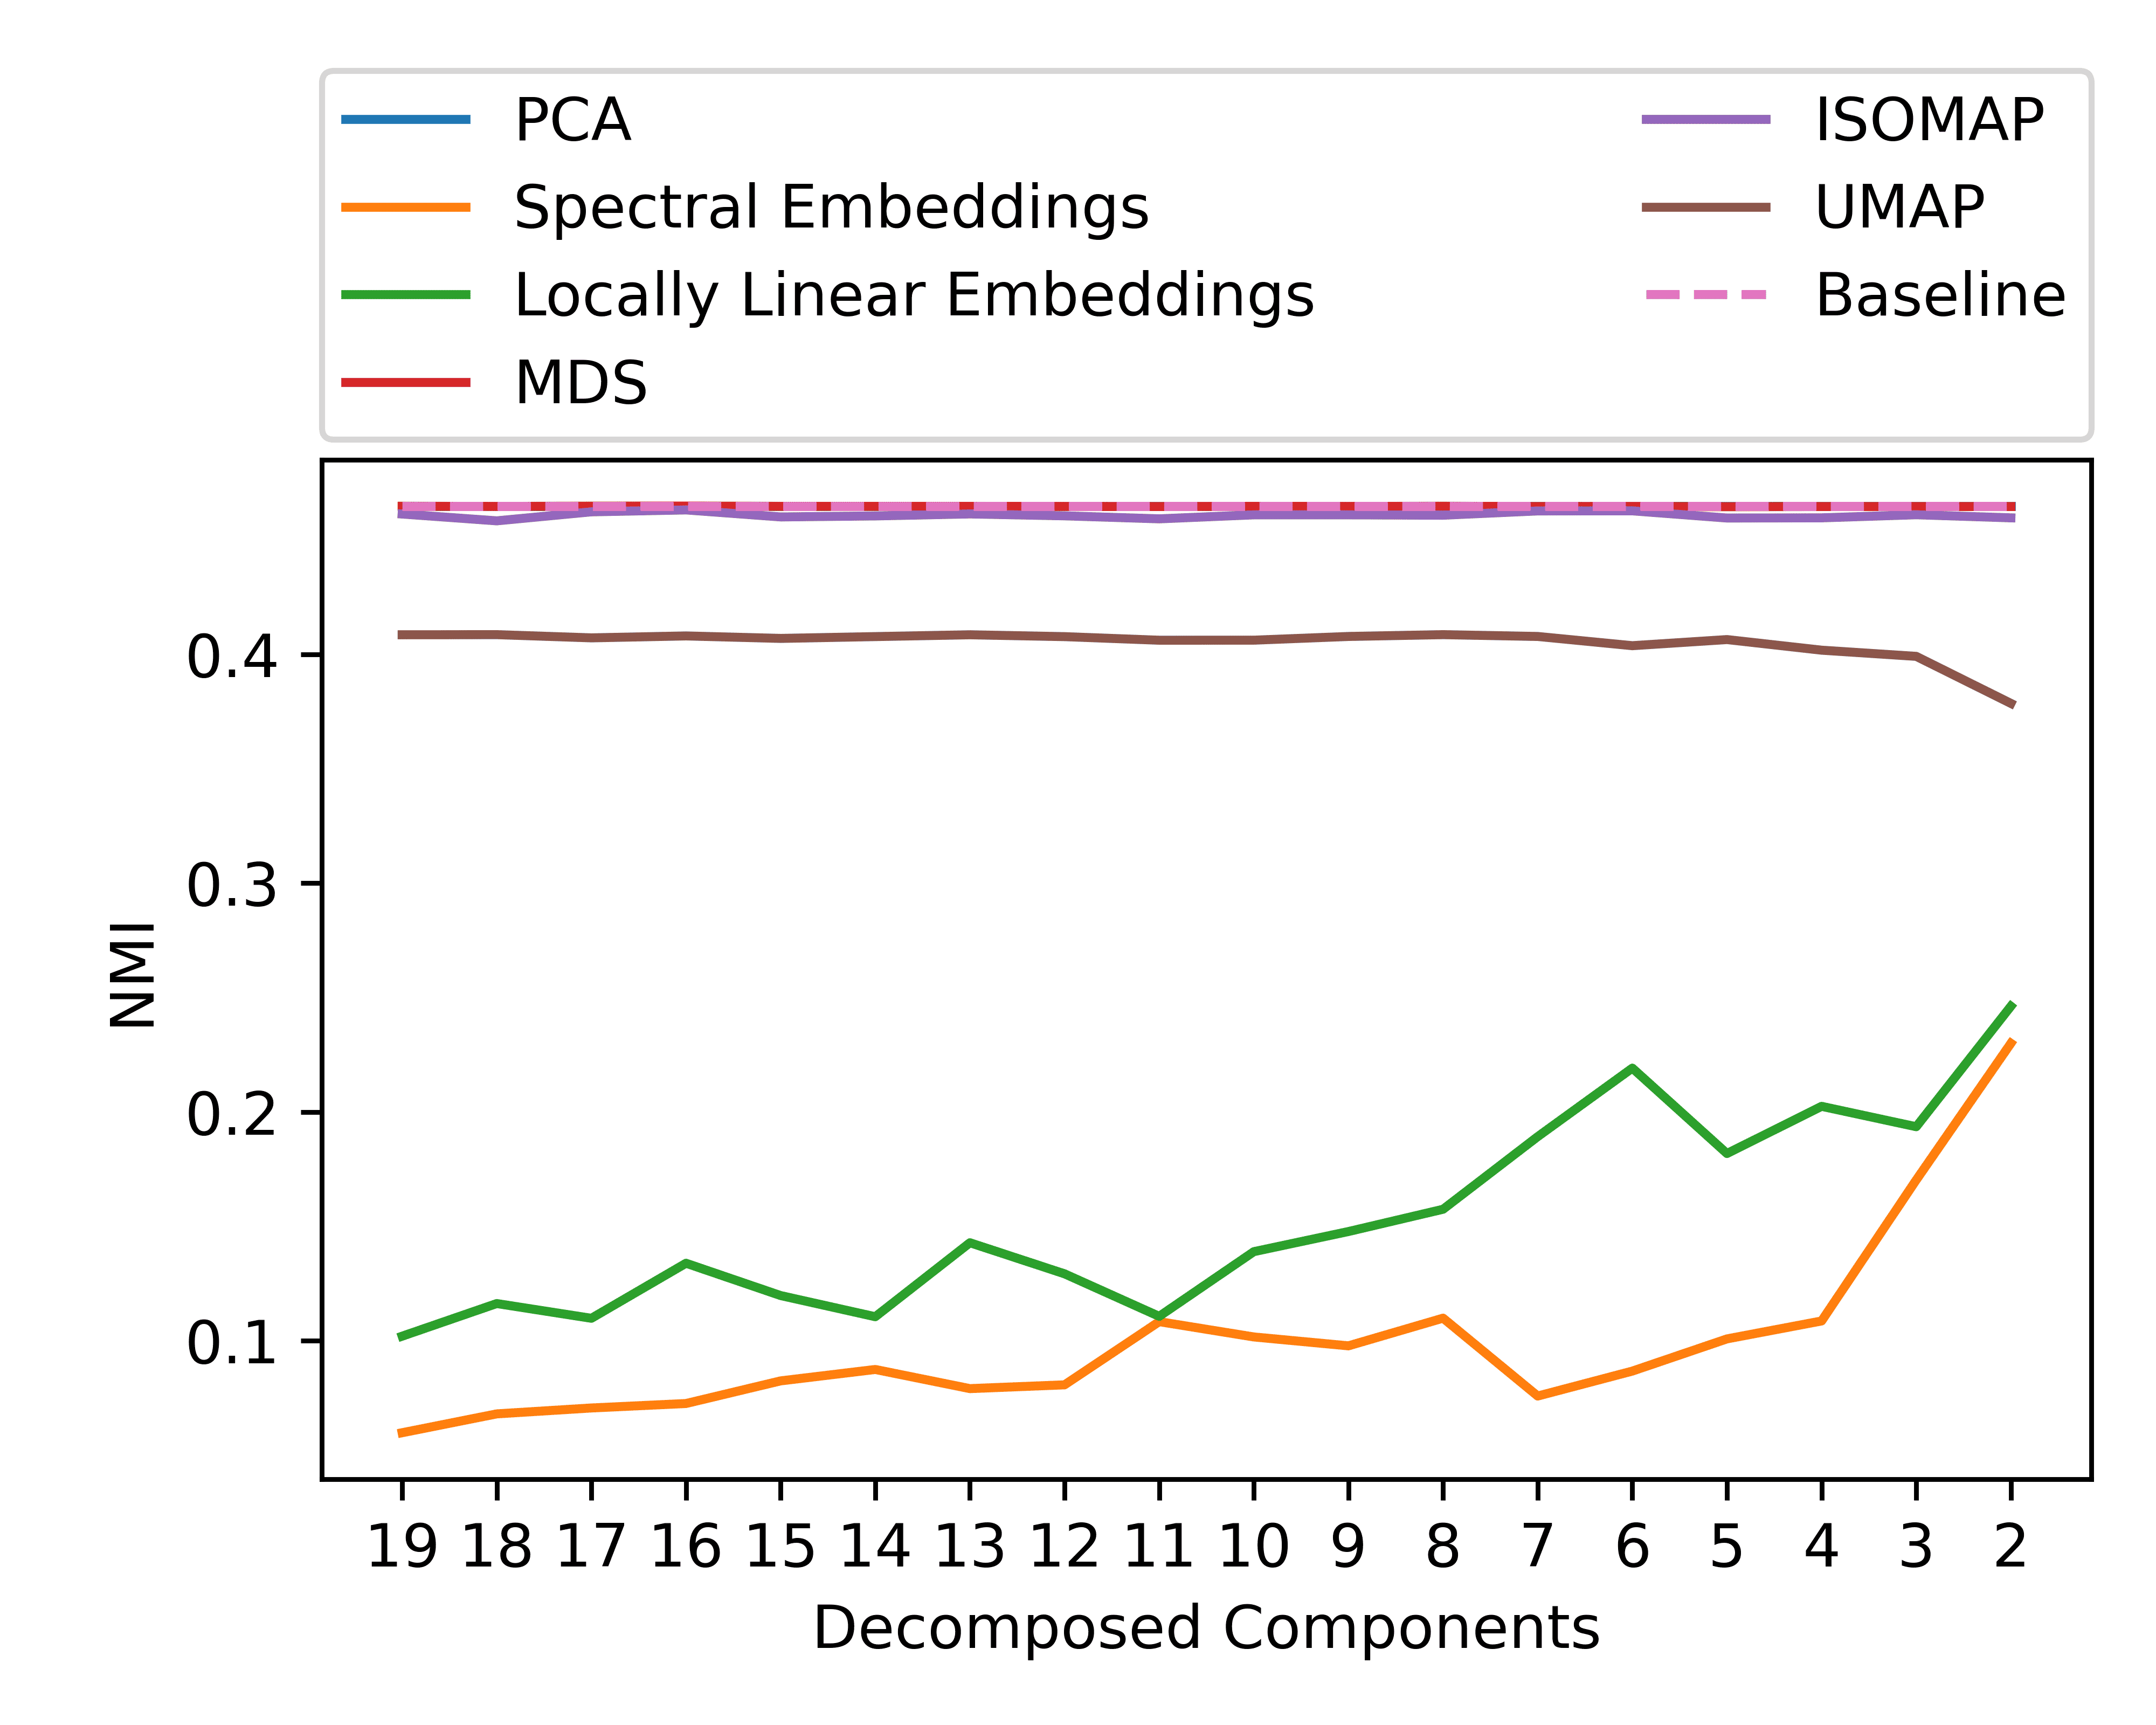
\includegraphics[width=0.48\linewidth]{images/charts_real/real_data_breast_cancer_nmi.png}
                    \label{subfig:breast_cancer:nmi}
                }
                \subfigure[]{
                    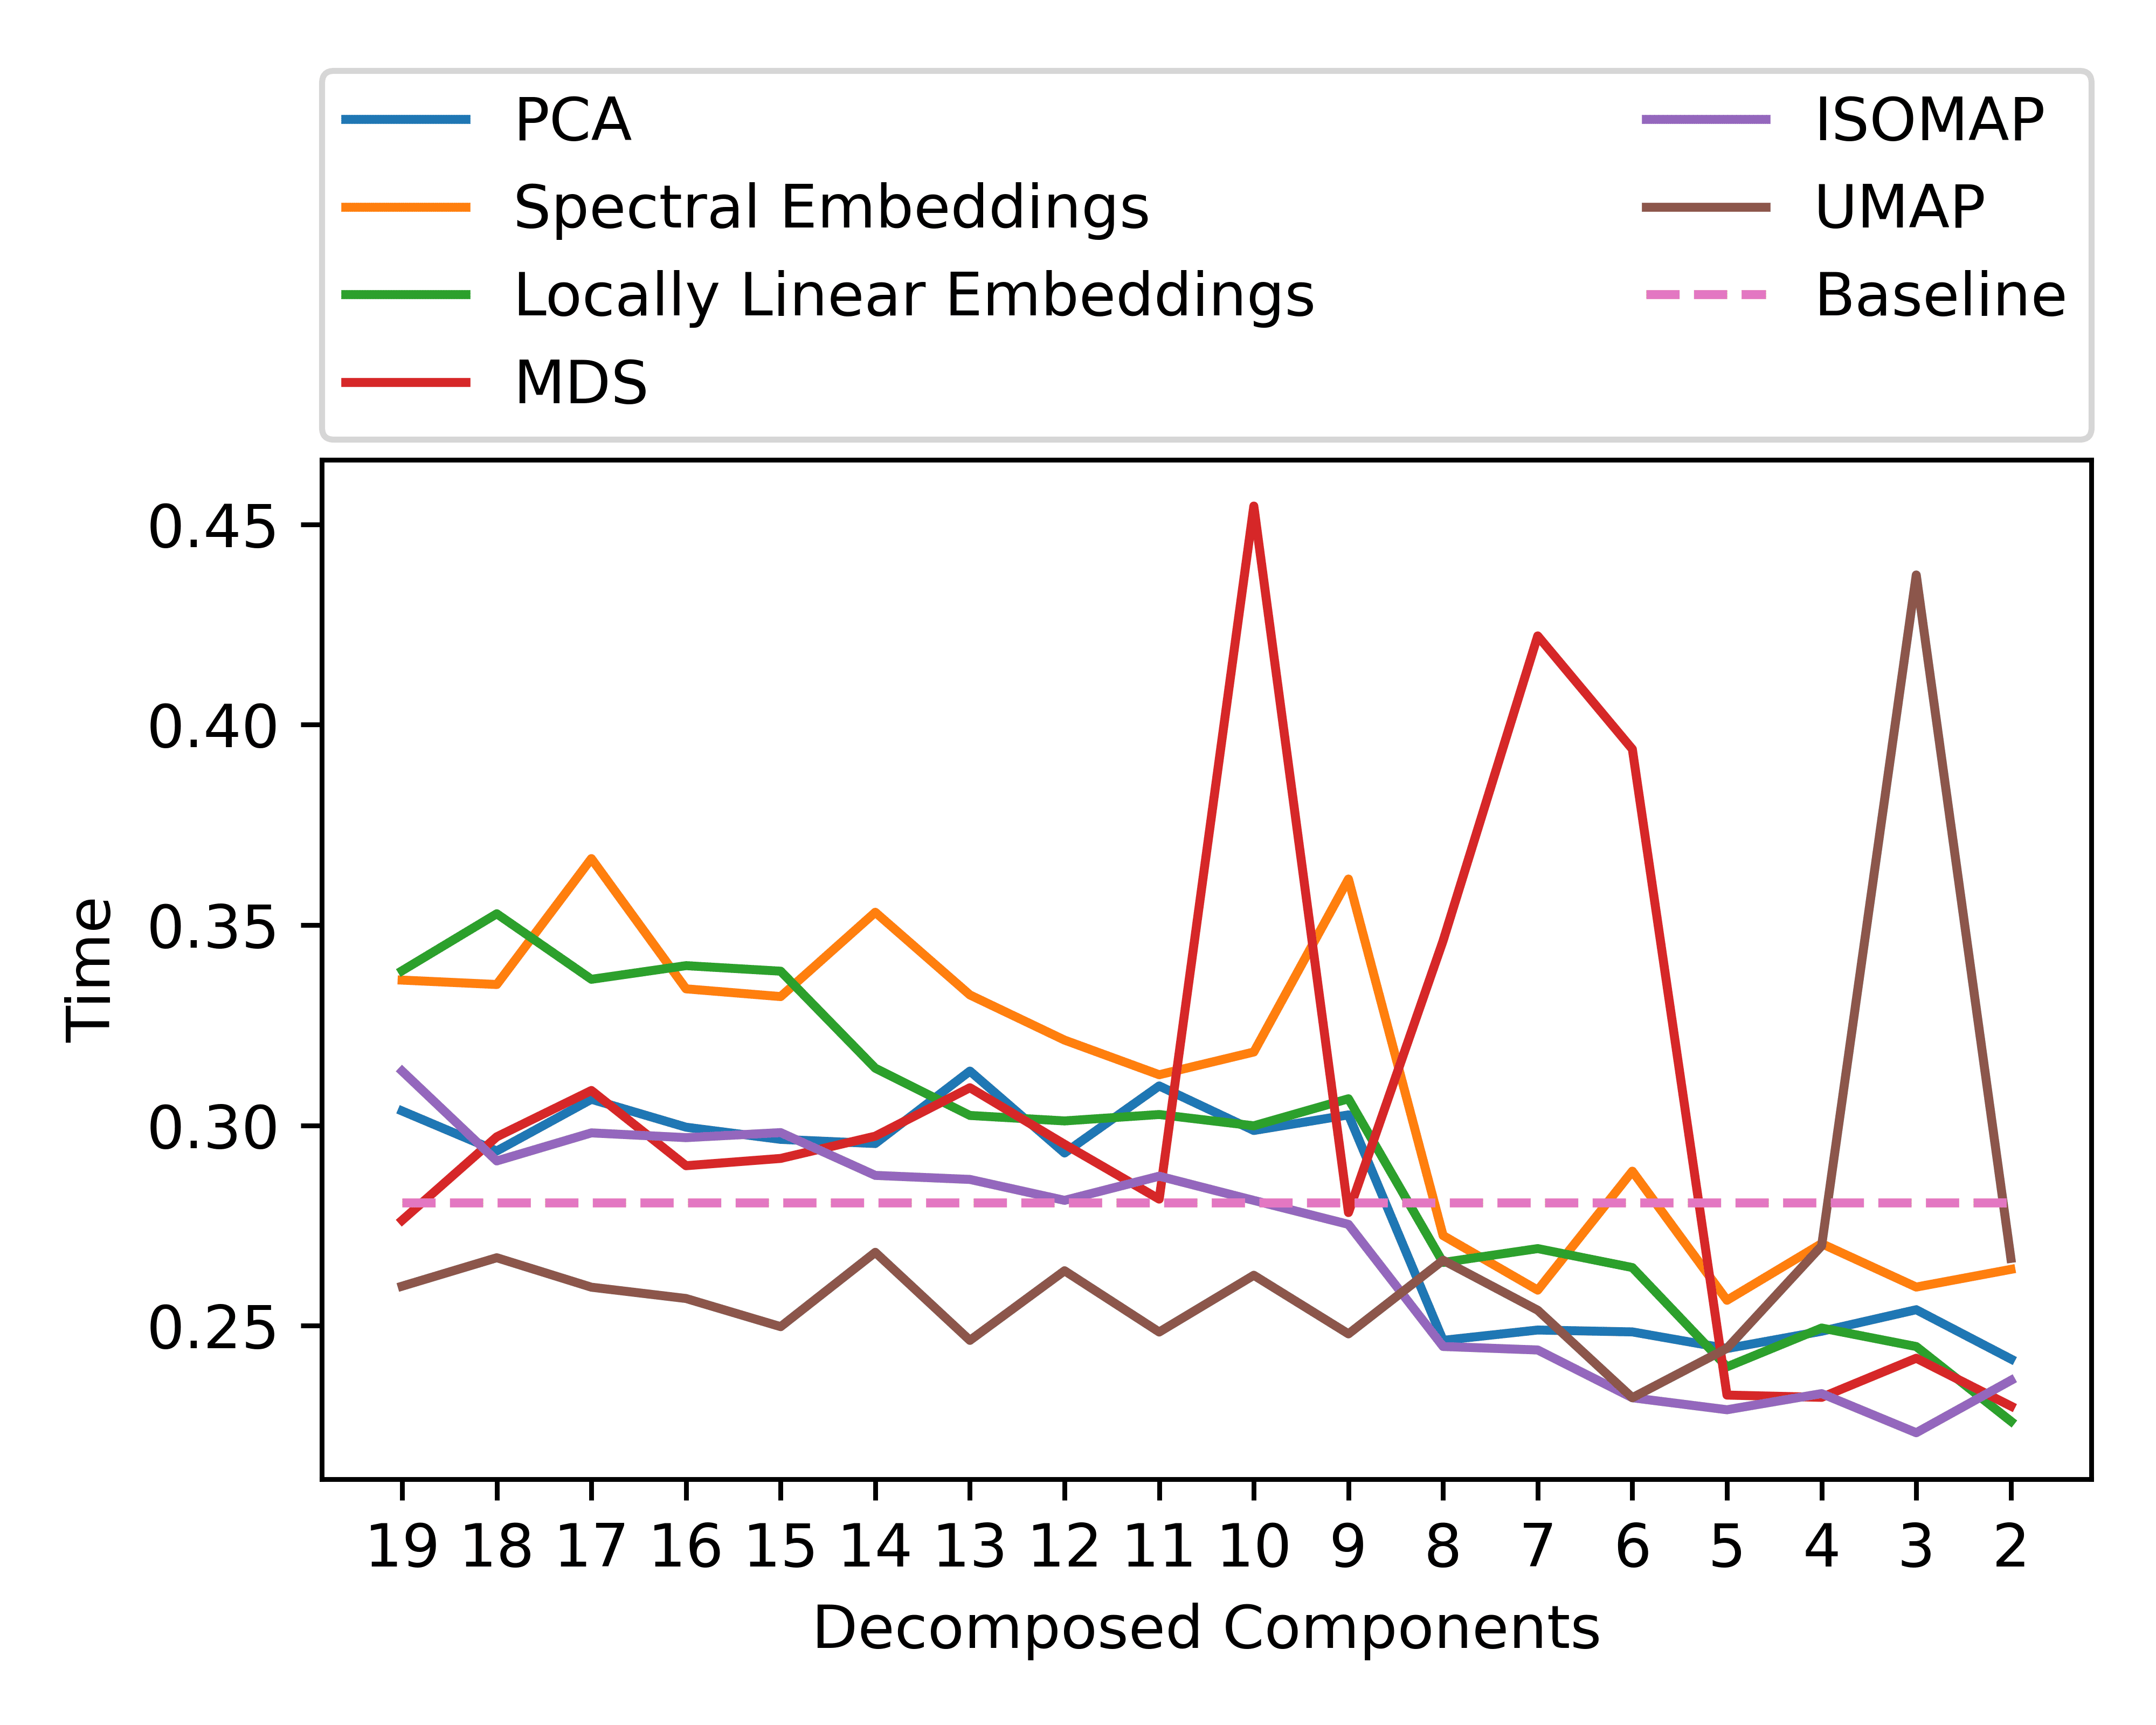
\includegraphics[width=0.48\linewidth]{images/charts_real/real_data_breast_cancer_time.png}
                    \label{subfig:breast_cancer:time}
                }
                \caption{Анализ влияния различных методов снижения размерности данных на кластеризацию набора данных Breast Cancer. Линия Baseline -- результат работы алгоритма \kmeans{} без предварительного снижения размерности. Результаты для
                    \subref{subfig:breast_cancer:ami} AMI;
                    \subref{subfig:breast_cancer:ari} ARI;
                    \subref{subfig:breast_cancer:nmi} NMI, а также на время работы алгоритма \subref{subfig:breast_cancer:time}.
                }
                \label{fig:breast_cancer}
            \end{figure}

            \begin{figure}[H]\centering
                \includegraphics[width=0.99\linewidth]{images/decomposer/breast_cancer_decomposer_analysis.png}
                \caption{Визуализация набора данных Breast Cancer после снижения размерности до 2 с использованием PCA, Spectral Embeddings, Locally Linear Embeddings, MDS, ISOMAP, UMAP.}
                \label{fig:breast_cancer:example}
            \end{figure}

            На рисунке \ref{fig:breast_cancer} представлены результаты применения различных методов снижения размерности перед кластеризацией K-Means на наборе данных Breast Cancer. Наиболее заметную положительную динамику продемонстрировали методы Locally Linear Embeddings (LLE) и Spectral Embeddings -- при уменьшении размерности до 10 и ниже наблюдается последовательный рост метрик кластеризации: AMI, ARI и NMI. Пиковые значения достигаются в точке, где число компонент совпадает с числом кластеров в выборке, что может свидетельствовать о более точной структурной декомпозиции, когда размерность пространства отражает истинное количество скрытых групп. В то же время алгоритмы PCA и MDS демонстрируют стабильные показатели качества, близкие к базовому сценарию кластеризации без предварительного снижения размерности. Это указывает на то, что оба метода хорошо сохраняют глобальную структуру данных, которая является ключевой для работы алгоритма K-Means. Особенно стоит отметить MDS, который обеспечивает не только стабильность качества, но и высокую воспроизводимость результатов на всем диапазоне размерностей. Такое поведение подтверждает различия в подходах: методы LLE и Spectral Embeddings склонны акцентировать внимание на локальных взаимосвязях между точками, что делает их полезными при сильной редукции, в то время как PCA и MDS сохраняют глобальную топологию, важную для более устойчивой кластеризации.

        \subsubsection{Результаты алгоритма на наборе данных Digits}
            Digits -- это стандартный набор данных для многоклассовой классификации, часто используемый в задачах распознавания образов. Данные представляют собой рукописные цифры от 0 до 9, оцифрованные в виде изображений 8x8 пикселей. Каждое изображение преобразовано в матрицу чисел, отражающих интенсивность оттенков серого.

            \begin{table}[H]
                \centering
                \caption{Характеристики набора данных Digits.}
                \begin{tabular}{ccc}
                    \toprule
                    Число классов & Число объектов & Размерность пространства \\
                    \midrule
                    10 & 1797 & 64 \\
                    \bottomrule
                \end{tabular}
            \end{table}

            Набор данных Digits представляет собой матрицу размерностью 1797x64, где каждая строка соответствует одному изображению цифры, а каждый столбец содержит значение яркости пикселя (от 0 до 16). Исходные изображения были нормализованы для уменьшения влияния вариаций наклона и толщины линий.

            \begin{figure}[H]\centering
                \subfigure[]{
                    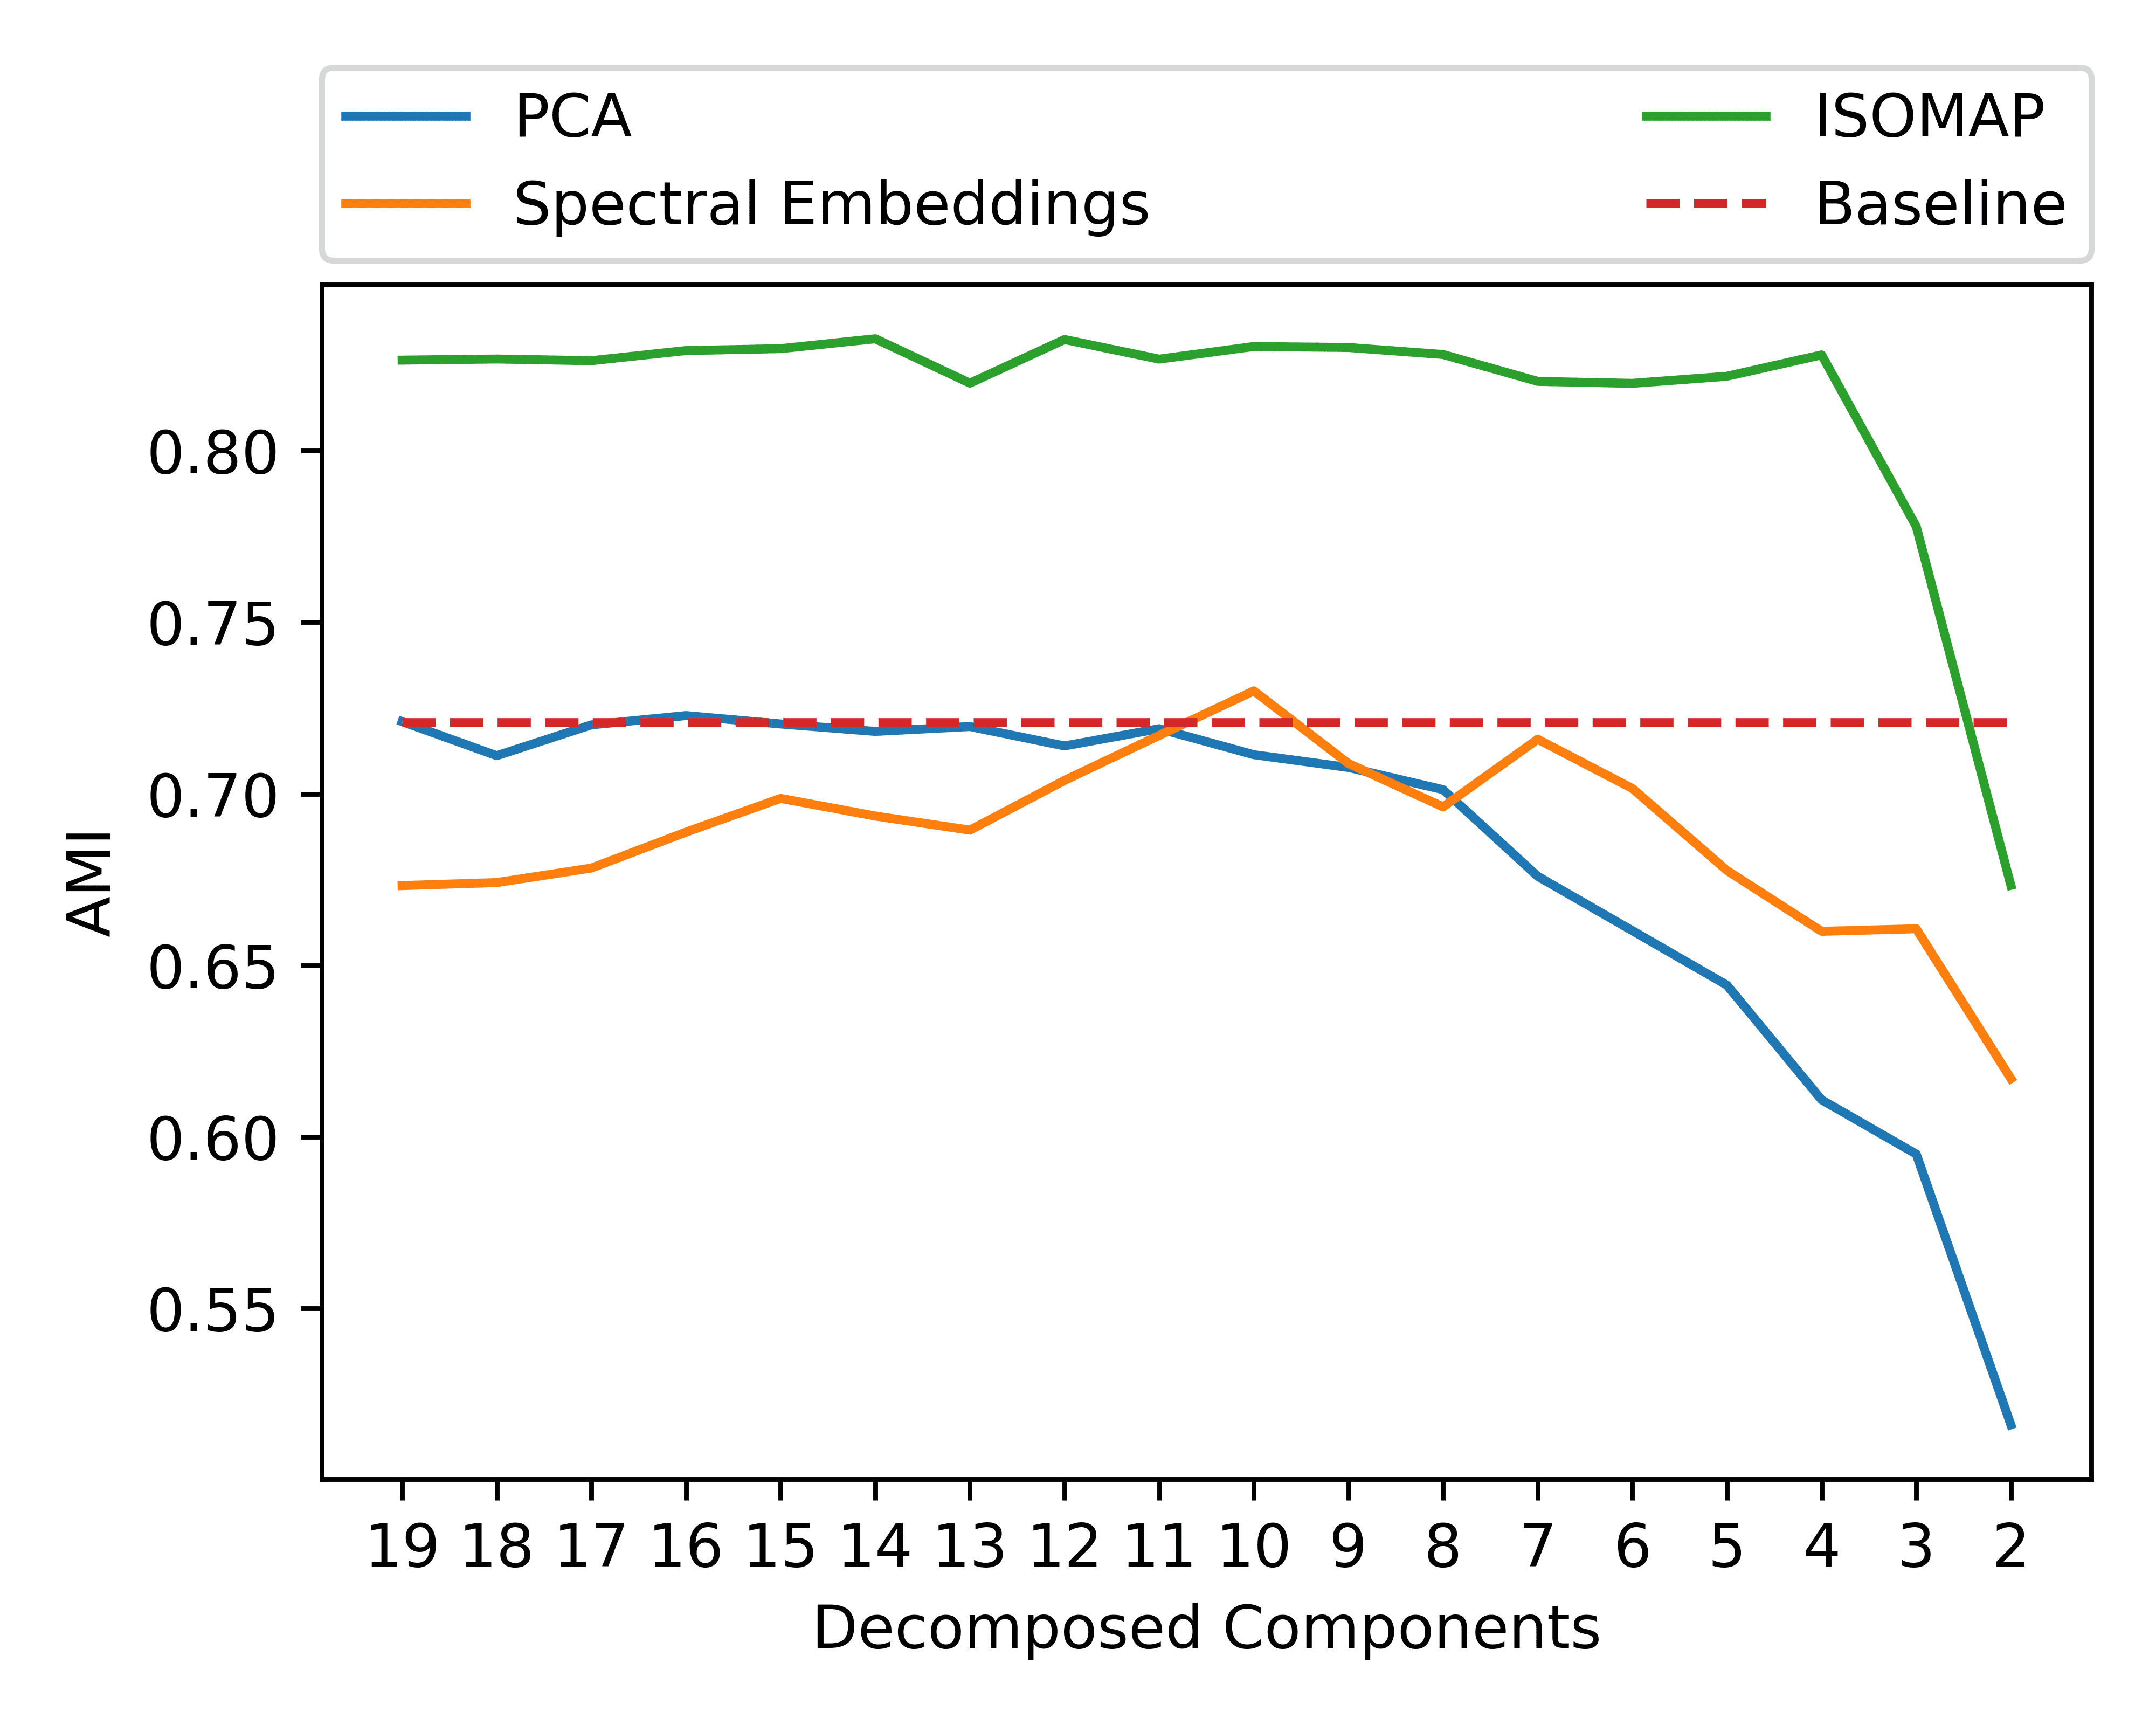
\includegraphics[width=0.48\linewidth]{images/charts_real/real_data_digits_ami.png}
                    \label{subfig:digits:ami}
                }
                \subfigure[]{
                    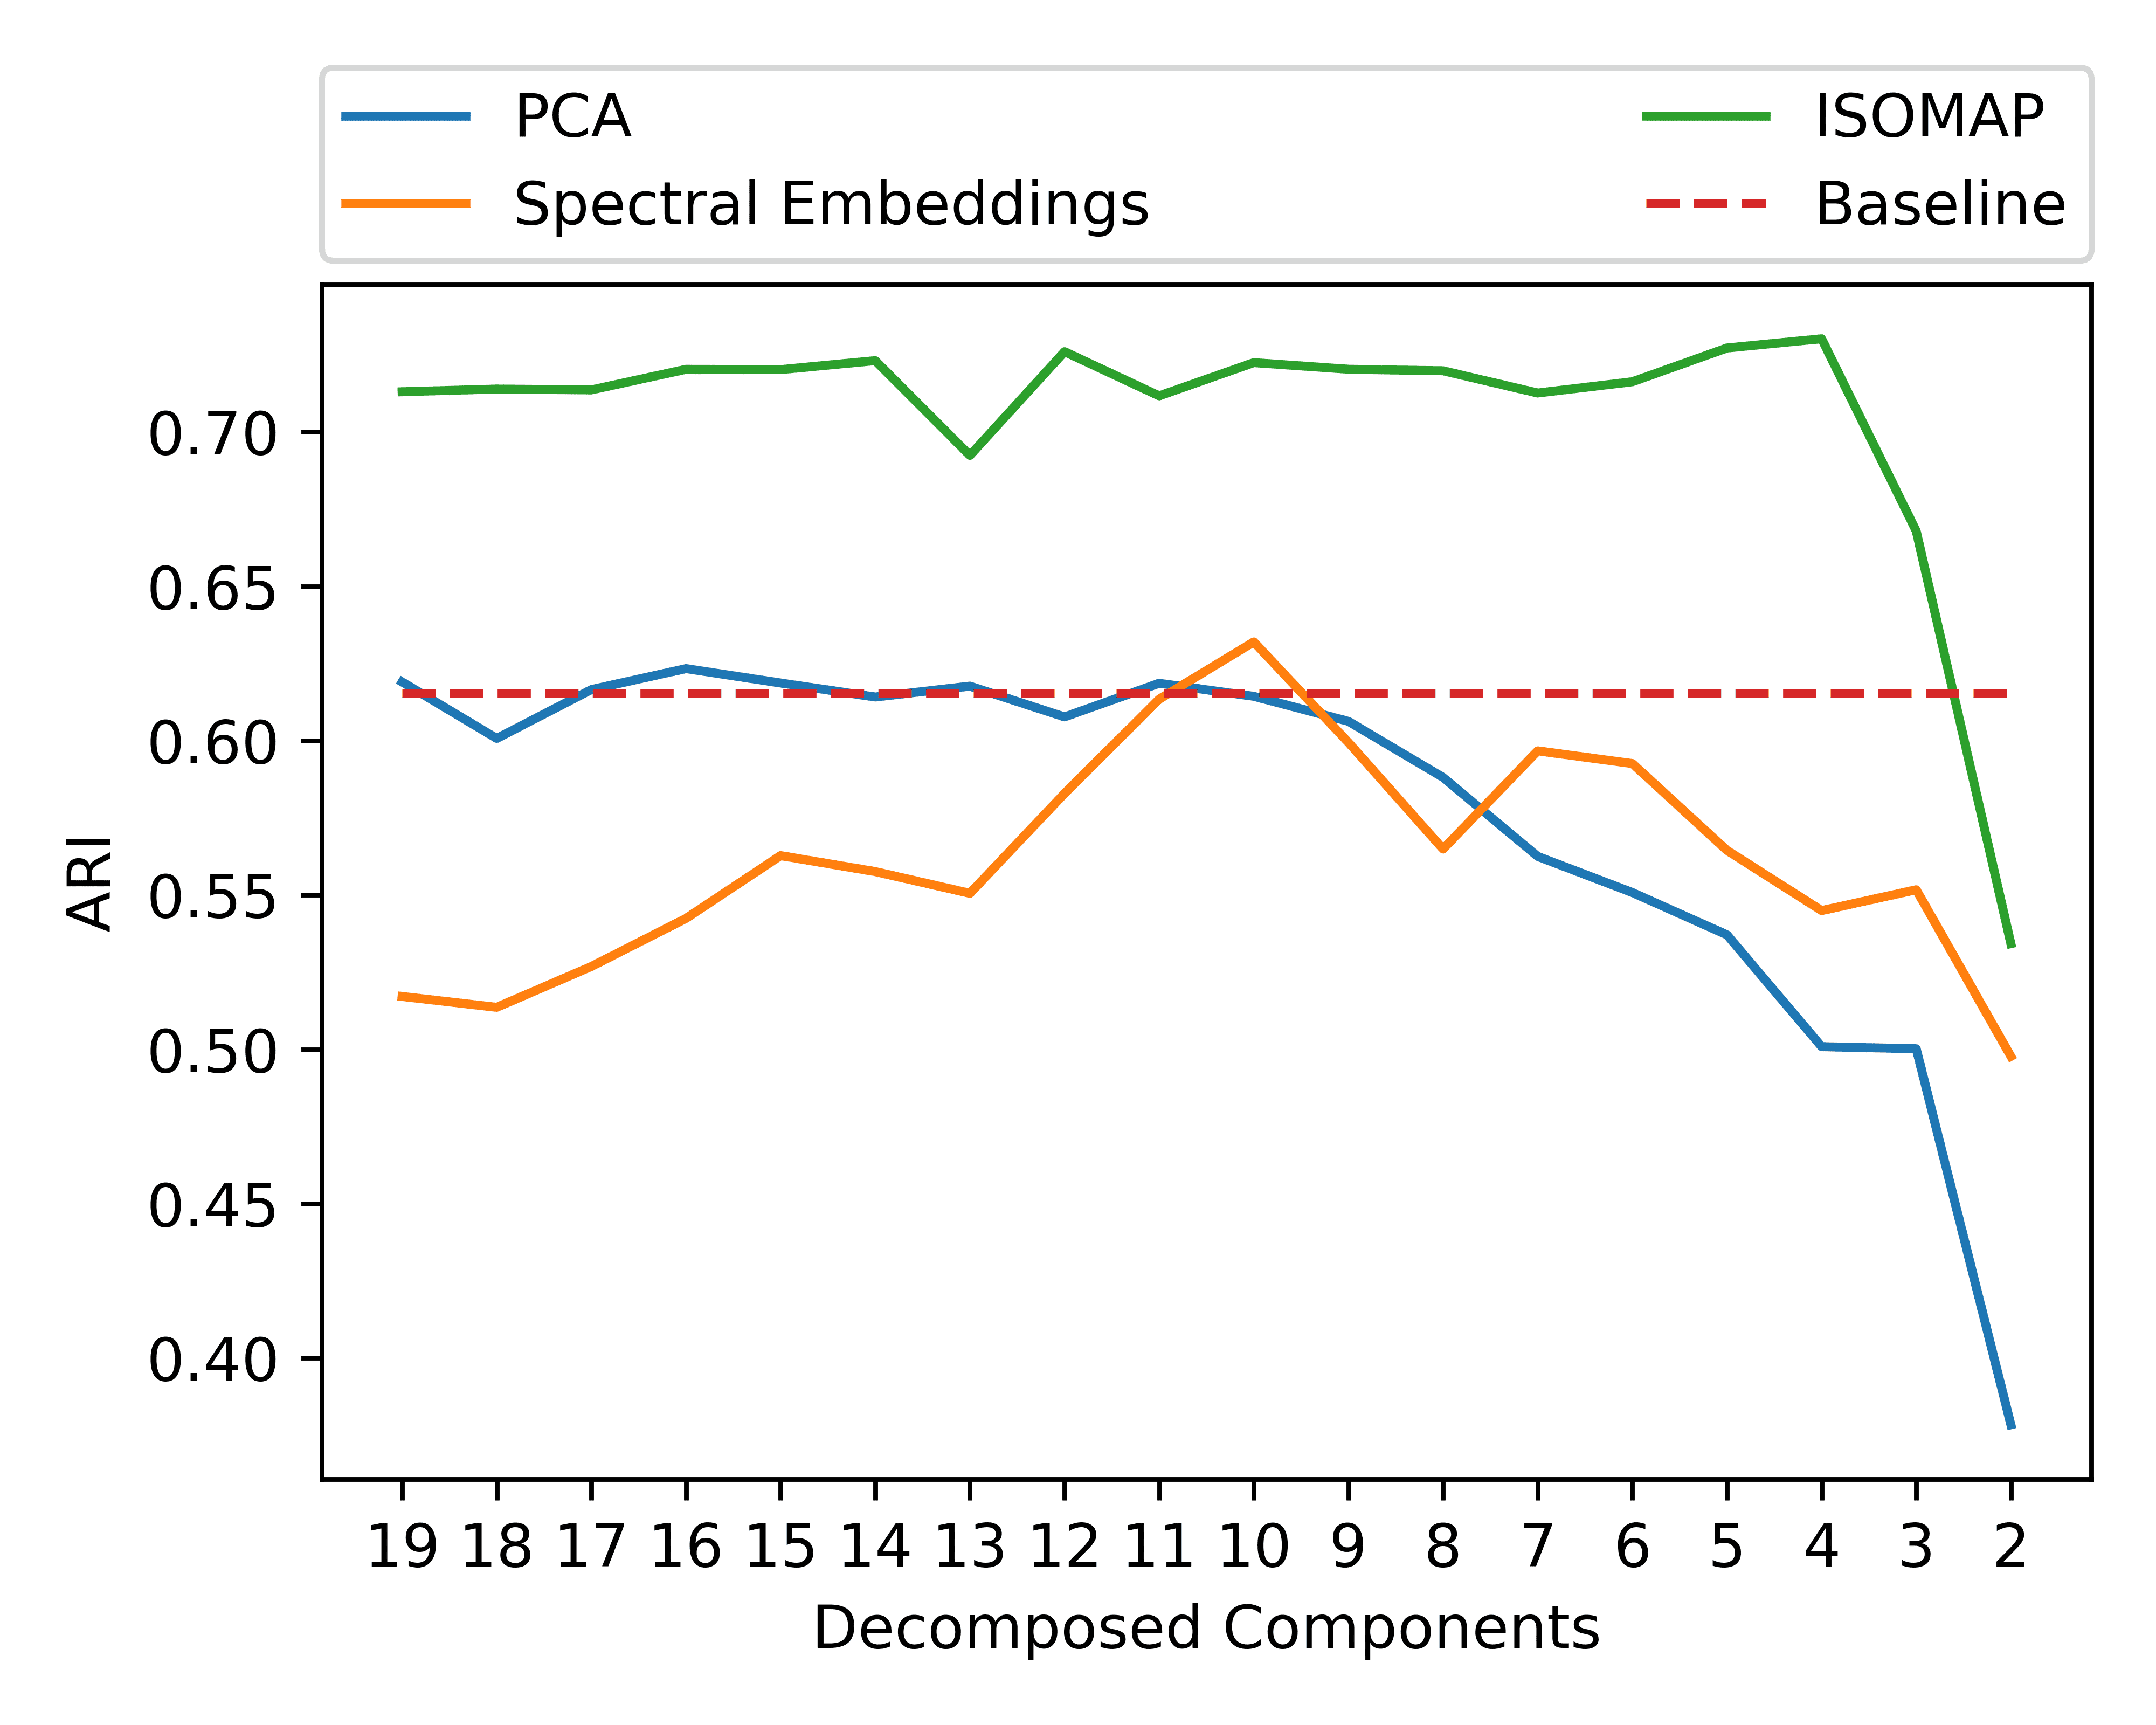
\includegraphics[width=0.48\linewidth]{images/charts_real/real_data_digits_ari.png}
                    \label{subfig:digits:ari}
                }
                \subfigure[]{
                    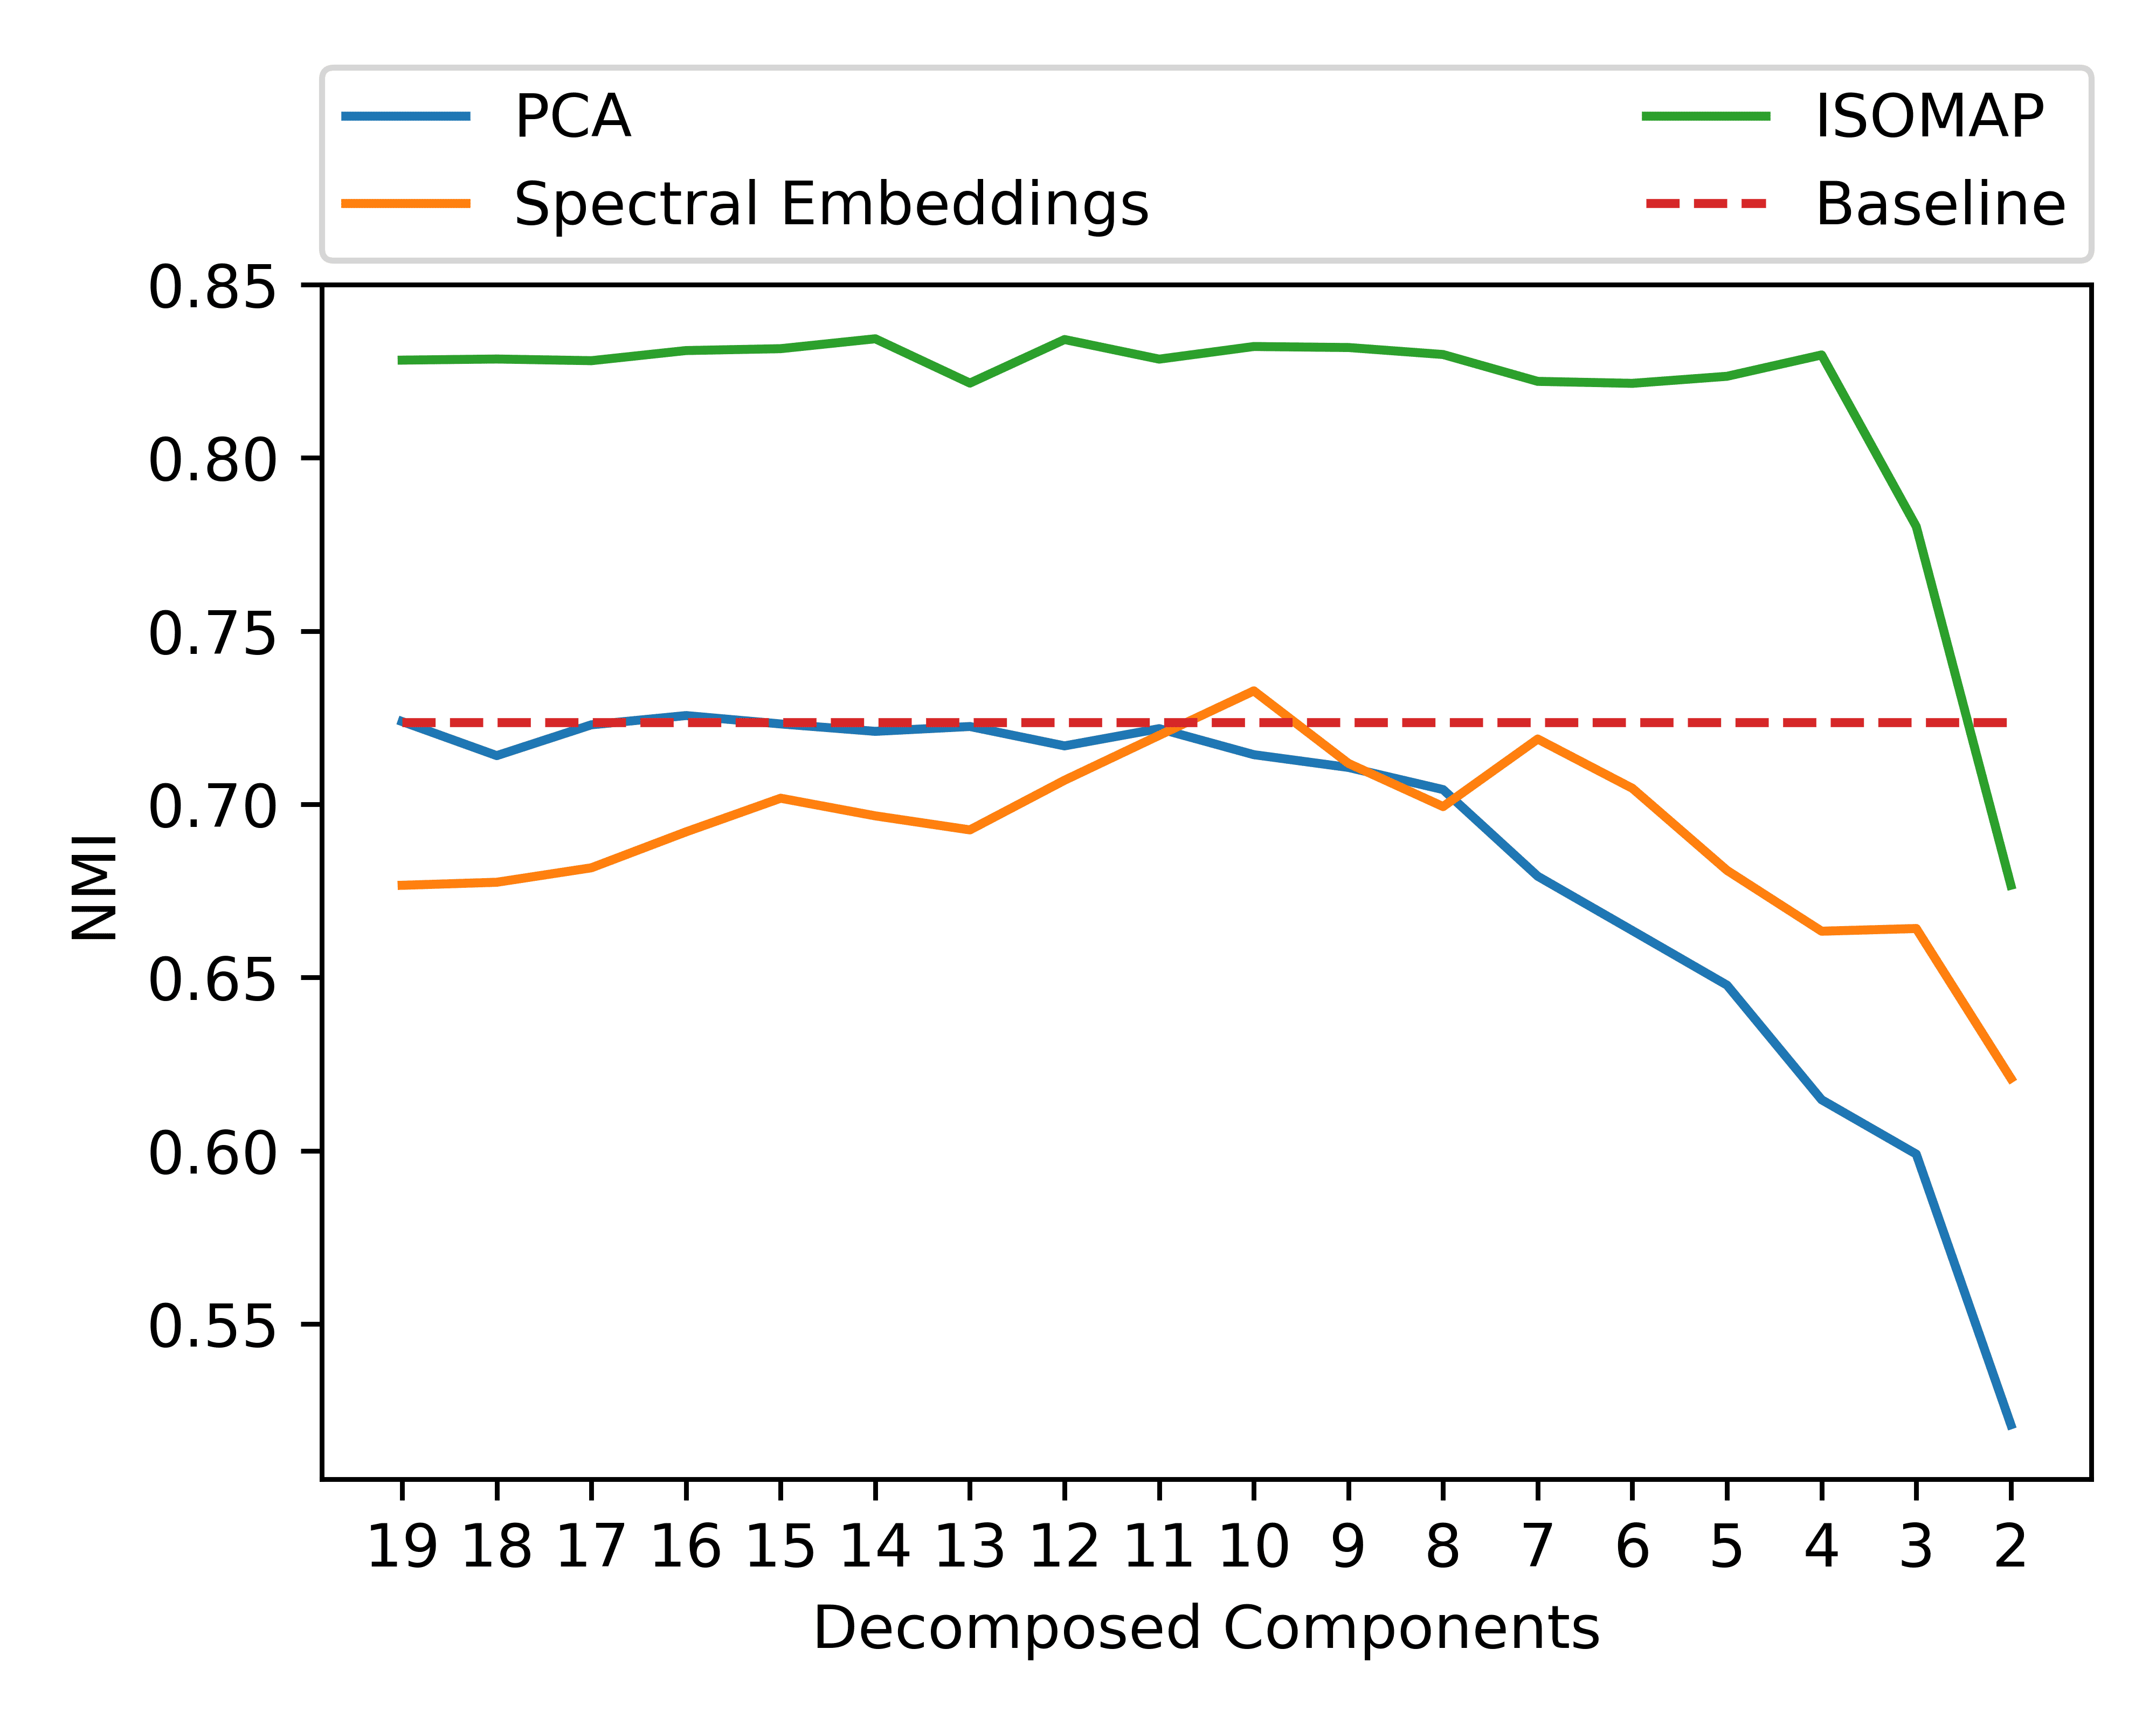
\includegraphics[width=0.48\linewidth]{images/charts_real/real_data_digits_nmi.png}
                    \label{subfig:digits:nmi}
                }
                \subfigure[]{
                    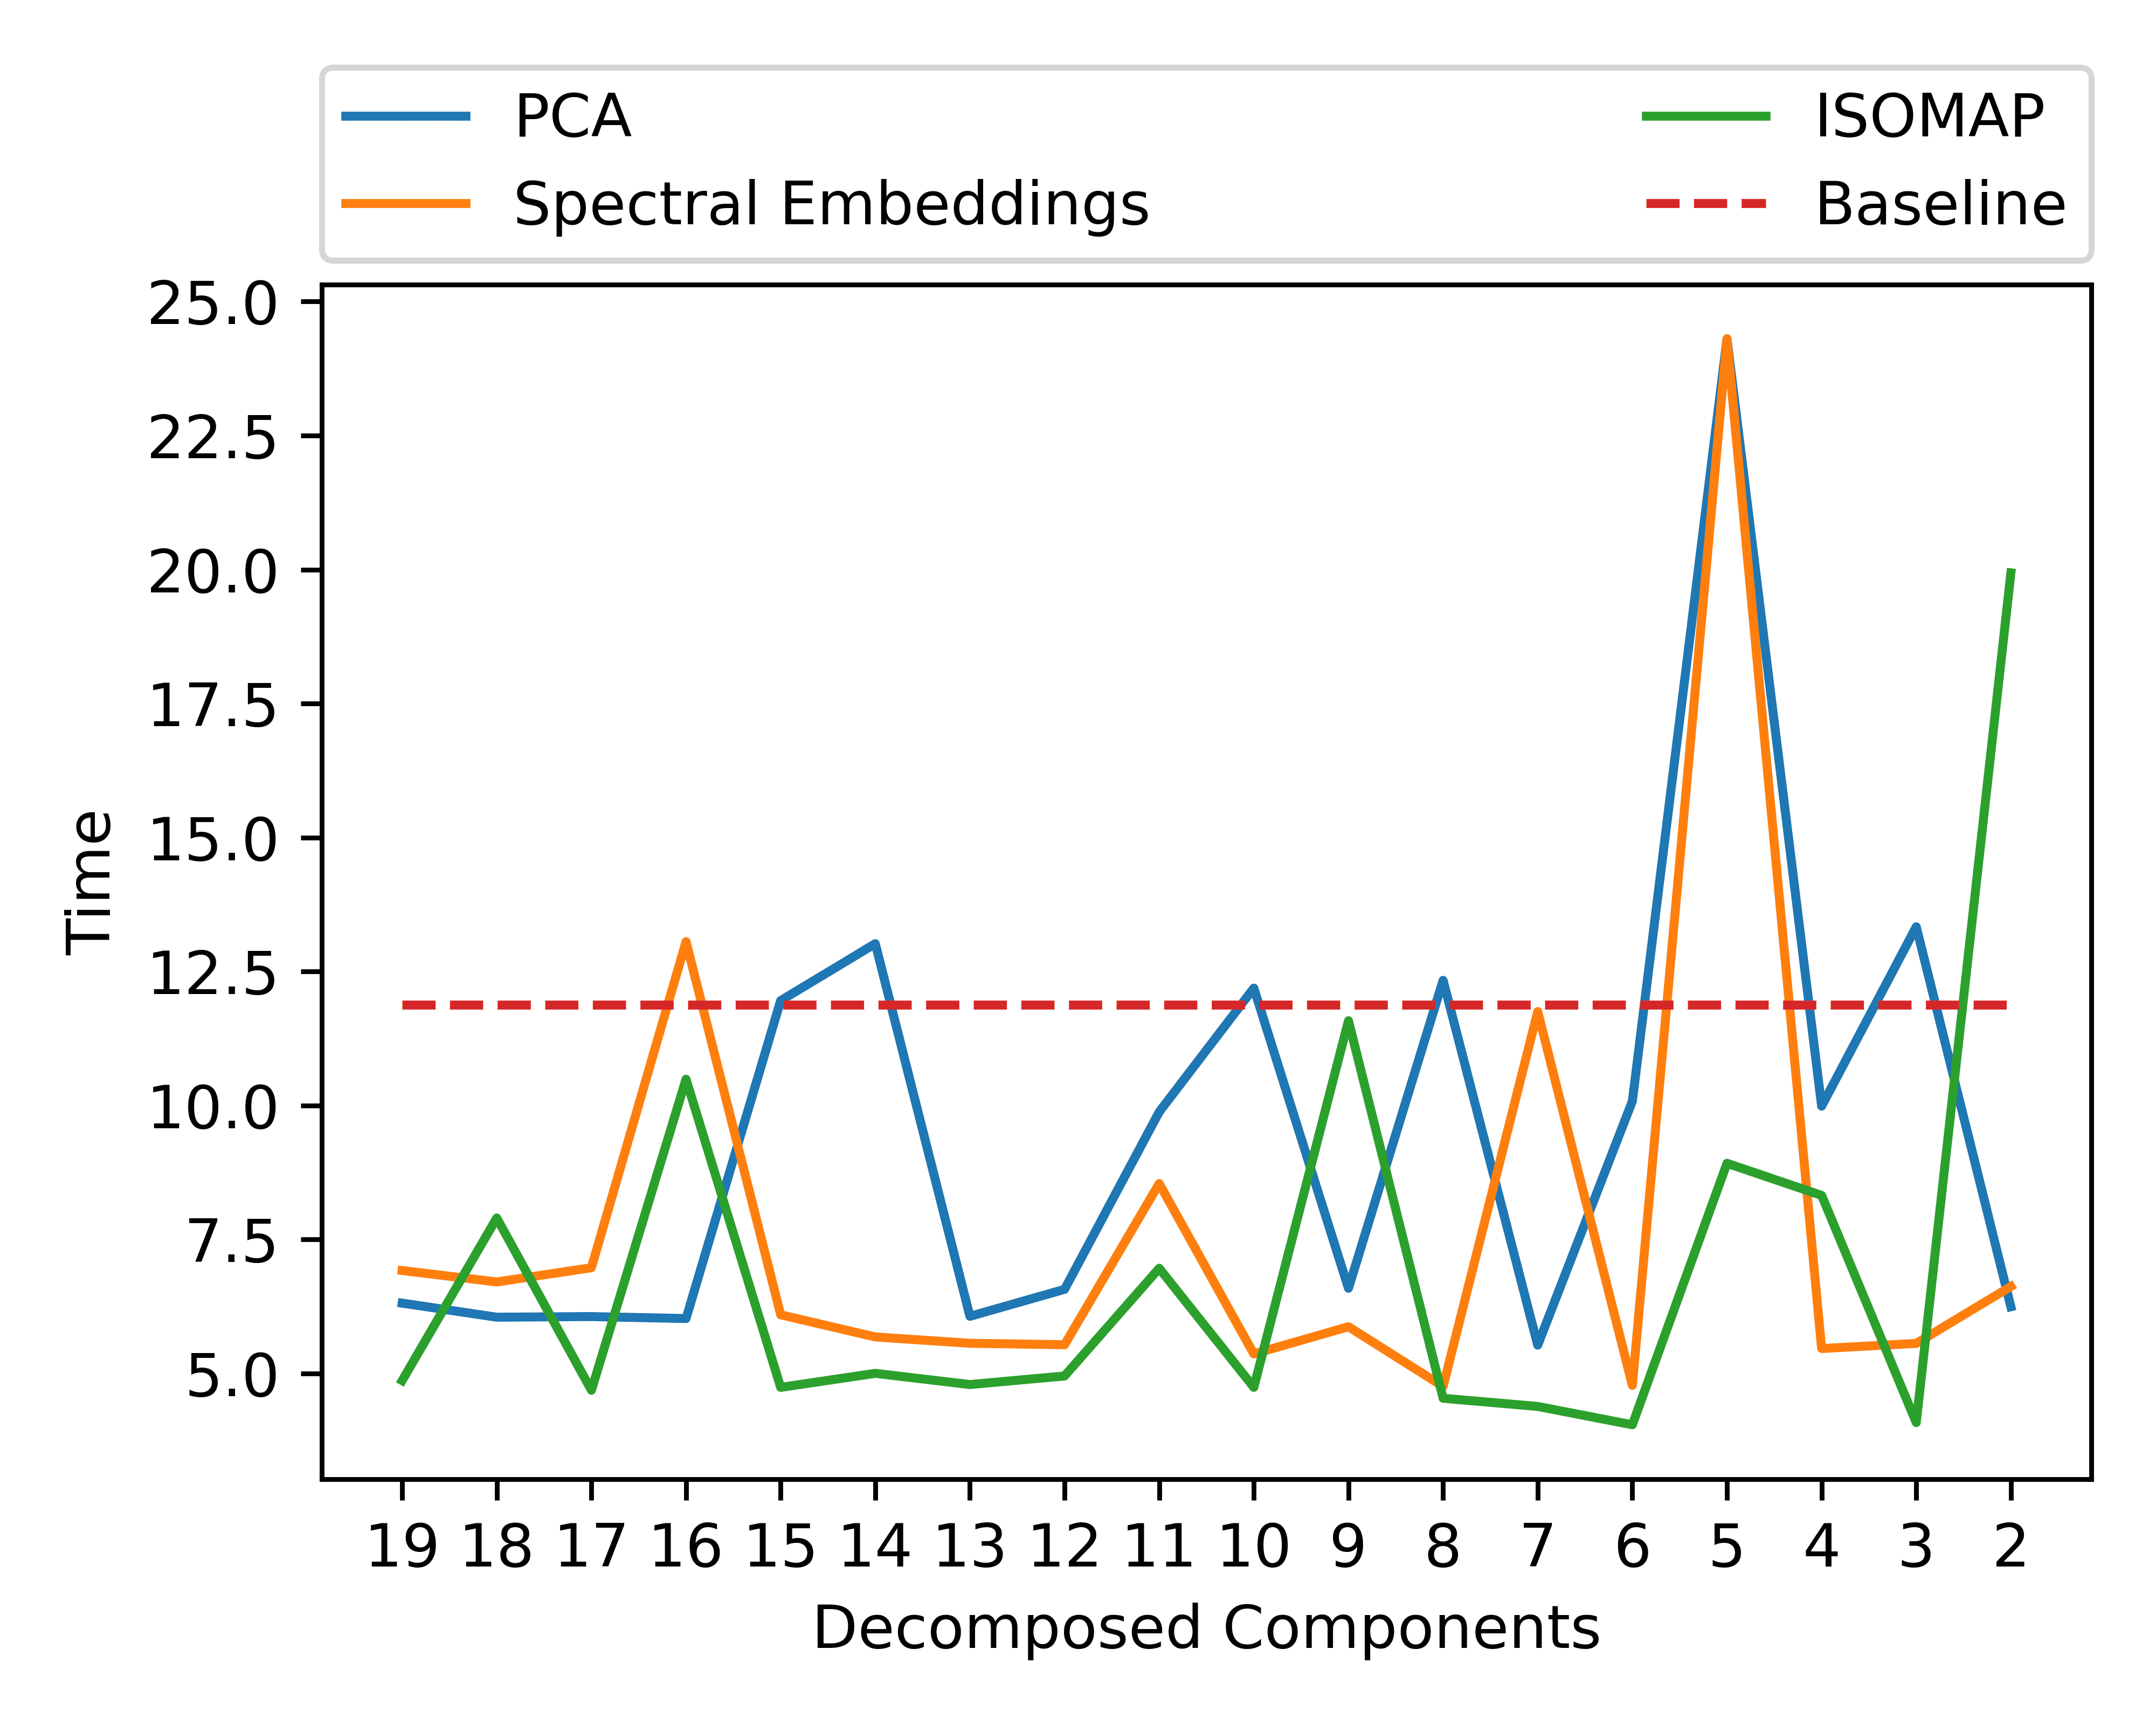
\includegraphics[width=0.48\linewidth]{images/charts_real/real_data_digits_time.png}
                    \label{subfig:digits:time}
                }
                \caption{Анализ влияния различных методов снижения размерности данных на кластеризацию набора данных Digits. Линия Baseline -- результат работы алгоритма \kmeans{} без предварительного снижения размерности. Результаты для
                    \subref{subfig:digits:ami} AMI;
                    \subref{subfig:digits:ari} ARI;
                    \subref{subfig:digits:nmi} NMI, а также на время работы алгоритма \subref{subfig:digits:time}.
                }
                \label{fig:digits}
            \end{figure}

            \begin{figure}[H]\centering
                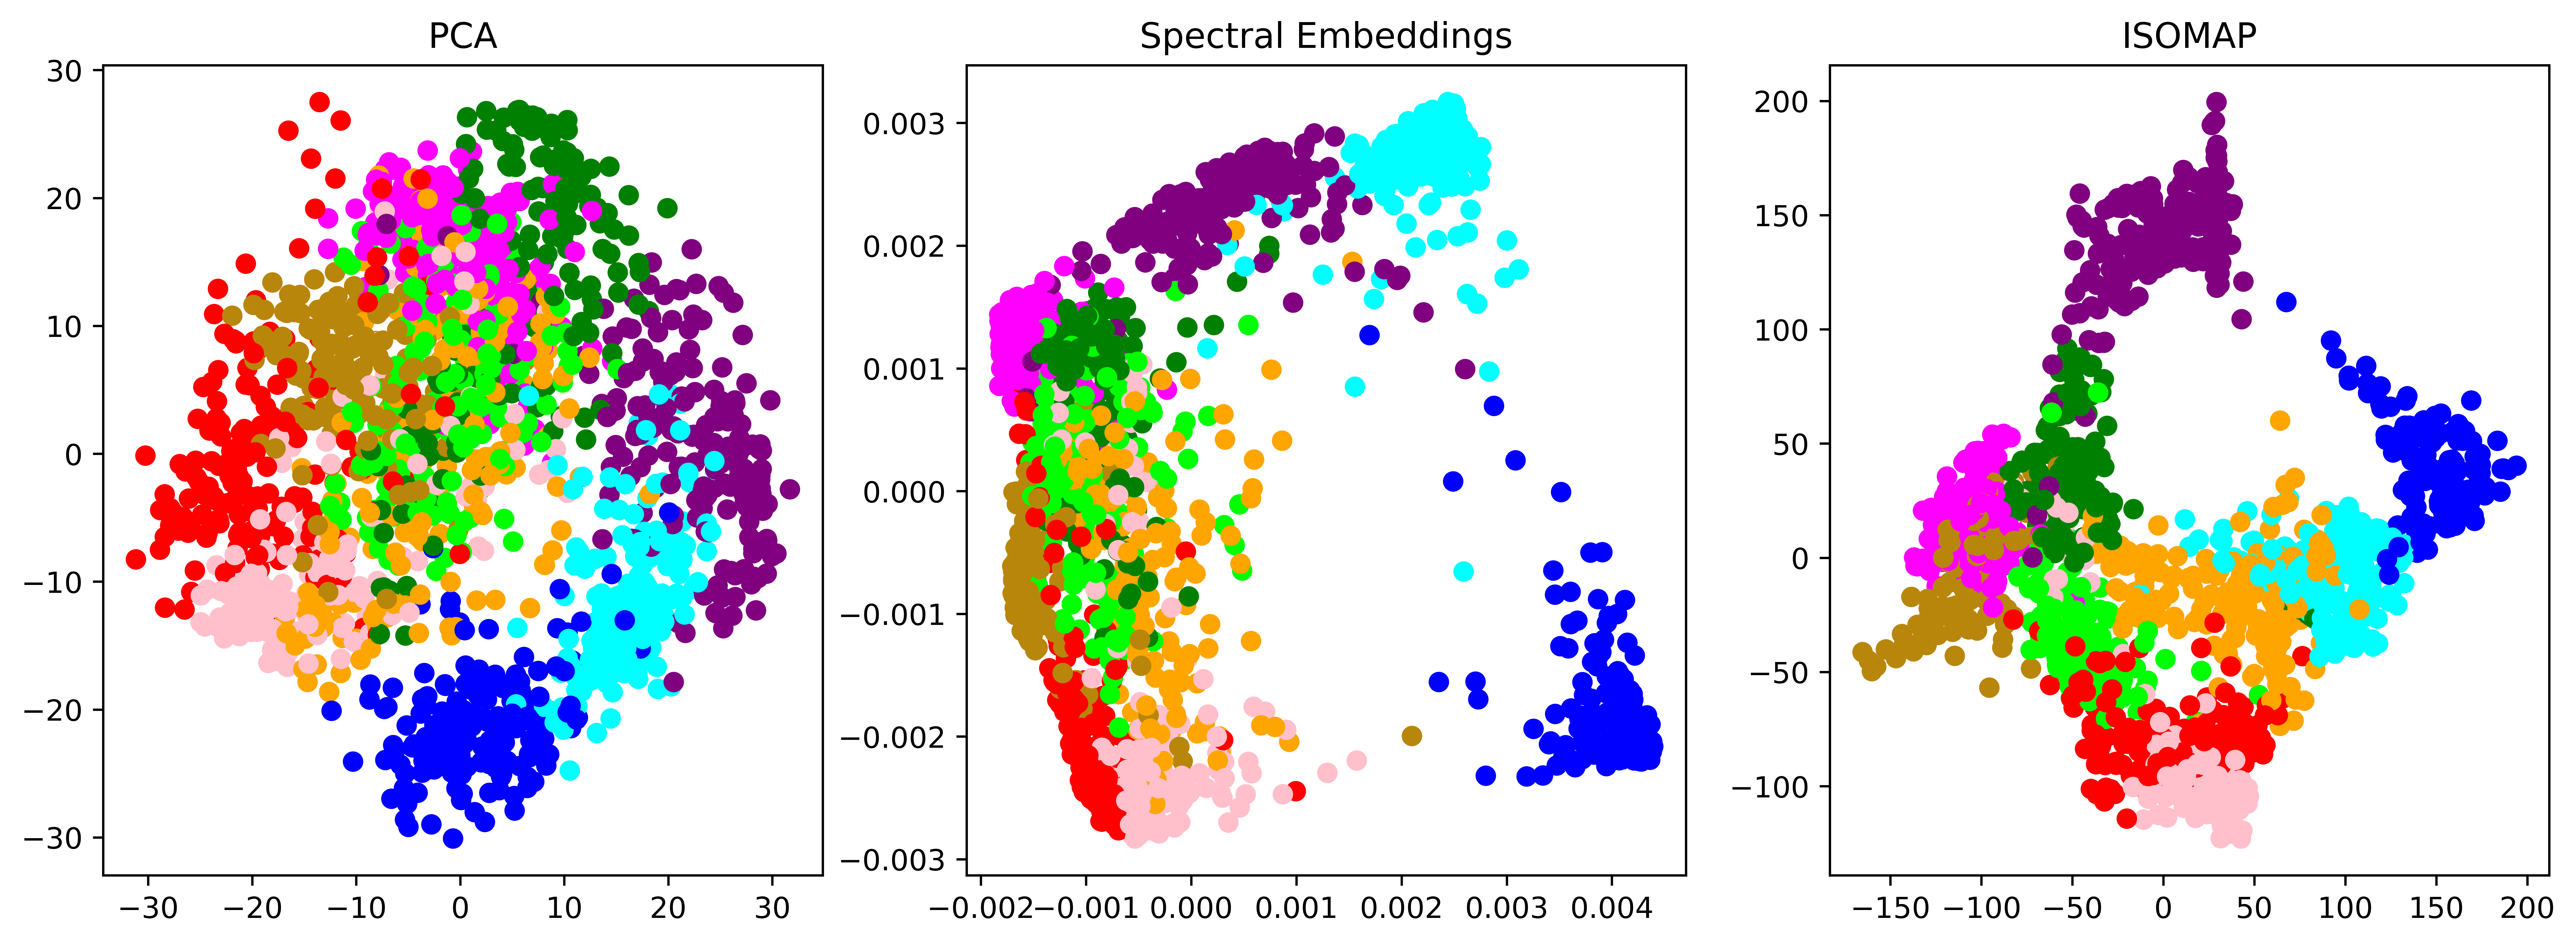
\includegraphics[width=0.99\linewidth]{images/decomposer/digits_decomposer_analysis.png}
                \caption{Визуализация набора данных Digits после снижения размерности до 2 с использованием PCA, Spectral Embeddings, ISOMAP.}
                \label{fig:digits:example}
            \end{figure}

            На рисунке \ref{fig:digits} представлены результаты экспериментов на наборе данных Digits. Следует отметить, что из-за ограничений существующей программной реализации методы Locally Linear Embeddings, MDS и UMAP не смогли корректно выполнить процедуру снижения размерности на этом наборе данных для последующей кластеризации и, таким образом, были исключены из анализа. Среди протестированных алгоритмов ярким лидером оказался ISOMAP, который уверенно превзошел остальные методы по всем основным метрикам кластеризации - AMI, ARI и NMI. Он продемонстрировал стабильное превосходство над базовой линией (результат кластеризации без снижения размерности) вплоть до размерности в 2 компоненты, что говорит о его способности сохранять глобальную геометрию данных даже в сильно сжатом пространстве. Метод PCA продемонстрировал устойчивую деградацию качества кластеризации при уменьшении числа компонент, особенно заметную ниже порога в 10 компонент. Это отражает его ограниченность в улавливании нелинейных зависимостей в данных. Spectral Embedding, напротив, показал результаты в целом ниже уровня базового \kmeans{}, что может объясняться тем, что он оптимизирует локальные отношения между точками, а не глобальную структуру. Тем не менее, на размерности, равной числу кластеров, наблюдался кратковременный всплеск метрик, что, вероятно, связано с тем, что алгоритм эффективно извлекает локальные кластеры, когда размерность достаточно для сохранения этих структур. Также была выявлена интересная зависимость по времени выполнения: ISOMAP, несмотря на свою сложность, в среднем демонстрировал сравнительно низкое время работы с редкими всплесками, что делает его не только точным, но и потенциально пригодным для практического применения при разумной конфигурации.

        \subsubsection{Результаты алгоритма на наборе данных Wine}
            Wine -- это стандартный и простой набор данных для многоклассовой классификации. Эти данные являются результатами химического анализа вин, выращенных в одном и том же регионе Италии тремя разными производителями. Существует тринадцать различных измерений, проведенных для различных компонентов, содержащихся в трех сортах вина.

            \begin{table}[H]
                \centering
                \caption{Характеристики набора данных Wine.}
                \begin{tabular}{ccc}
                    \toprule
                    Число классов &   Число объектов &   Размерность пространства \\
                    \midrule
                    3    &  178 &  13 \\
                    \bottomrule
                \end{tabular}
            \end{table}

            Набор данных Wine представляет собой матрицу с размерностью 178x13, где каждая строка соответствует отдельному образцу вина, а каждый столбец содержит значение конкретного химического измерения.

            \begin{figure}[H]\centering
                \subfigure[]{
                    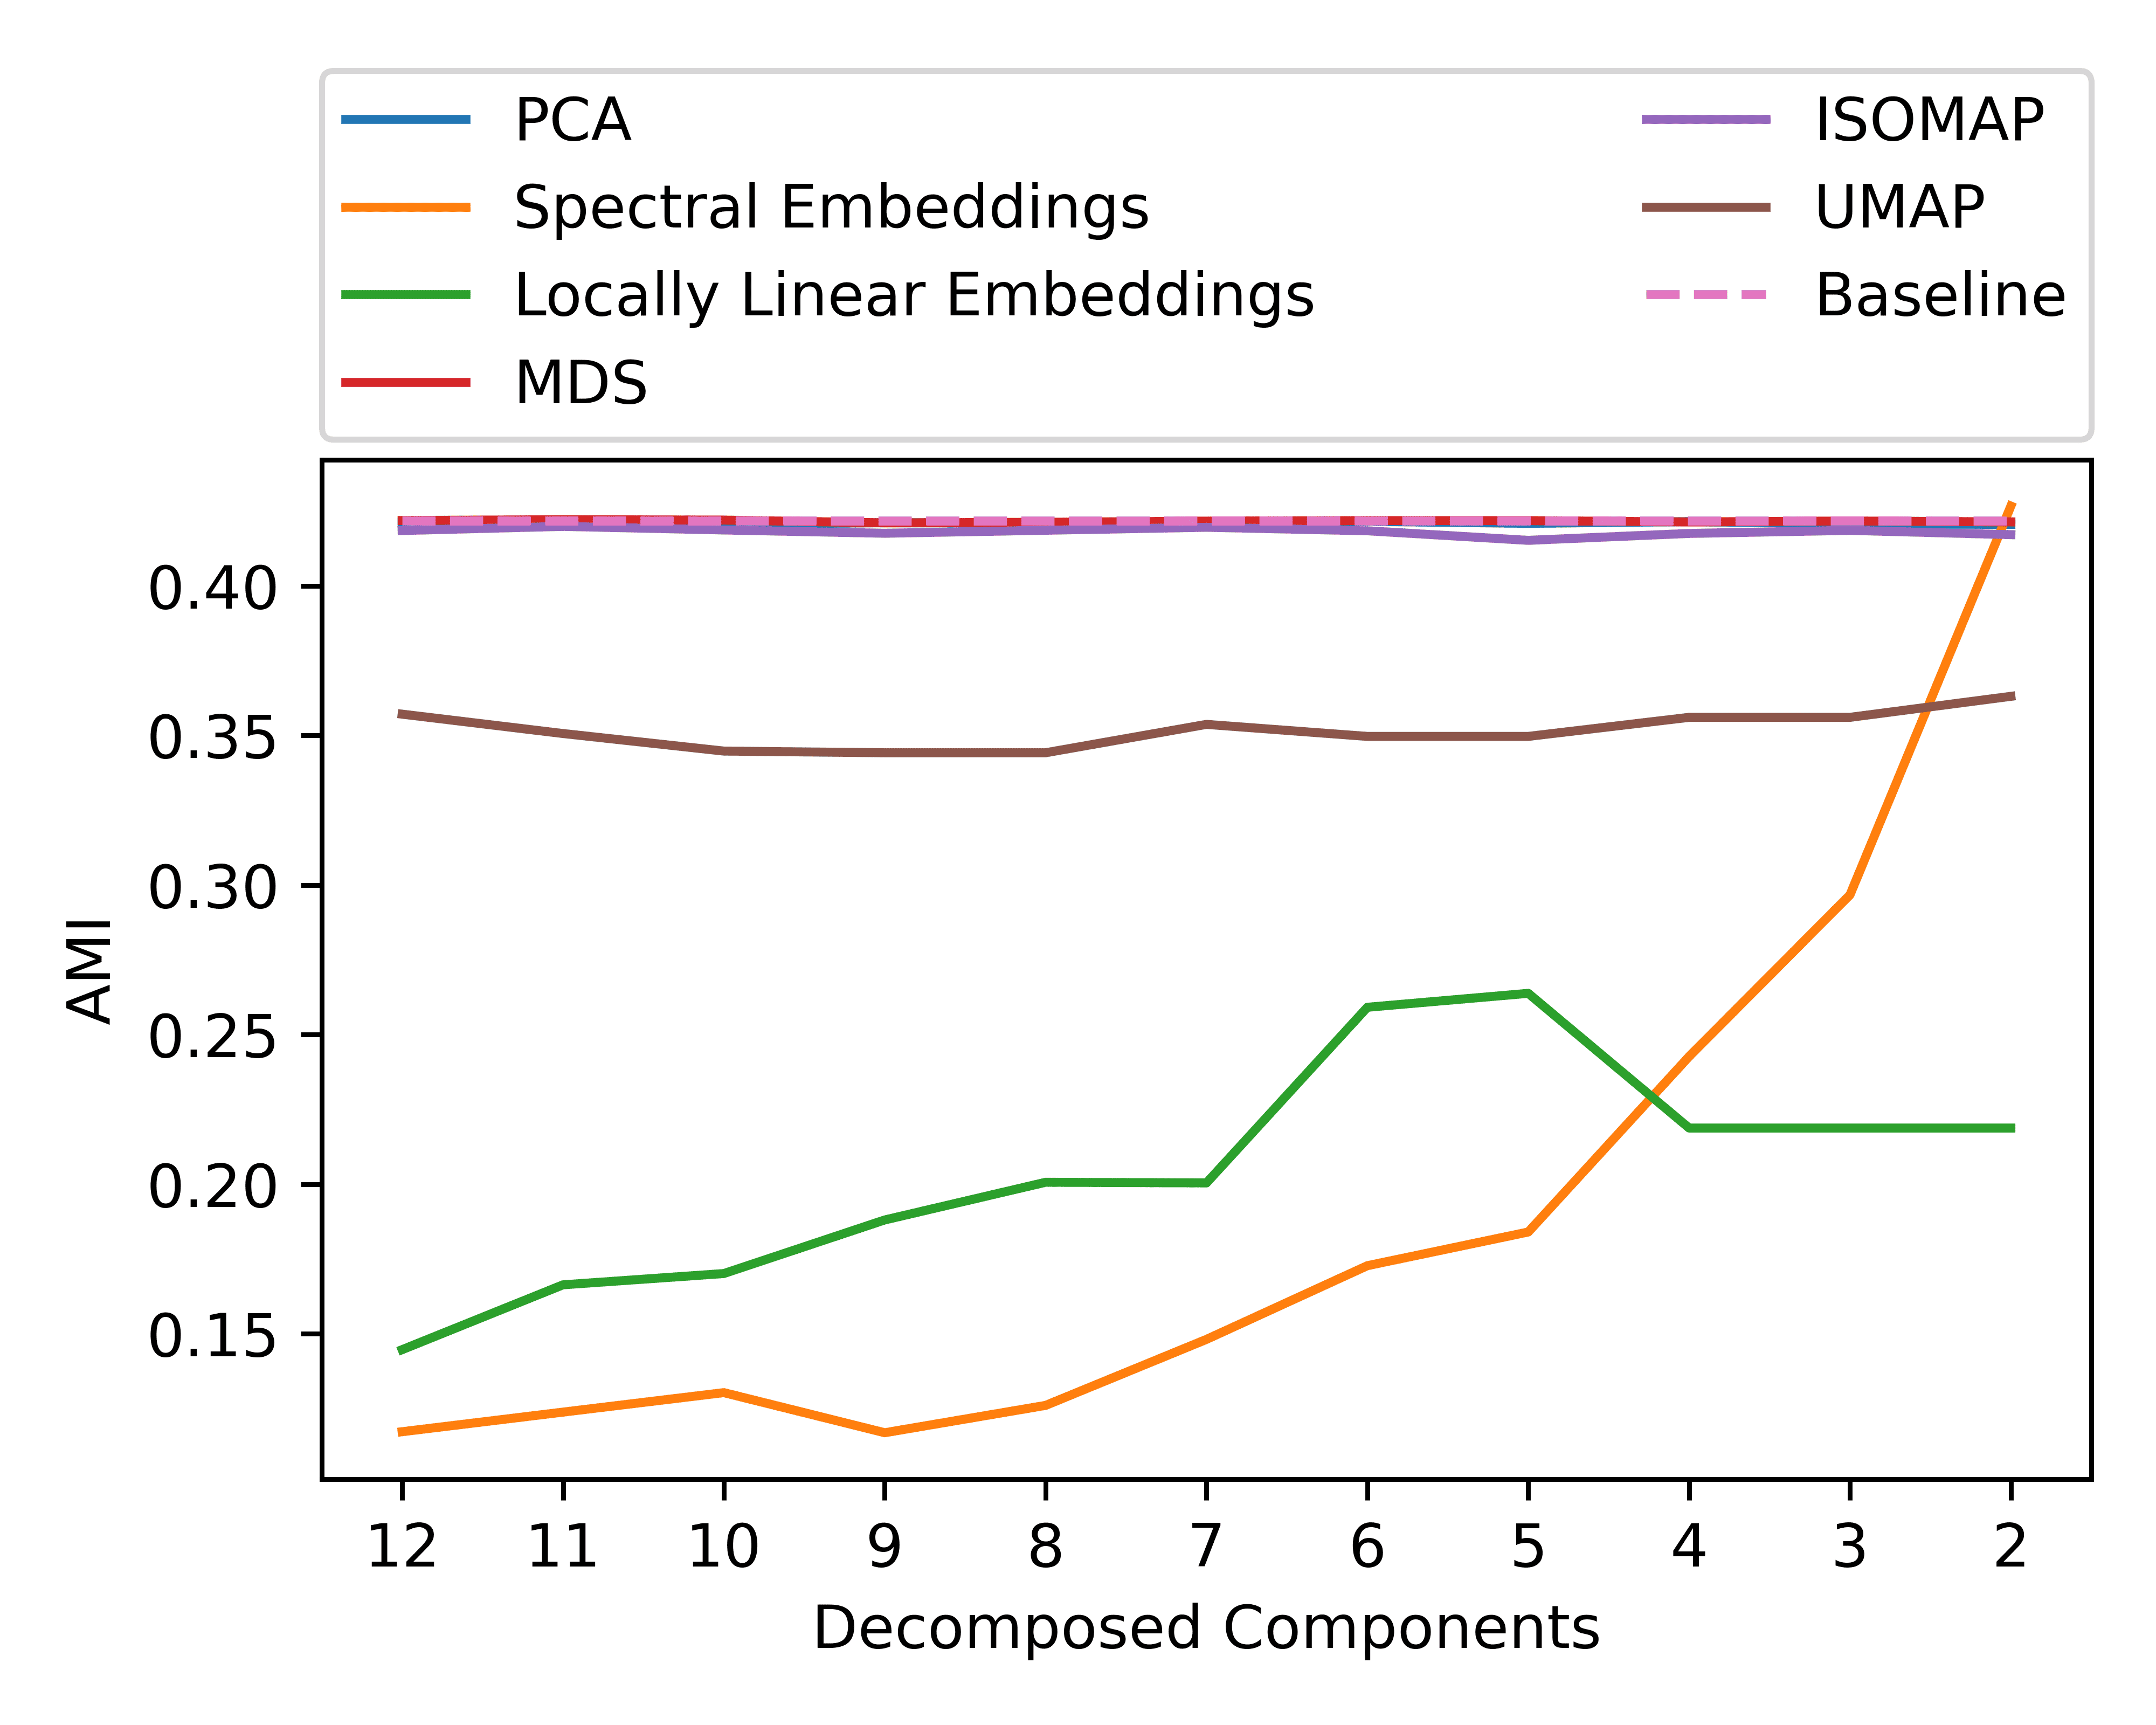
\includegraphics[width=0.48\linewidth]{images/charts_real/real_data_wine_ami.png}
                    \label{subfig:wine:ami}
                }
                \subfigure[]{
                    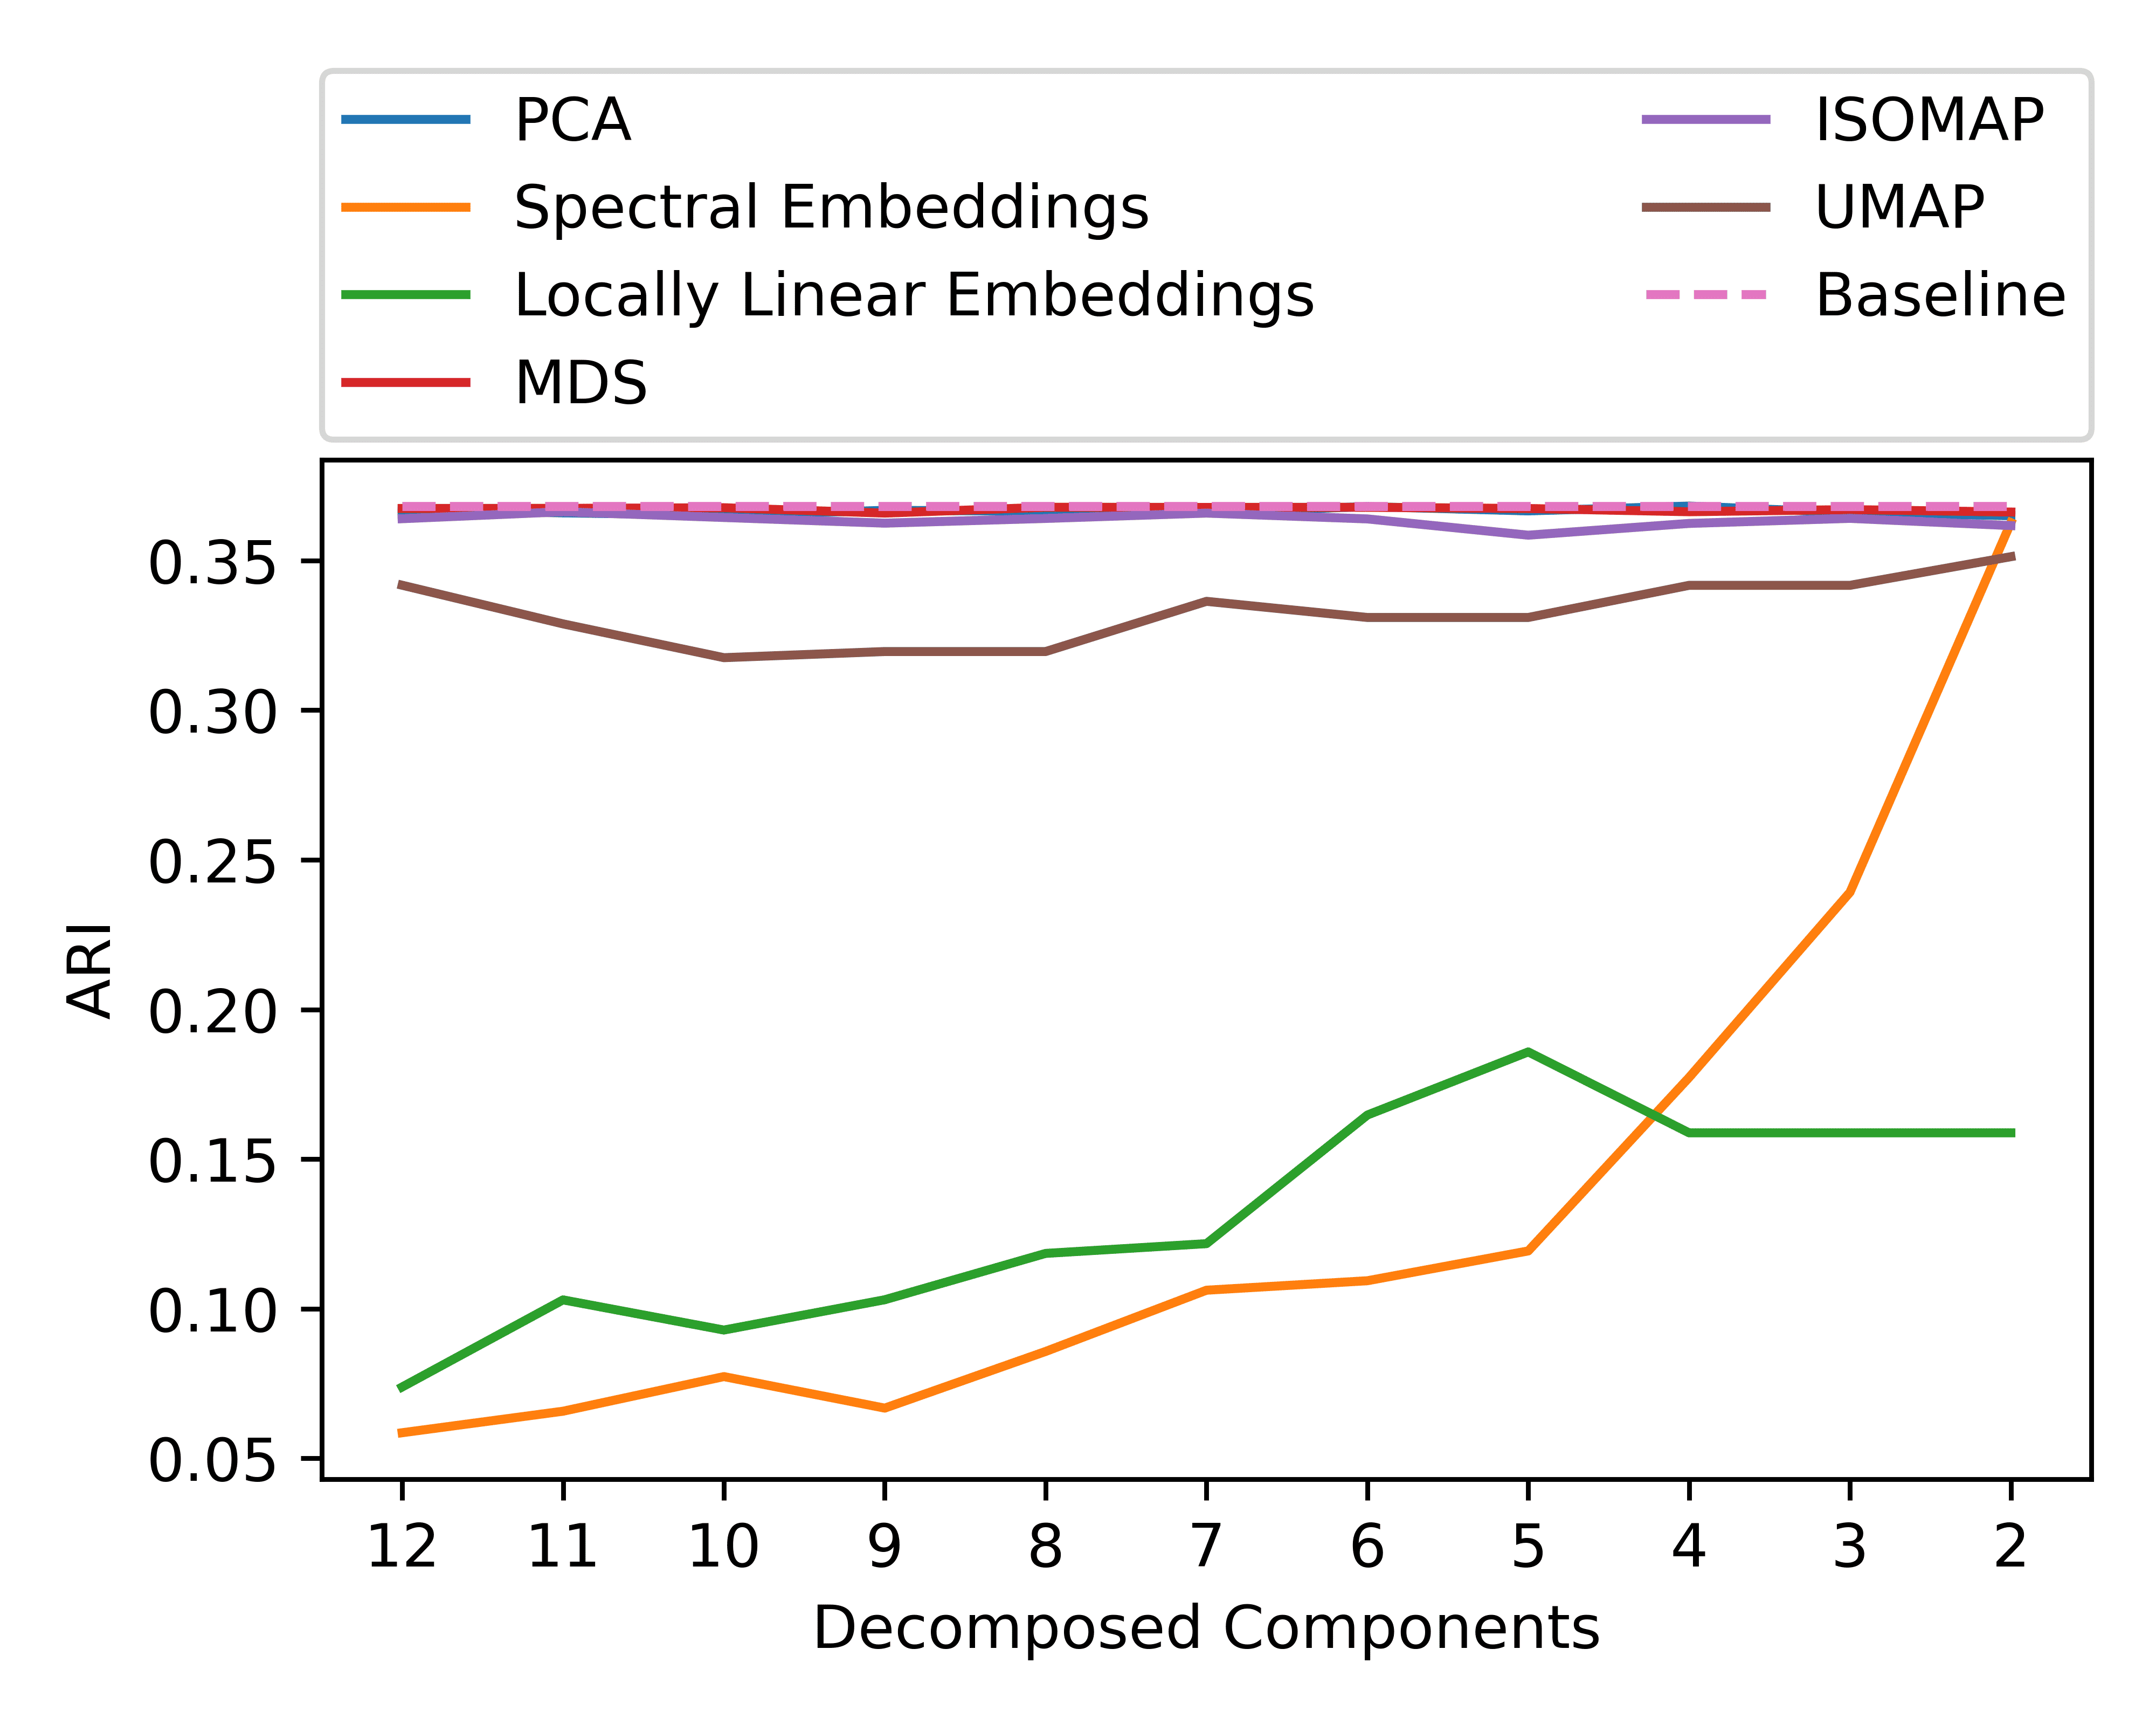
\includegraphics[width=0.48\linewidth]{images/charts_real/real_data_wine_ari.png}
                    \label{subfig:wine:ari}
                }
                \subfigure[]{
                    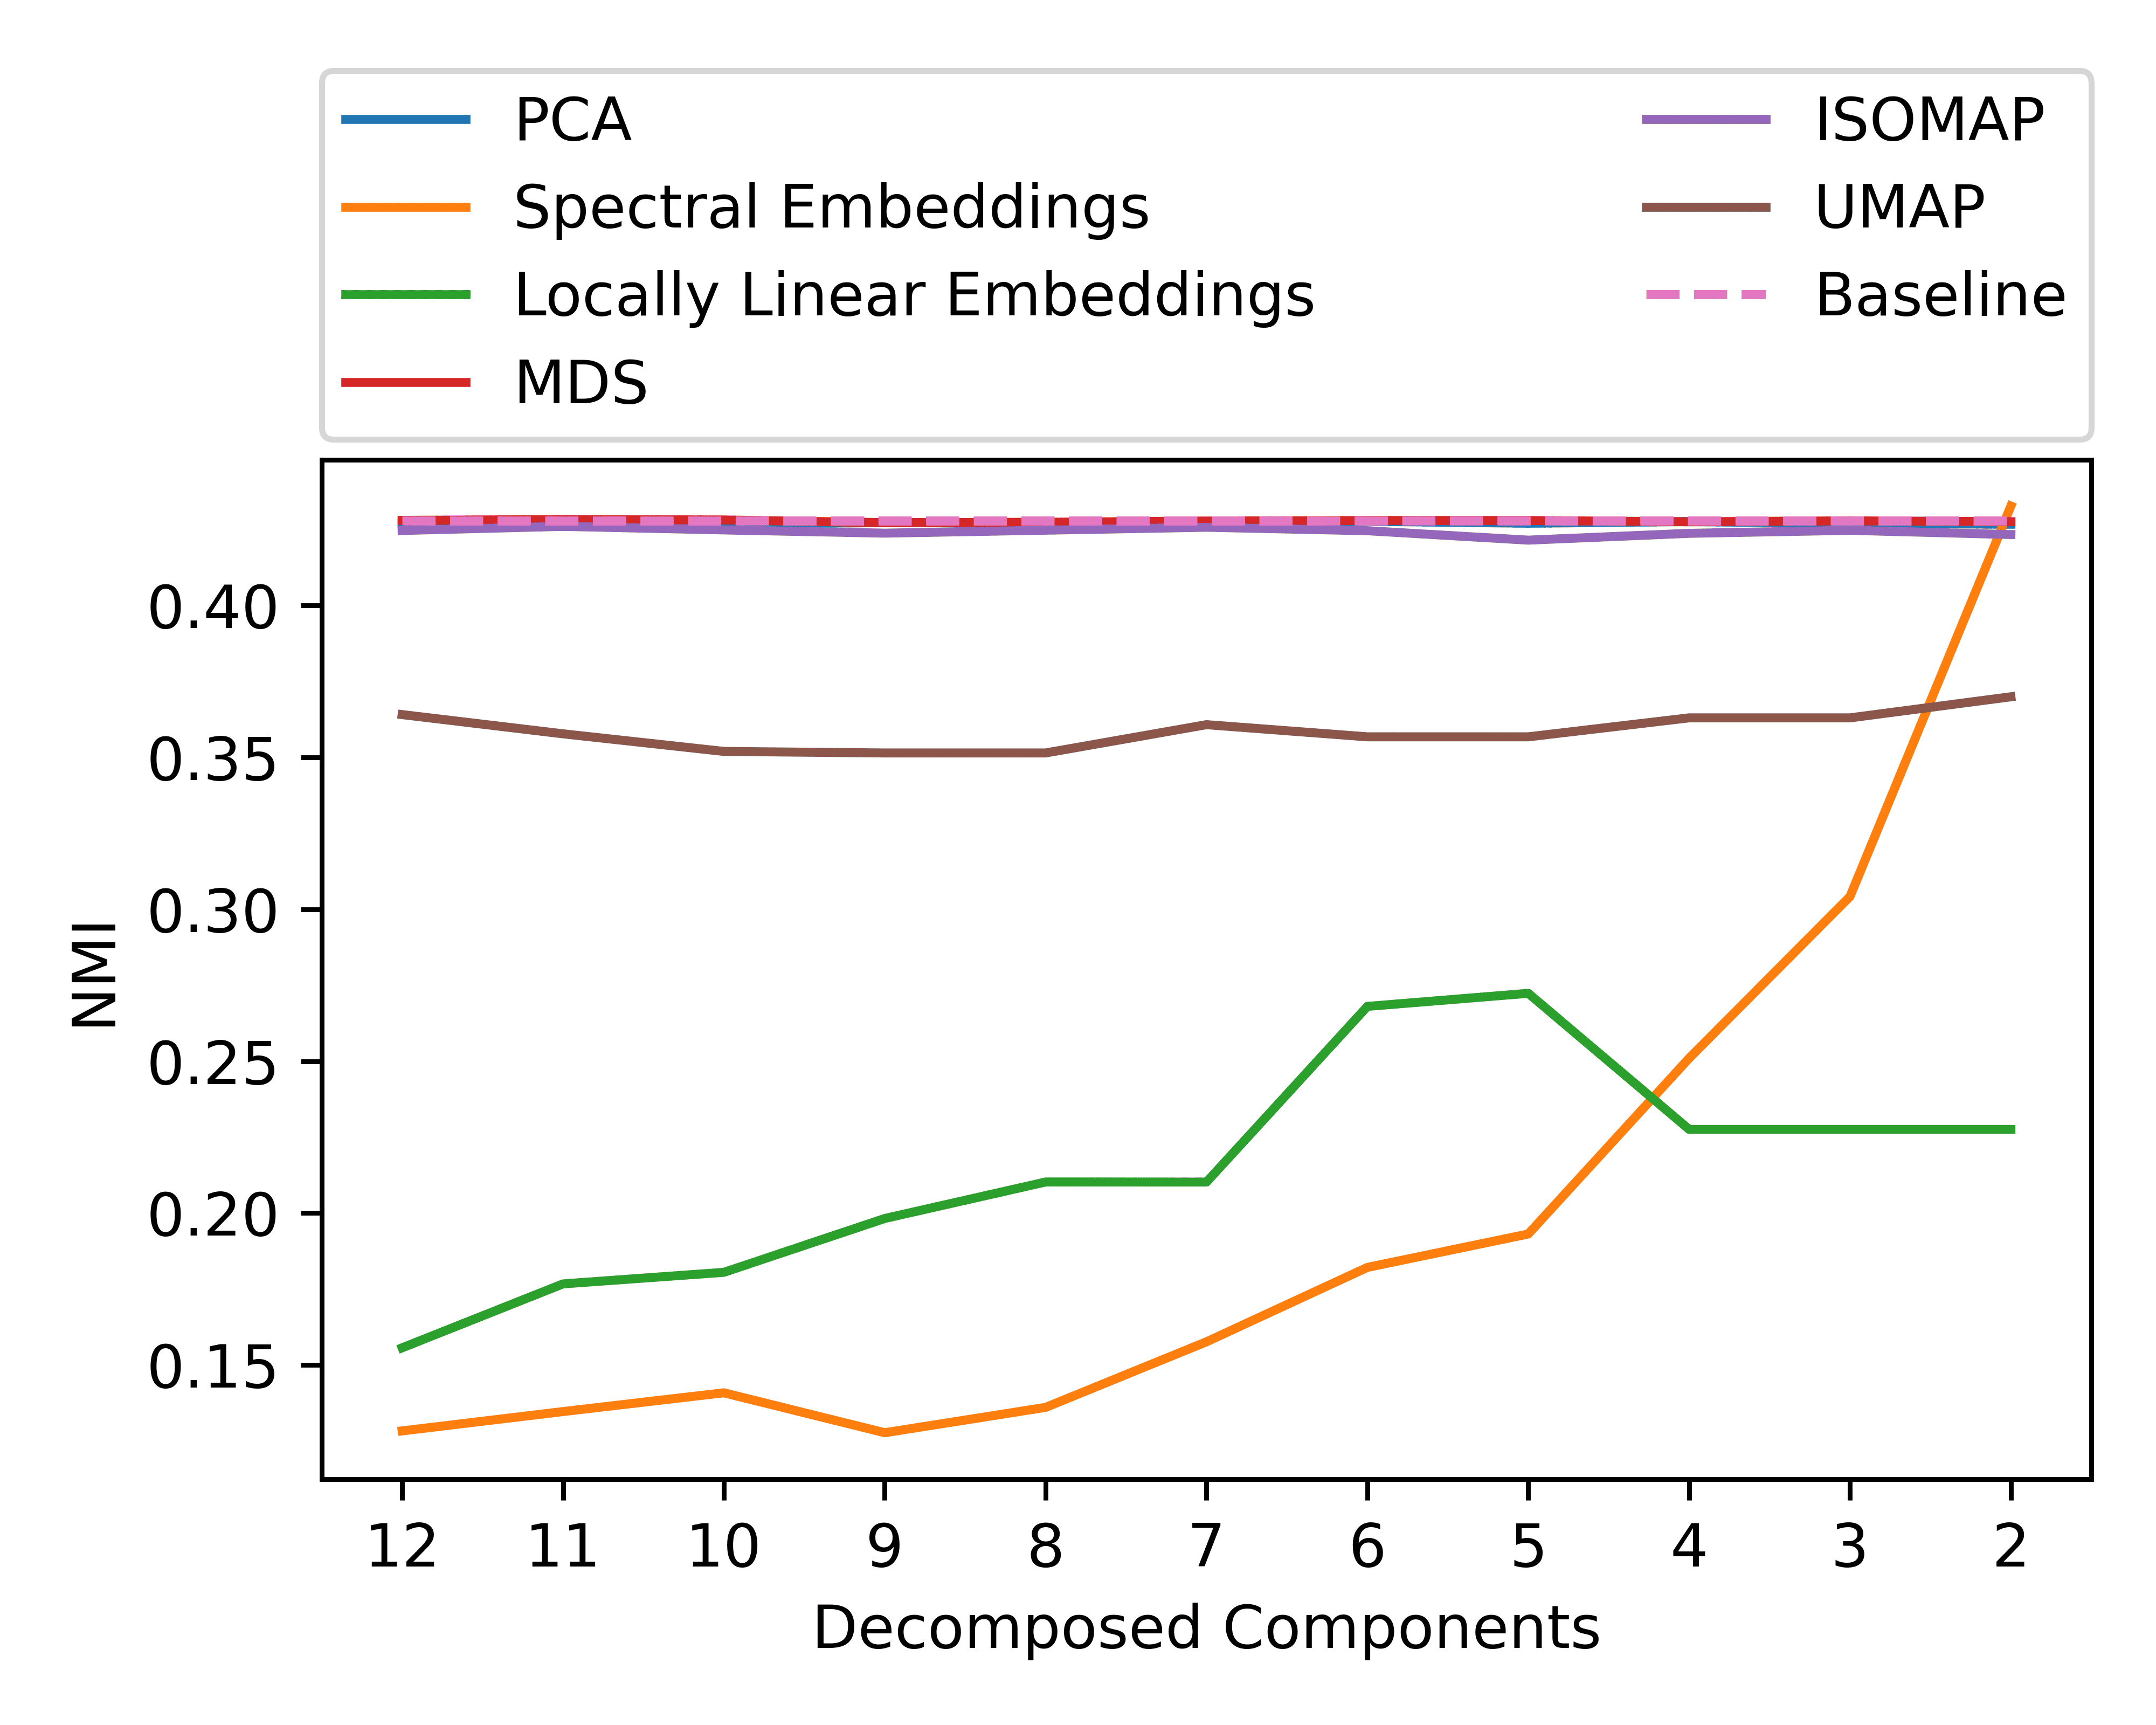
\includegraphics[width=0.48\linewidth]{images/charts_real/real_data_wine_nmi.png}
                    \label{subfig:wine:nmi}
                }
                \subfigure[]{
                    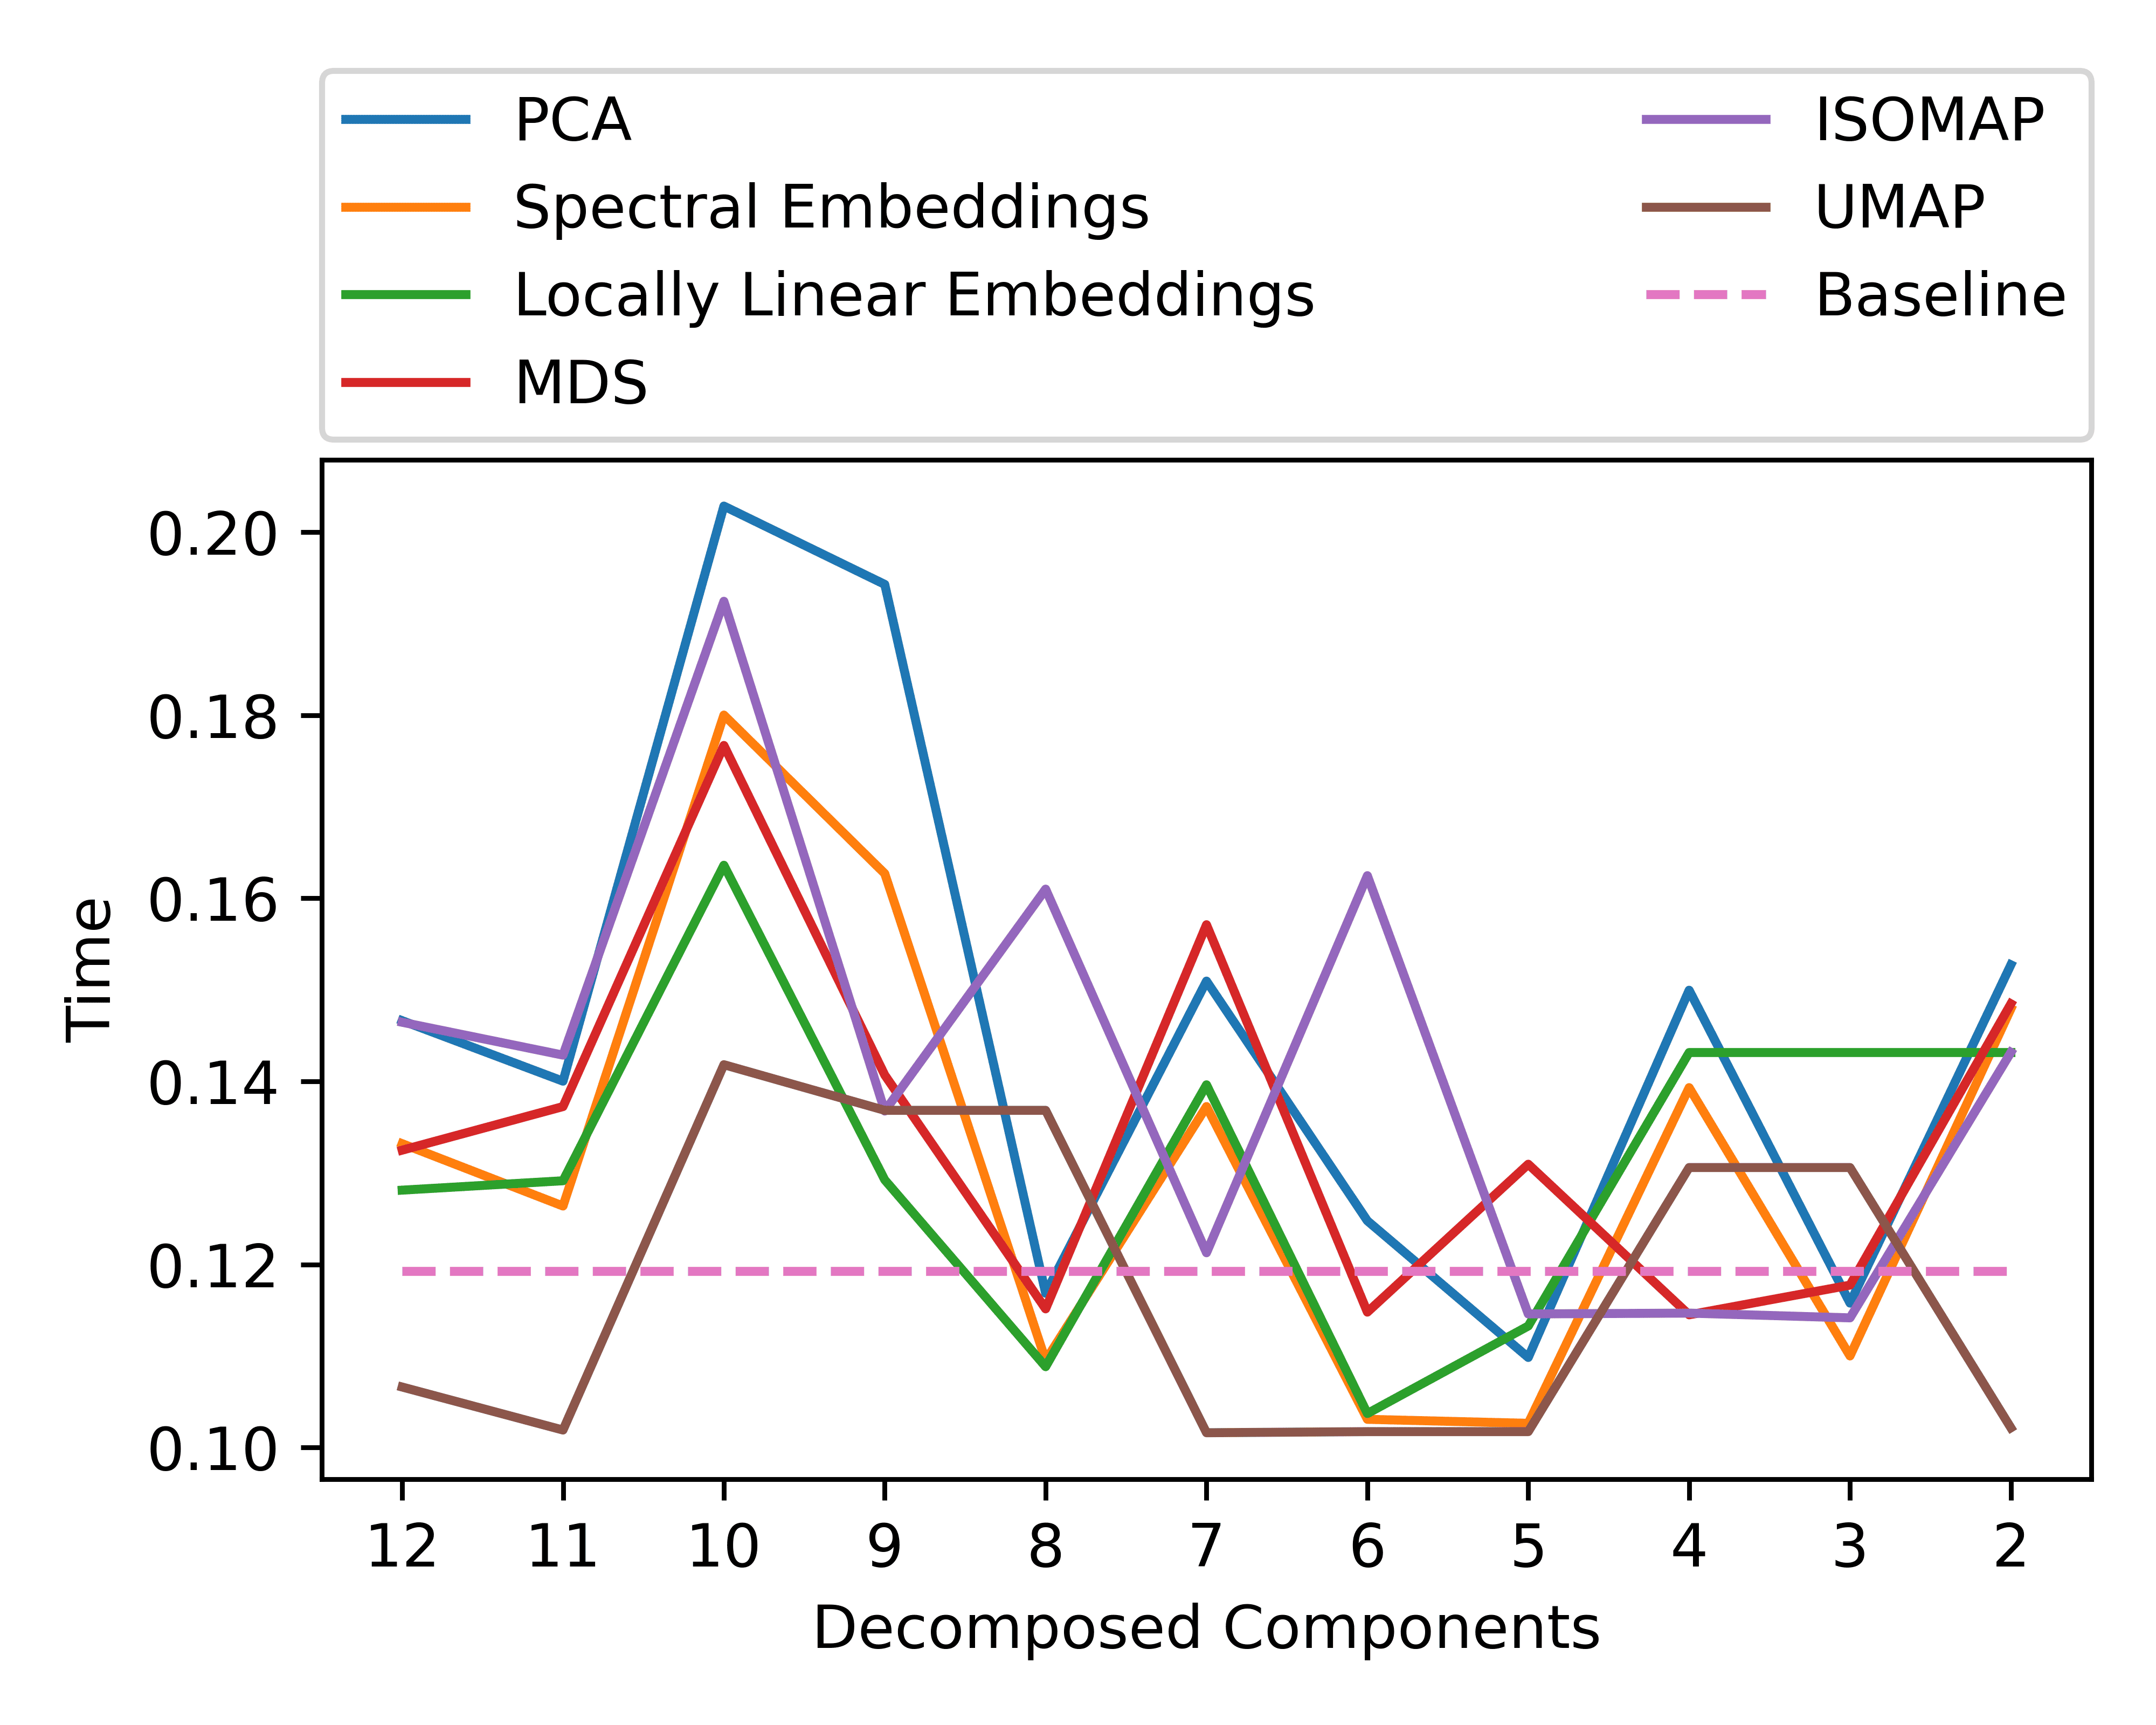
\includegraphics[width=0.48\linewidth]{images/charts_real/real_data_wine_time.png}
                    \label{subfig:wine:time}
                }
                \caption{Анализ влияния различных методов снижения размерности данных на кластеризацию набора данных Wine. Линия Baseline -- результат работы алгоритма \kmeans{} без предварительного снижения размерности. Результаты для
                    \subref{subfig:wine:ami} AMI;
                    \subref{subfig:wine:ari} ARI;
                    \subref{subfig:wine:nmi} NMI, а также на время работы алгоритма \subref{subfig:wine:time}.
                }
                \label{fig:wine}
            \end{figure}

            \begin{figure}[H]\centering
                \includegraphics[width=0.99\linewidth]{images/decomposer/wine_decomposer_analysis.png}
                \caption{Визуализация набора данных Wine после снижения размерности до 2 с использованием PCA, Spectral Embeddings, Locally Linear Embeddings, MDS, ISOMAP, UMAP.}
                \label{fig:wine:example}
            \end{figure}

            На рисунке \ref{fig:wine} представлены результаты экспериментов по кластеризации с предварительным снижением размерности на наборе данных Wine.
            Анализ показал, что методы PCA, ISOMAP и UMAP обеспечивают устойчивое поведение метрик, оставаясь на уровне или вблизи базовой линии на всем диапазоне компонент. Однако, несмотря на эту стабильность, они не продемонстрировали прироста качества кластеризации при уменьшении размерности. В то же время, методы Locally Linear Embeddings (LLE) и Spectral Embeddings показали заметное улучшение показателей AMI, ARI и NMI при переходе к малым числам компонент. Значительный прирост качества заметен у метода Spectral Embeddings, достигающий пика на 2-х компонентах, и опережающий качество исходной кластеризации. Это указывает на его способность извлекать более информативную структуру данных в условиях значительного снижения размерности.
